\documentclass{dissertation}

\usepackage[version=4]{mhchem}
\usepackage{siunitx}
\usepackage{pdflscape}
\usepackage{enumitem}
\usepackage[final]{pdfpages}
\usepackage{booktabs}
\usepackage{longtable}
\usepackage{multirow}
\usepackage{setspace}
\usepackage{nameref}

\theoremstyle{definition}
\newtheorem*{objective}{Objective}
 
\theoremstyle{remark}
\newtheorem*{constraint}{Constraints}

\newcommand{\ra}[1]{\renewcommand{\arraystretch}{#1}}

\newcommand{\compresslist}{
	\setlength{\itemsep}{1pt}
	\setlength{\parskip}{0pt}
	\setlength{\parsep}{0pt}
	}
%\onehalfspacing

\begin{document}

%% Specify the title and author of the thesis. This information will be used on the title page (in title/title.tex) and in the metadata of the final PDF.

% Thesis Title
% Format: \title[Optional Subtitle]{Title}
\title[Development of the Corrosion Modelling Application Yellowjacket]{Calculating Thermochemical Equilibrium for Multiphysics Simulations of Nuclear Materials} 
%\subtitle{Development of Corrosion Modelling Application Yellowjacket}

% Author Name
% Format: \author{Firstname}{Lastname}
\author{Parikshit}{Bajpai}

% Degree and Program
% Format: \DegreeProgram{Degree}{Program}
\DegreeProgram{Doctor of Philosophy}{Modelling and Computational Science}

% Thesis month and year
% Format: \DefenseDate{Month}{Year}
\DefenseDate{30}{October}{2022}

%% Use Roman numerals for the front matter.
\frontmatter

% Title page
\begin{titlepage}

%\begin{center}
%
%
%%% Extra whitespace at the top.
%\vspace*{2\bigskipamount}
%
%%% Print the title.
%{\makeatletter
%\CoverFont{b}{18}{20pt}\LARGE\@title
%\makeatother}
%
%%% Print the optional subtitle.
%{\makeatletter
%\ifx\@subtitle\undefined\else
%    \bigskip
%    \titlefont\titleshape\Large\@subtitle
%\fi
%\makeatother}
%
%\end{center}
%
%\cleardoublepage
\thispagestyle{empty}

\begin{center}

%% The following lines repeat the previous page exactly.

\vspace*{2\bigskipamount}

%% Print the title.
{\makeatletter
\CoverFont{b}{18}{20pt}\LARGE\@title
\makeatother}

%% Print the optional subtitle.
{\makeatletter
\ifx\@subtitle\undefined\else
    \bigskip
    \CoverFont{m}{12}{14pt}\Large\@subtitle
\fi
\makeatother}

%% Uncomment the following lines to insert a vertically centered picture into
%% the title page.
%\vfill
%\includegraphics{title}

%% Apart from the names and dates, the following text is dictated by the
%% promotieregelement.

\bigskip
\bigskip
\bigskip
\bigskip
\bigskip
\bigskip

by

\bigskip
\bigskip

%% Print the full name of the author.
\makeatletter
{\bf \@firstname\ {\@lastname}}
\makeatother

\bigskip
\bigskip
\bigskip
\bigskip

A thesis submitted to the\\
School of Graduate and Postdoctoral Studies\\
in partial fulfilment of the requirements for the degree of 

\bigskip
\bigskip
\bigskip
\bigskip

{\bf{\degree}}

% \medskip

in

%  \medskip

{\bf{\program}}

\bigskip
\bigskip
\bigskip
\bigskip

School of Graduate and Postdoctoral Studies 

\medskip

University of Ontario Institute of Technology (Ontario Tech University)

\medskip

Oshawa, Ontario, Canada

\medskip
\degreemonth{} \degreeyear

\vfill


\bigskip
\textcopyright{} \makeatletter \@firstname\ {\@lastname}\makeatother, \degreeyear


%\date{\today}

%% Extra whitespace at the bottom.
\vspace*{2\bigskipamount}

\end{center}

\end{titlepage}


% Thesis exam information

\cleardoublepage
\thispagestyle{plain}

%% The following line is dictated by the promotieregelement.
\begin{center}
\textbf{THESIS EXAMINATION INFORMATION}

\bigskip

Submitted by:  \makeatletter\textbf{\@firstname\ {\@lastname}}\makeatother

\bigskip
\bigskip

\textbf{\degree} in \textbf{\program}

\end{center}


\bigskip
\bigskip

\noindent \fbox{
    \parbox{\textwidth}{Thesis title: \makeatletter\textbf{\@title}\makeatother}
}

\bigskip

An oral defense of this thesis took place on DATE OF DEFENCE in front of the following examination committee:

\medskip

\noindent\textbf{Examining Committee:}

\bigskip

\begingroup
\renewcommand{\arraystretch}{2}
\begin{tabular}{lcl}
    Chair of Examining Committee &\phantom{Alphabet}& NAME \\
    Research Supervisor && NAME\\
    Research Co-supervisor && NAME \\
    Examining Committee Member && NAME \\
    Examining Committee Member && NAME \\
    Thesis Examiner && NAME, Affiliation (For Masters only)\\
    University Examiner && NAME \\
    External Examiner && NAME, Affiliation (For PhD only)\\
\end{tabular}
\endgroup

\medskip

\noindent The above committee determined that the thesis is acceptable in form and content and that a satisfactory knowledge of the field covered by the thesis was demonstrated by the candidate during and oral examination. A signed copy of the Certificate of Approval is available from the School of Graduate and Postdoctoral Studies.





\chapter*{Abstract}
\addcontentsline{toc}{chapter}{Abstract}
\setheader{Abstract}

Nuclear fuels and structural materials are highly complex systems that are remarkably challenging to understand and model. Material behaviours are influenced by multiple physical phenomena such as mechanics, chemistry, heat and mass transport, etc. Moreover, lower scale phenomena inform and drive the phenomena at larger scales. The strong interactions between multiple physics at different length and time scales creates a need for multi-scale, multi-physics modelling tools. In nuclear fuels and structural materials, the problem gets compounded by the fact that, in addition to an extreme environment, the composition of the system changes with time. For such complex systems, computational thermodynamics plays a valuable role in predicting many phenomena and is, often necessary for understanding and informing others. For this reason, there has been an increasing interest in incorporating equilibrium thermodynamics calculation in multi-physics frameworks such as Multiphysics Object Oriented Simulation Environment (MOOSE). To simulate corrosion in molten salt reactors, a new MOOSE-based tool named {\YJ} has been developed and this work contributes to it.

The objective of this work is to develop a new equilibrium thermodynamic solver to provide thermodynamic material properties and boundary conditions for {\YJ} and other MOOSE-based codes. While several thermodynamics codes already exist, the new software, called {\GEM}, adds native equilibrium thermodynamic capability to MOOSE and aims to address several concerns such as computational performance, limitations on system size and models, and Software Quality Assurance (SQA).

{\GEM} exploits the fundamental laws of thermodynamics to solve a non-linear, non-convex optimisation problem. Several thermodynamic models, including the Modified Quasichemical Model in Quadruplet Approximation (MQMQA) were implemented, and state-of-the-art numerical solvers in Portable, Extensible Toolkit for Scientific Computation (PETSc) were used to efficiently solve the optimisation problem. In doing so, the work contributes to the understanding of MQMQA which until recently wasn't well comprehended. Ensuring that the solver gives a true equilibrium solution also requires solving a global optimisation problem without severely compromising performance and reliability. Several global optimisation methods were compared through numerical experiments to objectively select the best approach for implementation. The C++ code follows MOOSE coding standards and SQA procedures and enables direct coupling of thermodynamic equilibrium calculations in multiphysics simulations performed using MOOSE. 


%======================= Version 2 =======================
%Nuclear fuels and structural materials are highly complex systems that have traditionally been challenging to understand and model. Material behaviour is influenced by many different phenomena such as mechanics (dislocations, cracking, etc.), chemistry (oxidation, reactive transport, corrosion, etc.), heat and mass transport, amongst many others. Moreover, lower length scale phenomena inform and drive the phenomena at larger scales. The strong interactions between multiple physics at different length and time scales creates a need for multi-scale, multiphysics modelling tools which aim to use lower scale information to inform the models at larger scales with the goal of improving the predictive performance of models and simulations. In nuclear fuels, the problem gets compounded by the fact that, in addition to extreme environment, nuclear fission leads to formation of numerous fission products and the composition of the system changes with time. Transmutations and other phenomena lead to similar evolution of composition in structural materials as well, albeit to a lesser extent. For such complex systems, computational thermodynamics plays a key role in predicting many phenomena and is, at minimum, necessary for understanding and informing others. For this reason, there has been an increasing interest in incorporating equilibrium thermodynamics calculation in multiphysics frameworks such as Multiphysics Object Oriented Simulation Environment (MOOSE).
%
%A phenomena of particular interest in advanced reactors that employ high-temperature fluids such as molten salts is that of corrosion of fluid facing structural materials. Since corrosion is an electrochemical process occurring at the microstructural level and is driven by the thermodynamics and redox kinetics of the system, a new MOOSE-based tool, namely {\YJ}, has been developed to predict quantities such as the rate of material loss, corrosion product production, and precipitate production in liquid. The primary objective of this work is to develop a new equilibrium thermodynamic solver to provide thermodynamic material properties and boundary conditions for {\YJ} and other MOOSE-based simulation codes. While several thermodynamics codes already exist, the new software, called {\GEM}, aims to bring native equilibrium thermodynamic capability to the MOOSE framework and at the same time aims to address several concerns related to the current codes, specifically, computational performance, limitations on system size and models, and software quality assurance.


%======================= Version 1 =======================
%Many emerging nuclear technologies, such as the Molten Salt Reactor (MSR), use high temperature fluids such as molten fluoride/chloride salts, which lead to corrosion of the metal containment leading to problematic behaviours during reactor operations. Corrosion is an electrochemical process composed of oxidation and reduction reactions, which are driven by the thermodynamics and kinetics of the reactions. While thermodynamics determines whether or not a material can corrode, kinetics influences how quickly the material will corrode. This corrosion behaviour is also significantly affected by the material microstructure and predicting corrosion therefore requires a multiphysics approach that can couple quantitative electrochemistry models of corrosion and chemical reactions with thermochemical equilibrium computations. The Multiphysics Object Oriented Simulation Environment (MOOSE) developed by the Idaho National Laboratory provides a framework for multiphysics simulations but lacks the tools for predicting corrosion at the microstructure scale. Under Nuclear Energy Advanced Modelling and Simulation Program, a new MOOSE-based tool, YellowJacket, has been developed to perform such simulations and to predict quantities such as the rate of material loss, corrosion product production, and precipitate production in liquid.
%
%As part of YellowJacket, a new thermochemical equilibrium solver, YellowJacket-GEM, was developed to quantitatively provide quantities of interest, for example chemical potential of stable species, by using the principles of thermodynamics. YellowJacket-GEM replaces many empirically based models for material properties and boundary conditions with a fundamentally sound approach that is founded on fundamental principles of thermodynamics while also reducing the computational cost associated with such coupling. The Gibbs energy minimiser uses state-of-the-art mathematical solvers and  global optimisation algorithms to reduce computational cost and improve accuracy of thermochemical equilibrium and is fully compatible with the MOOSE programming architecture in a cohesive manner using the same programming language and software libraries while satisfying the same software quality metrics and improving the thermodynamic capability. The coupling of YellowJacket-GEM with MOOSE phase field module to model corrosion in MSRs has also been performed and demonstrated.

\bigskip
\bigskip
\bigskip
\bigskip

\noindent
\textbf{Keywords:} Computational Thermodynamics; Gibbs Energy Minimisation; Global Optimisation; {\YJ} Gibbs Energy Minimiser; Mutiphysics Object Oriented Simulation Environment (MOOSE)


\chapter*{Author's Declaration}
\addcontentsline{toc}{chapter}{Author's Declaration}
\setheader{Author's Declaration}


I hereby declare that this thesis consists of original work of which I have authored. This is a true copy of the thesis, including any required final revisions, as accepted by my examiners.


I authorize the University of Ontario Institute of Technology (Ontario Tech University) to lend this thesis to other institutions or individuals for the purpose of scholarly research. I further authorize University of Ontario Institute of Technology (Ontario Tech University) to reproduce this thesis by photocopying or by other means, in total or in part, at the request of other institutions or individuals for the purpose of scholarly research. I understand that my thesis will be made electronically available to the public.

\bigskip
\bigskip

\makeatletter\textbf{\@firstname\ {\@lastname}}\makeatother


\chapter*{Statement of Contributions}
\addcontentsline{toc}{chapter}{Statement of Contributions}
\setheader{Statement of Contributions}
Some of the work presented in this thesis was completed as part of coauthored works and the main body of this thesis reflects the contributions made as the primary author. Where the work as a secondary author has been presented, it has been significantly abridged to emphasise only the significant contribution of the author of this thesis and the same has been acknowledged in the text. 

In section~\ref{sec:ChemPotExp}, the following two articles have been used with permission from the publisher:
\begin{enumerate}{\small \compresslist
    \item {P.\ Bajpai}, {M.\ Poschmann}, {M.H.A.\ Piro}, \textit{Derivations of useful partial molar excess Gibbs energy of mixing expressions of common thermodynamic models}, {Journal of Phase Equilibria and Diffusion, 42 (2021) 333-347}. 
The author of this thesis was solely responsible for performing the analysis and mathematical derivations and was co-responsible for the verification along with M.\ Poschmann. The author also wrote the majority of the manuscript. 
    
    \item {M.\ Poschmann}, {P.\ Bajpai}, {B.W.N.\ Fitzpatrick}, {M.H.A.\ Piro}, \textit{Recent developments for molten salt systems in Thermochimica}, {Calphad, 75 (2021) 102341}. 
Thesis author's main contribution was the analysis of the MQMQA and derivation of expressions presented in section 2 of the article. Both these activities were performed in conjunction with the primary author of the paper. As such, only section 2 has been presented here and the other sections of the article which do not represent the author's contribution have been omitted.
   }
\end{enumerate}


In section~\ref{sec:algo_choice}, the article: {P.\ Bajpai}, {M.H.A.\ Piro}, \textit{Corrigendum to `The thermochemistry library Thermochimica'}, {Computational Materials Science, 198 (2021) 110659}, has been used with permission from the publisher. The author of this thesis carried out all the analysis and wrote the manuscript. M.H.A. Piro conceptualised and revised the manuscript.


The work described in chapter~\ref{chap:implementation} was performed, in part, during a virtual internship at the Idaho National Laboratory (Idaho Falls, Idaho, United States). The work was performed under the supervision of Dr. Daniel Schwen and the thesis author was responsible for design and implementation of the software. Dr. Daniel Schwen reviewed the code and suggested minor code patches.

In section~\ref{sec:interpret_res}, the article {M.H.A.\ Piro}, {M.\ Poschmann}, {P.\ Bajpai}, \textit{On the interpretation of chemical potentials computed from equilibrium thermodynamic codes: Applications to molten salts}, {Journal of Nuclear Materials, 526 (2019) 151756} was used with permission from the publisher. Thesis author contributed to the discussion which evolved into the letter and co-authored the example section of the manuscript.

In section~\ref{sec:gem_pf}, results from a coupled simulation are presented. This work was performed in collaboration with C. Bhave of University of Florida. The author of this thesis was responsible for the development of the thermodynamic equilibrium solver and for all the thermodynamic calculations performed as part of the simulation. C. Bhave performed the phase-field part of the simulation.

\chapter*{Acknowledgements}
\addcontentsline{toc}{chapter}{Acknowledgements}
\label{acknowledgements}

I am deeply grateful to my supervisor Prof. Markus Piro for not only giving me the opportunity to work this research but also for his constant guidance and encouragement. His contribution to this work and to my development as a researcher has been invaluable and his advice and enthusiasm has made this work extremely rewarding and delightful. I can't appreciate enough the support of Dr. Daniel Schwen who mentored me as an intern at the Idaho National Laboratory and from whom I have learnt innumerable things about MOOSE but more importantly on how to design and write good code.

This work has benefited from the numerous discussions with our collaborators, Chaitanya Bhave and Prof. Michael Tonks from the University of Florida. These discussions provided a great insight into the objectives and were always useful in deciding the direction we want to pursue with the development of the code and its coupling with the phase field code developed by Chaitanya. Along the same lines, I must also thank Dr. Ben Spencer, Prof. Ted Besmann, Dr. Jake McMurray and Dr. David Andersson, as the leaders of the NEAMS Chemistry and Corrosion technical area facilitated and guided this work. % I would like to thank Dr. Rich Martineau who initiated this work and Dr. David Andrs who supported the initial development of the code.

I wish to thank Prof. Lennaert van Veen and Prof. Hendrick de Haan who have provided constant help as members of the supervisory committee and also to the members of the examining committee Prof. Kirk Atkinson and Prof. Greg Lewis for taking time out of their very busy schedules to review this work. In particular, I would like to thank Prof. Maria Emelianenko (George Mason University) for very kindly agreeing to be the external examiner and for providing her valuable feedback on this work.

This work is an outcome of several years of research with numerous collaborations and inputs from many individuals and to acknowledge everyone would certainly be impossible. With that being said, I would like to start with Dr. Max Poschmann with whom I've worked throughout this research and who probably understands and shares a lot of my frustrations with figuring out models and finding bugs. Max was always available to discuss models, methods, code and a lot more. To all the members of the Computational Methods Development Team at INL who were always the most helpful and brilliant people to work with, I can't describe how much I've learnt from you all. To my colleagues and friends in both Nuclear Fuels and Material group and Collaborative Laboratory for Applied and Industrial Mathematics, I appreciate all our conversations about work and more, the lunches and coffee-breaks, staying well past midnights to work on assignments but most importantly for adding fun to work. Though I cannot name everyone here, I must mention Ernesto Geiger, Ksenia Lipkina, and Marcos Machado who started out as colleagues but are the greatest friends one can make.

I would like to thank my family without whom I would never be here. In particular, my mother, Vibha, my father, Vinod, and my sister, Sonakshi, who have all supported me, motivated me and inspired me. Lastly, I can't describe how much the encouragement and support of my partner, Dhayo, means to me. Thank you for always being there.


%Lastly, I would like to thank the many programs which made this work possible. This work was funded by the Department of Energy Nuclear Energy Advanced Modeling and Simulation program under Contract No. DE-AC07-05ID14517 with the US Department of Energy. This research made use of Idaho National Laboratory computing resources which are supported by the Office of Nuclear Energy of the U.S. Department of Energy and the Nuclear Science User Facilities under Contract No. DE-AC07-05ID14517. This research was undertaken, in part, thanks to funding from the Canada Research Chairs (950-231328) program of the Natural Sciences and Engineering Research Council of Canada.


\cleardoublepage
\tableofcontents

\cleardoublepage
\listoffigures

\cleardoublepage
\listoftables

% \include{preface/preface}
% \chapter*{Executive Summary}
\addcontentsline{toc}{chapter}{Executive Summary}
\setheader{Executive Summary}


\section*{Introduction and Motivation}
Nuclear materials are highly complex multiscale, multiphysics systems and there has been an increasing interest in adopting a multiscale approach to better simulate the behaviour of nuclear materials. Material behaviour is influenced by many different physics, for example, mechanics such as dislocations, cracking, stress driven diffusion; chemistry such as corrosion, oxidation, reactive transport; heat conduction and species transport resulting in melting, precipitation; etc. Furthermore, the phenomena at the atomistic and micro scales drive the macro scale response. The multiscale modelling approach aims at using information from smaller scales to inform the models at increasing length scales and helps in effective prediction of performance of nuclear materials \cite{STAN200920}.

The evolution of the composition of nuclear materials due to irradiation plays a significant role in driving the above mentioned phenomena and thermochemical equilibrium calculations help in providing the information such as material properties and boundary conditions for continuum and mesoscale codes. As a result, recent trends in modelling and simulation of nuclear materials have exhibited a desire to couple thermochemical equilibrium codes within multiphysics frameworks.

Many emerging nuclear technologies, such as the Molten Salt Reactor (MSR), use high temperature fluids such as molten fluoride/chloride salts, which lead to corrosion of the metal containment leading to problematic behaviours during reactor operations. Corrosion is an electrochemical process composed of oxidation and reduction reactions, which are defined by the thermodynamics and kinetics of the reactions. While thermodynamics determines whether or not a material can corrode, kinetics influences how quickly the material will corrode. This corrosion behaviour is also significantly affected by the material microstructure and predicting corrosion therefore requires a multiphysics approach that can couple quantitative electrochemistry models of corrosion and chemical reactions with thermochemical equilibrium computations. The Multiphysics Object Oriented Simulation Environment \texttt{(MOOSE)} developed by the Idaho National Laboratory provides a framework for multiphysics simulations but lacks the tools for predicting corrosion at the microstructure scale. A new \texttt{MOOSE}-based tool, \texttt{Yellowjacket}, is currently being developed to perform such simulations and to predict quantities such as the rate of material loss, corrosion product production, and precipitate production in liquid. As part of \texttt{Yellowjacket}, a new thermochemical equilibrium solver is being developed to quantitatively provide quantities of interest, for example chemical potential of stable species, by using the principles of computational thermodynamics.

\section*{MOOSE Framework}
    \texttt{MOOSE} is a tool for solving complex coupled Multiphysics equations using the finite element method. \texttt{MOOSE} uses an object-oriented design to abstract data structure management, parallelism, threading and compiling while providing an easy to use interface targeted at engineers that may not have a lot of software development experience. \texttt{MOOSE} provides extreme scalability and flexibility when compared to other finite element method (FEM) frameworks. For instance, \texttt{MOOSE} has the ability to run extremely complex material models, or even third-party applications within a parallel simulation without sacrificing parallelism. This capability is in contrast to what is often seen in commercial packages, where custom material models can limit the parallel scalability, forcing serial runs in the most severe cases \cite{gaston2015physics,moose-web-page}.

    The design goal of \texttt{MOOSE} is to give developers ultimate control over their physical models and applications. Designing new models or solving completely new classes of problems is accomplished by writing standard C++ source code within the framework's class hierarchy. Scientists and engineers are free to implement completely new algorithms using pieces of the framework where possible, and extending the framework's capabilities where it makes sense to do so. Commercial applications do not have this capability, and instead opt for either a more rigid parameter system or a limited application-specific metalanguage \cite{moose-web-page}.
    
    \subsection*{Yellowjacket}
    The \texttt{MOOSE} framework currently lacks a quantitative tool for corrosion prediction at the microstructure scale. To bridge this gap, a new mesoscale framework for thermodynamics based modelling of corrosion in advanced reactor materials namely \texttt{Yellowjacket} is under development. \texttt{Yellowjacket} is a \texttt{MOOSE} based application that couples quantitative models of corrosion with thermodynamic and kinetic databases to predict the rate of material loss, corrosion product production and precipitate production for advanced reactors. \texttt{Yellowjacket} relies on phase field models for structure evolution, coupling it with Poisson equation for electrostatics, fracture models and thermochemical equilibrium solvers to provide a holistic  environment for corrosion modelling and simulation.
    
    \texttt{Yellowjacket} combines thermochemistry and phase field simulation and is being developed through a collaboration of the Nuclear Fuel and Materials group of Ontario Tech University,  University of Florida, and Idaho National Laboratory. The role of Nuclear Fuels and Materials Group is the development of thermochemistry component of \texttt{Yellowjacket} and is the primary focus of this thesis. The phase field part of the work is being performed at University of Florida.
        
    \subsection*{Thermochemistry in Yellowjacket}
    The composition of nuclear materials constantly evolves due to irradiation. This results in an evolution of the material properties, which constantly change as the stable phases in the system evolve as a function of temperature, pressure and composition of the system. Thermodynamic computations provide quantitative capabilities for predicting phase distribution and chemical potentials in fuels and other materials. Coupling thermodynamics with other multiphysics codes can provide material properties (e.g. heat capacity, oxygen to metal ratio) and boundary conditions as the composition evolves, thereby improving the predictions of nuclear material performance and improving safety.
    
    \begin{figure}
        \centering
        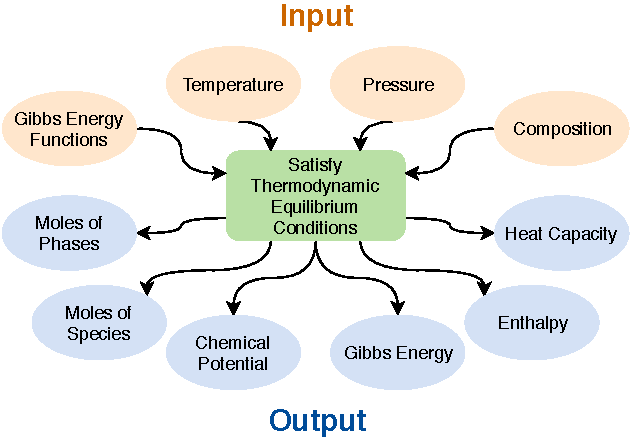
\includegraphics[width=0.75\textwidth]{figures/Thermodynamics.pdf}
        \caption{Input and output parameters of thermodynamic equilibrium calculations.}
        \label{fig:Thermodintro}
    \end{figure}
    
    Thermochemical equilibrium calculations are based on minimising the integral Gibbs energy of a closed system at constant temperature and hydrostatic pressure. From a numerical point of view, the objective of computing thermochemical equilibrium is to determine a unique combination of phases and their composition that yields a global minimum in the integral Gibbs energy subject to various linear and non-linear equality constraints. As shown in fig.~\ref{fig:Thermodintro}, by relying on the fundamental laws of thermodynamics, equilibrium computations use the system information, namely, Gibbs energy functions of the species that can be present in the system, temperature, pressure and composition to provide quantities such as the stable phases and species, Gibbs energy of the system, chemical potentials of the species and can be used to provide information such the enthalpy, heat capacity, etc. A detailed description of the thermodynamic equilibrium computation is provided in the following section.
    
    The thermochemical equilibrium solver in \texttt{Yellowjacket} leverages the experience from the development of a similar code \texttt{Thermochimica} \cite{Piro13}. By using the standard tools and libraries being used in \texttt{MOOSE}, the aim is to develop an improved thermochemical equilibrium solver for complete integration with other \texttt{MOOSE} based codes. This provides the foundation for future researchers to couple thermochemical simulations with fuel performance simulations in \texttt{Bison}, etc.
    	
\section*{Goals and Expected Outcomes}
The primary goal of this thesis is to develop a new state-of-the-art thermodynamic equilibrium code built on the \texttt{MOOSE} platform for direct coupling to \texttt{Marmot} for nuclear corrosion problems. Though the thermodynamic equilibrium code is being developed within the corrosion modelling application \texttt{Yellowjacket}, it could be easily coupled to other applications, such as the fuel performance code \texttt{Bison}. The code will rely on the \texttt{MOOSE} framework and exploit the multitude of mathematical and development tools of the framework to ensure that the code meets the stringent requirements of the nuclear industry. It must be mentioned that while \texttt{MOOSE} and other \texttt{MOOSE} based applications solve systems of partial differential equations (PDE) using the finite element method, the computational thermodynamics calculations are essentially  non-convex optimisation and require much more developmental effort than many other \texttt{MOOSE} applications where essentially just new PDEs need to be implemented.
	
	The anticipated major contributions of the work are as follows:
	\begin{enumerate}\compresslist
		\item Development of a new advanced Gibbs energy minimiser written in C++, built off \texttt{MOOSE}, and developed for multiscale, multiphysics simulations of nuclear materials.
		\item Full integration within the multiphysics framework \texttt{MOOSE} and direct coupling to 	\texttt{Marmot}.
		\item Enhanced initialisation algorithms to improve the computational performance.
		\item Investigation and implementation of robust global optimisation algorithms to increase reliability and performance.
		\item Software Quality Assurance with rigorous verification and testing to comply with the United States' NQA-1 guidelines required to be met for licensing.
	\end{enumerate}
	
\section*{Timeline}
The major research milestones are shown in the following table:
	\begin{table}[!htbp]
		\centering	
  		\begin{tabular}{@{}l r r@{}}
		\toprule
		\multicolumn{2}{c}{\textbf{Research Milestones}}\\
		\midrule
		\multicolumn{1}{c}{\textbf{Item}} & \multicolumn{1}{c}{\textbf{Timeline}} & \multicolumn{1}{c}{\textbf{Status}}\\
		\midrule
%		\multicolumn{2}{c}{\textbf{Coursework}}\\
%		\midrule
%		MCSC-6010G: Mathematical Modelling & Sep. - Dec. 2018 \\
%		MCSC-6030G: High Performance Computing & Sep. - Dec. 2018 \\
%		NUCL-6005G: Computational Thermodynamics [PhD level elective] & Sep. - Dec. 2018 \\
%		MCSC-6020G: Numerical Analysis & Sep. - Dec. 2019 \\
%		\midrule

%		\multicolumn{1}{c}{\textbf{Item}} & \multicolumn{1}{c}{\textbf{Timeline}}\\
%		\midrule
		Implement data file parsing code & Feb. - Mar. 2019 & Completed\\
		Implement linear solver (levelling) & Apr. - Jun. 2019 & Completed\\
		Implement non-linear solver for GEM (homogeneous) & Sep. 2019 - Mar. 2020 & In-progress\\
		Demonstration of non-linear solver capabilities & Mar. - May 2020 & Planned\\
		Begin integration of thermodynamic solver with phase field & Jun. - Aug. 2020 & Planned\\ 
		Implementation of global optimisation algorithm & Sep. 2020 - Mar. 2021 & Planned\\
		Demonstration of global optimisation capabilities & Apr. - May 2021 & Planned\\
		Complete integration of \texttt{Yellowjacket} into \texttt{MOOSE} & Jun. - Aug. 2021 & Planned\\
		Verification and testing & Sep. - Dec. 2021 & Planned\\
		\bottomrule
      		\end{tabular}
	\end{table}
	
\section*{Publication}
Following is a list of already published and soon to be submitted papers where contributions have been made as either primary author or co-author. The papers are attached in \nameref{publications}. 

\begin{enumerate}{\small
\item {M.\ Piro}, {M.\ Poschmann} and \textbf{P.\ Bajpai}, \textit{On the interpretation of chemical potentials computed from equilibrium thermodynamic codes: Applications to molten salts}, \href{https://doi.org/10.1016/j.jnucmat.2019.151756}{Journal of Nuclear Materials, 526 (2019) 151756}.
\item \textbf{P.\ Bajpai}, {M.\ Poschmann}, {M.\ Piro}, \textit{Derivations of useful partial molar excess Gibbs energy of mixing expressions of common thermodynamic models}, To be submitted to \href{https://www.journals.elsevier.com/calphad}{CALPHAD Computer Coupling of Phase Diagrams and Thermochemistry}. [In preparation]
\item \textbf{P.\ Bajpai}, {M.\ Poschmann}, {D.\ Andr\v{s}}, {C.\ Bhave}, {M.\ Tonks} and {M.\ Piro}, \textit{Development of a new thermochemistry solver for multiphysics simulations of nuclear materials}, \href{http://https://www.tms.org/TMS2020}{TMS 2020 Supplemental Proceedings, TMS 2020  - 149\textsuperscript{th} Annual Meeting \& Exhibition, San Diego, February 23-27, 2020}. [Accepted]
\item \textbf{P.\ Bajpai}, {M.\ Poschmann}, {D.\ Andr\v{s}} and {M.\ Piro}, \textit{Progress in developing a new thermochemistry code for corrosion modelling and multiphysics simulation of nuclear fuels}, \href{http://cns-annual-conference.org/2019/index.html}{39\textsuperscript{th} Annual Conference of the Canadian Nuclear Society and 43\textsuperscript{rd} Annual CNS/CNA Student Conference, Ottawa, June 23-26, 2019}.
}\end{enumerate}

In summary, with the aim of incorporating thermodynamic equilibrium calculations with the multiphysics simulation platform \texttt{MOOSE}, an advanced Gibbs energy minimiser is being developed as part of a the under development corrosion modelling tool \texttt{Yellowjacket}. Through advanced algorithm development and efficient implemetation of performance enhancing strategies, this research will focus on accelerating the performance of thermodynamic computations which are inherently very complex and can significantly impede the performance of multiphysics codes. A special focus will be on coupling to other \texttt{MOOSE} based codes and software quality assurance to comply with Nuclear Quality Assurance Level 1 standards. In the long run, the thermodynamic solver, and \texttt{Yellowjacket} in general, will support the development of advanced nuclear reactors.


%% The (optional) dedication can be used to thank someone or display a significant quotation.
 \dedication{\epigraph{This perpetual motion machine she made today is a joke, it just keeps going faster and faster... \\ Lisa ... In this house, we OBEY the laws of thermodynamics!}{Homer Simpson}}

%% Use Arabic numerals for the page numbers of the chapters.
\mainmatter

%% Turn on thumb indices.
%\thumbtrue


\chapter{Introduction} \label{chapter_1}

Recent years have seen a rapid shift in the engineering design of materials. Modelling and simulation have become essential tools in this context and are moving towards a multiscale, multiphysics approach where various physical phenomena  are coupled to enhance the accuracy of predictions. Of particular interest in this regard is the increasing desire to couple thermodynamics codes with other multiphysics codes such as phase field, fuel performance codes, etc. This chapter provides a brief background to the proposal and presents the motivation behind the proposed work.

\section{Introduction}
	Global population and per capita energy consumption are rising and electrical power generation not only plays a key role in the advancement of industry, agriculture, technology and the quality of living but is also an important measure of a country's economic development, power and independence. The global energy consumption has had significant impact on the environment in terms of greenhouse gas emissions and degradation of the quality of air, water and land.  As the call for action on climate change has become more pronounced and more urgent, there have also been concerns about energy security resource sustainability and human health. This has generated a renewed interest in nuclear energy as a source of reliable, low carbon footprint electricity source. 

	As of 2018, 450 nuclear plants around the world supplied 2563 TWh of electricity, around 10\% of the world's total electricity \cite{WNA:2019aa}. Despite the strong support for, and growth in, intermittent renewable electricity sources in recent years, the fossil fuel contribution to power generation has remained virtually unchanged in the last 10 years or so \cite{WNA:2019aa}. In its World Energy Outlook 2018, the Organisation for Economic Co-operation and Development (OECD) International Energy Agency (IEA)  has proposed an ambitious \emph{Sustainable Development Scenario} consistent with the provision of clean and reliable energy and a reduction of air pollution, among other aims. In this decarbonisation scenario, electricity generation from nuclear increases by almost 90\% by 2040 to 4960 TWh, and capacity grows to 678 GWe \cite{IEA:2018aa}. Meeting these goals not only requires committing to a continued operation of current nuclear power plants, but also rapid expansion and development of new nuclear plants. 
	
	Though many nations across the globe, both industrialised and developing, are confident of the potential of nuclear energy, challenges exist to future large scale use. These challenges relate to the sustainability, reliability and economic competitiveness, safety, risk of proliferation, anticipated future needs beyonds electricity, and need for government support \cite{GIF:2009aa}. To meet these challenges and develop future nuclear energy systems, the Generation {IV} International Forum (GIF) is undertaking necessary research and development to develop the next generation of innovative nuclear energy systems that can supplement today's nuclear plants and transition nuclear energy into the long term \cite{GIF:2019aa}. While promising in terms of sustainability, economics, safety and reliability, and proliferation resistance and physical protection, the Gen-{IV} nuclear reactors pose unique challenges in terms of engineering design, modelling and construction of these reactors. The design issues are themselves quite complicated and span a wide array of knowledge domains such reactor physics, chemistry, materials science, fluid flow and heat transfer, etc. Of particular interest and pertinent to this work are the material design issues discussed in the following section with a specific focus on corrosion.
	
\section{Modelling of Nuclear Materials}
	The environment in a nuclear reactor induces complex multiphysics phenomena in nuclear materials, occurring over distances ranging from inter-atomic spacing to meters, and times scales ranging from microseconds to years. This multiphysics behaviour is often tightly coupled and many important aspects are inherently multidimensional  \cite{WILLIAMSON2012149}. Once in the reactor, nuclear materials are subjected to extreme radiation environments that continuously alter their thermo-mechanical properties \cite{STAN200920}. Moreover, due to irradiation effects, the physics and chemistry of such materials become more complicated over time. The safe and reliable performance of nuclear power plants requires choice of suitable materials and the assessment of long-term materials damage.
	
	Modern materials, including nuclear materials are developed using a combination of discovery, which involves evaluating existing materials to identify candidates with desirable properties, and design, which aims at  creating new materials with predefined qualities \cite{STAN200920}. While the traditional approach to discovery and design of materials was almost entirely experimental, recent developments in modelling and high performance computing has resulted in a much stronger collaboration and integration among theory, experiments and computational science. Multiscale, multiphysics models and simulations enable investigations over  a wide range of length and time scales which would otherwise be unfeasible using only experiments. Thus, computational models help augment and guide experimental campaigns and support economical discovery and design of materials within reasonable lead times.  

	With material issues ranging from creep, swelling, fracture, fatigue to corrosion, impurity  effects and correlation between nano and microstructural scale, it is evident that a multiscale approach is required for a fundamental understanding of all the relevant phenomena. However, due to significant limitations on availability of computing resources, a majority of materials modelling and simulation efforts in the past adopted an operator splitting approach wherein the various physical phenomena were disconnected from each other. Though these methods were suitable for previous generation of nuclear reactors, addressing the materials challenges for advanced reactors requires a tightly coupled multiscale, multiphysics approach. 
	
	\begin{figure}[htbp]
		\centering
		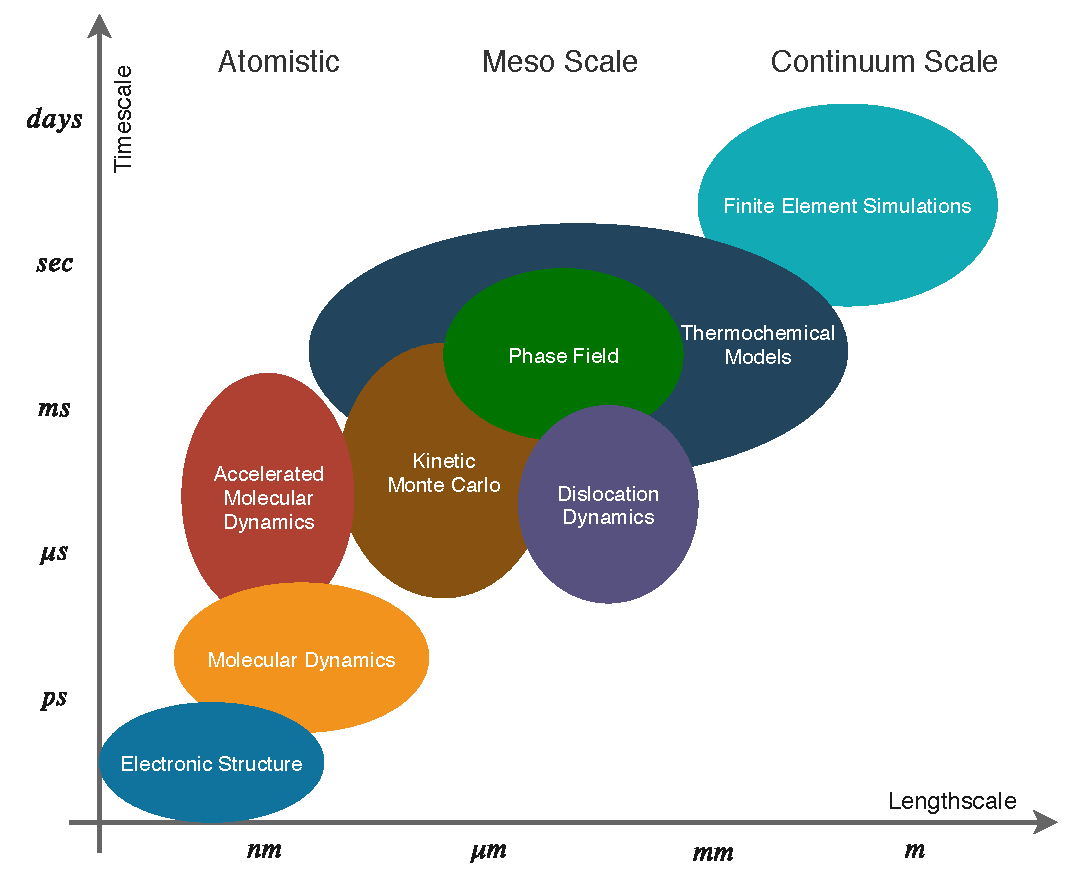
\includegraphics[width=0.75\textwidth]{figures/Multiphysics.pdf}
		\caption{Multiscale theoretical and computational methods used for materials model development and computer simulation \cite{STAN200920}.}
		\label{fig:multiphys}
	\end{figure}
	
	Traditionally, nuclear material modelling has focussed on the macroscale behaviour of the materials. Such models rely on the principles of thermo-mechanics and are heavily rooted in experimental observations. For example, nuclear fuel behaviour is often modelled as a solid mechanics problem coupled with conductive heat transfer and fission gas release wherein the material properties are often either assumed to be constant or described using simplified models based on empirical correlations. Recently, there has been an impetus on atomistically informing mesoscale  and macroscale methods by optimising characteristic parameters of these scales against the output of atomistic calculations \cite{STAN200920}. Since such an approach is rooted in fundamental principles, the transfer of information between scales, through characteristic parameters such as density, energy, temperature, etc., results in a much more accurate description of material behaviour. Some of the theoretical and computational methods used in multiscale approach have been shown in figure~\ref{fig:multiphys}.

	\subsection{Corrosion in materials}
	Many emerging nuclear technologies, such as the Molten Salt Reactors (MSR), use high temperature fluids, such as molten fluoride/chloride salts, which lead to corrosion of the metal containment leading to problematic behaviours during the reactor operations. Corrosion in molten salts is a fundamentally different process from that in conventional applications, and most of the methods to control corrosion developed over previous centuries are of limited value \cite{Yoshioka:2017aa}. In fluoride salts, the protective oxide layer on alloys typically relied upon for high-temperature corrosion resistance dissolves, thereby exposing the fresh alloy surface to the molten salt. In molten chloride salts, passivity has been observed; however, the oxide layer is prone to attack and may not provide the necessary corrosion protection \cite{Sridharan:2013aa}. The corrosion process is accelerated by the impurities present in the salt and enhanced further by the presence of dissimilar metals due to activity-driven corrosion. Another issue to be considered is the mass transfer of corrosion products from hotter sections of the nuclear reactor and subsequent deposition in the colder areas that can clog the heat exchanger systems. Therefore, effectively predicting corrosion and related phenomena like leaching and deposition requires a multiscale, multiphysics approach \cite{Mcmurray:2018aa}.
	
	Corrosion is an electrochemical process composed of oxidation and reduction reactions, which are defined by the thermodynamics and kinetics of the system. While thermodynamics controls whether or not a material may corrode, kinetics influences how quickly the material will corrode. This corrosion behaviour is also significantly affected by the material microstructure and predicting corrosion therefore requires a multiphysics approach that can couple quantitative electrochemistry models of corrosion and chemical reactions with thermochemical equilibrium computations.
	
	\subsection{Thermodynamic modelling of materials}
	The phase and chemical behaviour of nuclear materials is governed by the thermochemical equilibrium state. While in many systems, equilibrium is often not achieved due to transport and/or chemical kinetics phenomenon, a thorough understanding of both transport and chemical evolution, and subsequently material properties, is  based on an accurate representation of thermochemical equilibria \cite{Devanathan:2010aa}. As an example, the oxygen chemical potential acts as the driving force for transport of oxygen in oxide fuels but a determination of these chemical potentials is impossible without determining the stable phases which depends on the oxygen-to-metal ratio which in turn is a function of burnup.  In the specific context of corrosion modelling, the difference in the free energy of the salt fluoride/chloride constituents and the fluorides/chlorides of the alloying elements is a key driving force for corrosion. For closed systems, the equilibrium concentration of the corrosion product fluorides/chlorides in the salt melt dictates the maximum extent of corrosion and is important in the long-term corrosion of containment materials. Therefore, thermodynamic equilibrium calculations play an important role in the context of corrosion modelling in advanced reactors.
	
	Capturing thermodynamic equilibria in multiphysics codes has traditionally relied on empirical correlations and the interest in direct coupling of thermodynamic equilibrium codes with multiphysics model is only a recent trend. While the empirical correlations do not convey the high fidelity of original thermodynamic analysis, performing thermodynamic equilibrium analysis within multiphysics codes is normally a very complex process and can significantly impede the computational performance of such codes. However, the recent developments in high performance computing have enabled the incorporation of these calculations which are of ever more importance in the discovery and design of materials for advanced reactors. 
	
	The inputs for a thermodynamic equilibrium calculation are shown in figure~\ref{fig:Thermod}. Since thermodynamic equilibriums are isothermal and isobaric in nature, temperature and pressure are required as inputs along with the elemental composition of the material. While the equilibrium calculations are mathematically rigorous they do require thermodynamic models of materials to describe some parameters.  These thermodynamic models are generally developed using the Calculation of Phase Diagram (CALPHAD) approach shown in figure~\ref{fig:calphad}, which combines experimental and theoretical information to describe the thermodynamic properties through the Gibbs energy, applying a mathematical model containing adjustable parameters \cite{Lukas07}.  The multiscale approach also allows \textit{ab initio} molecular dynamics calculations to inform and improvise the thermodynamic models developed using the CALPHAD approach.
	\begin{figure}
        		\centering
        		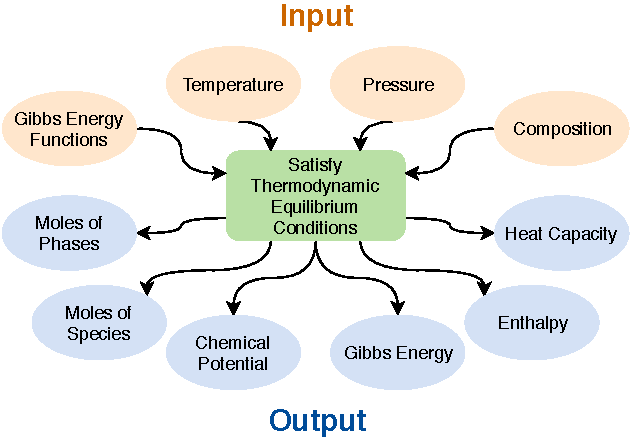
\includegraphics[width=0.75\textwidth]{figures/Thermodynamics.pdf}
        		\caption{Input and output parameters of thermodynamic equilibrium calculations.}
        		\label{fig:Thermod}
    	\end{figure}

Figure~\ref{fig:Thermod} also shows some of the outputs produced by thermodynamic equilibrium calculations. The main outputs include the phase assemblage, i.e. the number of moles of phases present at equilibrium and the mole fraction of the species in those phases. The equilibrium calculations also provide the Gibbs energy of the system, the chemical potentials of the species, etc. These quantities are useful in multiphysics calculations where, for example, the chemical potential of oxygen can be used to model oxygen diffusion in a \ce{UO2} nuclear fuel pellet.  
	\begin{figure}[htbp]
	\centering
	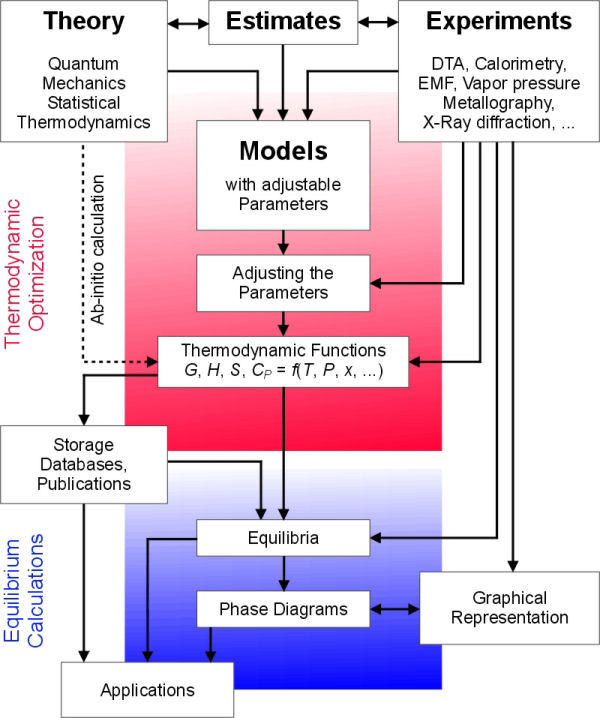
\includegraphics[width=0.5\textwidth]{figures/Calphad_method}
	\caption{Principle of CALPHAD method by Zinkevich \cite{Zinkevich:2003aa}}
	\label{fig:calphad}
	\end{figure}	

\section{Multiphysics Object Oriented Simulation Environment}
	The  Multiphysics Object-Oriented Simulation Environment \texttt{(MOOSE)} is a tool for solving complex coupled multiphysics equations using the finite element method. \texttt{MOOSE} uses an object-oriented design to abstract data structure management, parallelism, threading and compiling while providing an easy to use interface targeted at engineers that may not have a lot of software development experience. \texttt{MOOSE} provides extreme scalability and flexibility when compared to other finite element method (FEM) frameworks. For instance, \texttt{MOOSE} has the ability to run extremely complex material models, or even third-party applications within a parallel simulation without sacrificing parallelism. This capability is in contrast to what is often seen in commercial packages, where custom material models can limit the parallel scalability, forcing serial runs in the most severe cases \cite{gaston2015physics,moose-web-page}.

	The design goal of \texttt{MOOSE} is to give developers ultimate control over their physical models and applications. Designing new models or solving completely new classes of problems is accomplished by writing standard C++ source code within the framework's class hierarchy. Scientists and engineers are free to implement completely new algorithms using pieces of the framework where possible, and extending the framework's capabilities where it makes sense to do so. Commercial softwares do not have this capability, and instead opt for either a more rigid parameter system or a limited application-specific metalanguage \cite{moose-web-page}.
	
	Currently, apart from a number of other applications, such as \texttt{RELAP} \cite{Zhang:aa} for system level thermal hydraulics, \texttt{Rattlesnake} \cite{Wang:aa} for neutronics, etc., the \texttt{MOOSE} framework consists of two main applications for materials applications - the macroscale fuel performance code \texttt{Bison} \cite{Newman09} and the mesoscale phase field code \texttt{Marmot}  \cite{Tonks12}. Together, \texttt{MOOSE}, \texttt{Bison}  and \texttt{Marmot}, form the Fuels Product Line (FPL) to deliver an integrated set of increasingly predictive computational tools for nuclear fuel performance analysis and design. The FPL enable multiscale modelling and simulation of nuclear fuels where simulations of fuel performance at the engineering scale are informed by material property and behaviour models developed from mesoscale simulations of microstructure evolution under irradiation, which are themselves guided and enabled by inputs of fundamental materials parameters obtained from atomistic simulations. The multiscale, multiphysics approach allows an unprecedented degree of predictability of nuclear fuel performance.
	
	\subsection{Bison}
	The simulation of nuclear reactor fuel performance involves complex thermomechanical processes between fuel pellets, made of fissile material, and the protective cladding barrier that surrounds the pellets. \texttt{Bison} is an engineering scale code developed to predict the nuclear fuel performance under normal, off-normal, and accident conditions. By using highly efficient computational methods, \texttt{Bison} enables three dimensional, fully coupled multiphysics simulations on high fidelity geometric representations of fuel pins/pellets. \texttt{Bison} has been designed to be highly scalable and does not require the use of operator splitting, staggered or predictor-corrector approaches \cite{WILLIAMSON2012149}. 
	
	Within the multiscale framework, \texttt{Bison} can be coupled with both mesoscale microstructure evolution tool \texttt{Marmot} as well as reactor core and system tools being developed under the Reactor Products Line to perform full scale simulations of the entire nuclear reactor. Coupling with \texttt{Marmot} allows \texttt{Bison} to easily and continuously incorporate new mechanistic, physics-based models produced by the mesoscale model development activities in order to extend its predictive capability to new fuels and operational regimes. While focussed on Light Water reactor (LWR) fuel, \texttt{Bison} is applicable to variety of fuel forms including the spherical TRISO fuel design \cite{NEAMS}. 
	
	\subsection{Marmot}
	Due to its simple concept and large range of applicability, the phase field approach is a popular and powerful tool to model microstructure and has been applied in problems such as grain boundary migrations, martinistic transformation, two-phase flow, etc. The phase field approach treats all material interfaces as diffuse by representing structural features with continuous variables which smoothly transition from one value to another. Thus, phase field method not only eliminates the need to explicitly discretise boundaries and interfaces, it also enables describing microstructure through a system of partial differential equations.  The \texttt{Marmot} phase field framework has been developed to enable simulations of the microstructure evolution of nuclear fuels and materials under irradiation. By exploiting the object-oriented architecture of \texttt{MOOSE}, \texttt{Marmot} allows easy coupling of phase field with additional physics such as solid mechanics or heat conduction, to effectively predict the microstructural evolution at mesoscale. This allows prediction of evolution of material properties of nuclear materials under irradiation and can be used to inform engineering scale simulations and reduce the dependence of such simulations on empirical correlations. As a result, the multiscale framework can achieve true predictability even in compositional and operational regimes where little or no experimental data exists.
	
	Despite the wide ranging capabilities of the FPL, there remains a gap in terms of modelling advanced nuclear reactors. The high temperature operations of reactors such as the Molten Salt Reactors (MSR), which use molten fluoride/chloride salts as the fuel and coolant, produce a conducive environment for corrosion. The current FPL lacks a tool for corrosion modelling at microstructure scale and efforts are underway to develop a new \texttt{MOOSE} based application called \texttt{Yellowjacket} to bridge this gap. 

	\subsection{Yellowjacket}	
	\texttt{Yellowjacket} is a mesoscale framework for thermodynamics based modelling of corrosion in advanced reactor materials. Currently under development, it is a \texttt{MOOSE} based application that couples quantitative models of corrosion with thermodynamic equilibrium and chemical kinetics models to predict the rate of material loss, corrosion product production and precipitate production in advanced nuclear reactors. \texttt{Yellowjacket} relies on phase field models for structure evolution, coupling it with Poisson equation for electrostatics, fracture models and thermochemical equilibrium solvers to provide a holistic environment for corrosion modelling and simulation. As shown in figure~\ref{fig:yjmoose}, \texttt{Yellowjacket} depends on the \texttt{MOOSE} framework for the development infrastructure and follows the Nuclear Quality Assurance Level 1 (NQA 1) \cite{NQA-web-page} development process. 
	
	\begin{figure}[htbp]
		\centering
		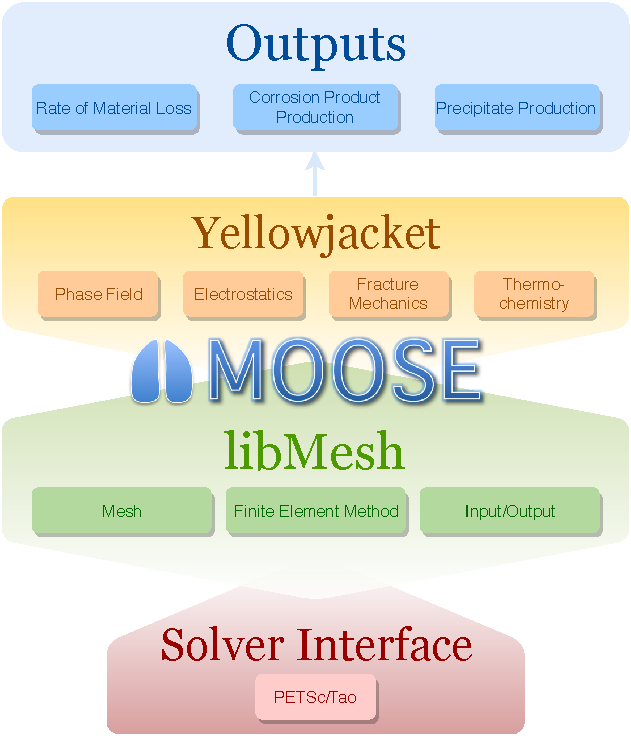
\includegraphics[width=0.75\textwidth]{figures/Yellowjacket_MOOSE.pdf}
		\caption{Illustration showing the underlying interface provided by \texttt{MOOSE} and the physics modules of \texttt{Yellowjacket}.}
		\label{fig:yjmoose}
	\end{figure}
	
	\texttt{Yellowjacket} is being developed through a joint collaboration between the Nuclear Fuels and Materials Group at Ontario Tech University, University of Florida, Idaho National Laboratory and Los Alamos National Laboratory, and is funded primarily by the United States Department of Energy (US-DOE) through the Nuclear Energy Advanced Modelling and Simulation (NEAMS) program.  
	
	This thesis is aimed at developing a thermodynamic equilibrium solver for the corrosion modelling tool \texttt{Yellowjacket} and the goals of this research are specified in the following chapter. The phase field component of \texttt{Yellowjacket} is being investigated by another PhD student at University of Florida.
	

	

\chapter{Goals of Research} \label{chapter_2}

	Facilitating the discovery and design of nuclear materials for innovative nuclear materials requires use of multiscale, multiphysics models and simulations and chemical thermodynamics forms an integral part of such simulations. The motivation behind this research is to directly integrate thermodynamic equilibrium computations in the Multiphysics Object Oriented Simulation Environment (\texttt{MOOSE}) which is a generic finite element method based simulation framework. By computing various thermodynamic values on a finite element mesh and using these values to inform macroscale and mesoscale models, an unprecedented level of sophistication can be achieved in multiscale, multiphysics models for materials.  

	Some of the challenges in achieving this objective include computational expense, predictive capabilities and reliability. First, relatively limited capabilities are currently available to perform such coupling. Within the \texttt{MOOSE} framework, the thermodynamic equilibrium code \texttt{Thermochimica} has only recently been integrated with the macroscale code \texttt{Bison} while the mesoscale code \texttt{Marmot} still relies on empirical correlations for thermodynamic inputs and coupling \texttt{Thermochimica} with it would require starting the process of coupling for scratch.  Second, the computational expense of thermodynamic equilibrium dramatically increases the computational burden of the multiphysics simulations. Finally, reliability is of utmost importance for simulation of nuclear materials and requires an enormous number of function evaluations. 
	
	While there are a number of existing thermodynamic equilibrium tools, all but a handful of them are standalone codes and since computational time for such computations is not of high importance, there has been no interest in optimising their performance. In order to maintain numerical stability, most of the codes restrict the number of system components but the intended application also requires that the new code be able to handle systems with a very large number of components. Another issue that needs to be addressed is the challenge associated with initialisation algorithms for the code. A far from accurate initial estimate can significantly reduce the convergence rate impeding the performance of the simulations and the current schemes used for initialisation often increase the computational cost when used at every iteration in the multiphysics simulations. Finally, the convergence of solution to the true solution and not a false positive must be ensured which requires the use of global optimisation methods. 
  
	The goal of this work is to develop a new state-of-the-art thermodynamic equilibrium code by leveraging the experience with the development and utilisation of \texttt{Thermochimica}. Though the thermodynamic equilibrium code is being developed within the corrosion modelling tool \texttt{Yellowjacket}, it would be easily couple-able with other applications such as \texttt{Bison} and \texttt{Rattlesnake}. The code will rely on the \texttt{MOOSE} framework and exploit the multitude of mathematical and development tools of the framework to ensure that the code meets the stringent requirements of the nuclear industry. It must be mentioned that while \texttt{MOOSE} and other \texttt{MOOSE} based applications solve systems of partial differential equations (PDE) using finite element method, thermodynamic equilibrium calculation is essentially a non-convex optimisation problem and requires much more developmental effort than many other \texttt{MOOSE} applications where essentially just new PDEs need to be implemented.
	
	The major contributions of the work would be as follows:
	\begin{enumerate}
		\item Development of a new advanced Gibbs energy minimiser written in C++ within the framework of \texttt{MOOSE} platform.
		\item Full integration within the multiphysics framework \texttt{MOOSE}, with the intent of coupling to the phase field code \texttt{Marmot}\footnote{The phase field module development and coupling is being investigated at University of Florida.}. 
		\item Enhanced initialisation algorithms to improve the computational performance.
		\item Investigation and implementation of robust global optimisation schemes to increase reliability and robustness.
		\item Software Quality Assurance  with rigorous verification and testing to comply with the NQA-1 guidelines required to be met for licensing.
	\end{enumerate}




\chapter{Thermodynamic Basis} \label{chap:thermo}

The laws that govern all material systems can be expressed in two seemingly simple statements of Rudolf Clausius - \emph{``Die Energie der Welt ist konstant. Die Entropie der Welt strebt einem Maximum zu.''} and yet thermodynamics has drawn the attention of many great scientists including Maxwell, Boltzmann, Planck and  Mach. Physicist Arnold Sommerfeld accounted his experience of thermodynamics as \emph{``Thermodynamics is a funny subject. The first time you go through it, you don't understand it at all. The second time you go through it, you think you understand it, except for one or two small points. The third time you go through it, you know you don't understand it, but by that time you are so used to it, it doesn't bother you any more''}. A number of definitions and laws of thermodynamics form the basis of equilibrium thermodynamics and the Gibbs energy models and equations play a key role in the structure of the equilibrium solver.

%==============================================================================================================================
%															Definitions
%==============================================================================================================================
%\section{Definitions}
%

%==============================================================================================================================
%														Laws of Thermodynamics
%==============================================================================================================================
\section{Fundamental Laws of Thermodynamics}
	The statements of Rudolf Clausius are now known as the \emph{First and Second Laws of Thermodynamics}. Before looking at these laws, the basic definitions used in subsequent sections are reviewed for clarity. A \emph{thermodynamic system} is a portion of the universe with a perimeter defined by real or imaginary boundaries and usually consists of many chemical components whose thermodynamic behaviour can be analysed. For example, the volume element shown in figure~\ref{fig:system} can be treated as a thermodynamic system. A system that may exchange matter with its system boundary is called \emph{open} while a system that can only exchange energy and not matter is called \emph{closed}. The term \emph{isolated} is used for a system that is cut off from the surroundings and can neither exchange matter nor energy. In material thermodynamics, the system is often treated as closed, notable exceptions being chemical reactors where reactants and products continuously flow in and out of the system.
 	\begin{figure}[htb]
		\centering
		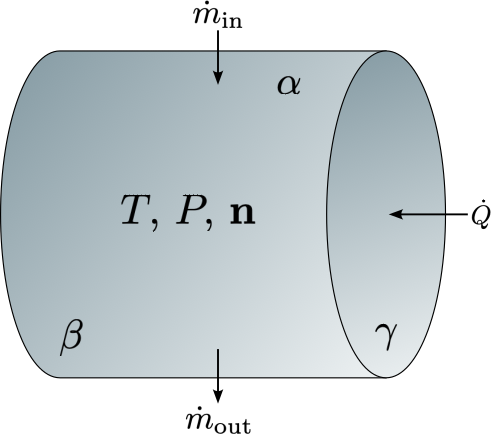
\includegraphics[width=0.45\textwidth]{figures/chapter-3/system.png}
		\caption{Volume element of a general thermodynamic system with mass flow of chemical components $\dot{m}$ and heat flux $\dot{Q}$. The Greek letters indicate presence of separate phases.}
		\label{fig:system}
	\end{figure}

	A thermodynamic system can be described macroscopically using \emph{state variables}, which are represented by measurable macroscopic quantities such as temperature, pressure, volume, amounts of different substances, etc. \emph{Intensive variables} (e.g. temperature and pressure)  are independent of the amount of matter in the system  while  \emph{extensive variables} (e.g. volume and total internal energy) are dependent on the mass of the system.  With a change in the internal variables, the system undergoes a change in state. If a system can be restored to the original condition without any change in the state of the surroundings, the process through which the state of the system was changes is described as a \emph{reversible process}. However, all real processes are \emph{irreversible processes}, that is, the system cannot be recycled.

	Thermodynamics concerns the state of a system as it interacts with its surroundings and is based on two physical laws: the first and second laws of thermodynamics. The first law of thermodynamics describes those interactions, which can involve exchanges of any combinations of heat, work, and mass, while the second law of thermodynamics governs the evolution of state inside the system. Together, the two laws integrate the external and internal parts of the system.

	\subsection{First law of thermodynamics}
	The first statement of Clausius and what is now known as the first law of thermodynamics expresses the conservation of energy\footnote{Considering Einstein's mass-energy equivalency, the classical first law can be modified to state that mass and energy together are constant. However, since we are considering chemical equilibrium and not dealing with nuclear reactions, the classical form of first law applies.} and is formulated as follows:

		\hangindent=\parindent \emph{Energy cannot be created or destroyed, and the energy increase of a system ($dU$) equals the sum of the heat absorbed from the surroundings ($dQ$) and the work ($dW$) done by the surroundings on the system.}

	\noindent Mathematically, for an open system, the first law can be expressed as:
	\begin{equation}\label{eqn:flot}
		dU = dQ + dW + \sum H_i dN_i,
	\end{equation}
	where $dN_i$ denotes the amount of component $i$ exchanged with the surroundings and $H_i$ is the unit energy of component $i$ in the surroundings, and the summation is for all the independent components in the system. Since the systems of interest in thermodynamics of materials are closed, there is no exchange of matter between the system and the surroundings and the first law of thermodynamics takes the following form:
	\begin{equation}\label{eqn:flot1}
		dU = dQ + dW,
	\end{equation}
	where both $dQ$ and $dW$ depend on the thermodynamic process and hence do not qualify as state functions.

	\subsection{Second law of thermodynamics}
	In 1850, Clausius formulated a criterion for the direction of spontaneous processes and called it \emph{entropy}. His second statement translates to entropy of the universe tends to maximum and is now known as the second law of thermodynamics. Formally, the second law states that:

	\hangindent=\parindent \emph{For an internal process to take place spontaneously, or irreversibly, the change in entropy of the system ($dS$) must be positive.}

	\noindent In mathematical form, the second law can be formulated as:
	\begin{equation}\label{eqn:slot}
		dS = dS_\text{sys} + dS_\text{surr} \geq 0,
	\end{equation}
	where the $S_\text{sys}$ and $S_\text{surr}$ represents the entropy of the system and surroundings respectively.
	In the course of a reversible, isothermal process, the entropy change of the system $dS_\text{sys}$   can be defined as the heat exchange divided by temperature:
	\begin{equation}\label{eqn:slotrev}
		dS_\text{sys} = \frac{dQ}{T}.
	\end{equation}

	\subsection{Third law of thermodynamics}
	The third law of thermodynamics allows expressing the absolute value of the entropy in contrast to the internal energy by assigning an entropy equal to zero at \SI{0}{\kelvin} for any pure compound in stable and perfectly crystalline state.

%==============================================================================================================================
%												Enthalpy, and Helmholtz and Gibbs Energies
%==============================================================================================================================
\section{Enthalpy, and Helmholtz and Gibbs Energies}
		Three important state functions of great practical importance in thermodynamics are the \emph{enthalpy} $H$, \emph{Helmholtz energy} $F$, and \emph{Gibbs energy} $G$. Enthalpy changes are of importance in calorimetry experiments as they can be directly measured while Helmholtz and Gibbs energies are used in defining chemical equilibrium conditions.

		The enthalpy of a thermodynamic system is an extensive property defined as:
		\begin{equation}
			H = U + PV,
		\end{equation}
		where $U$ denotes the internal energy, $P$ denotes the pressure the system is at and $V$ represents the volume of the system.

		The Helmholtz energy of a thermodynamic system is defined as:
		\begin{equation}
			F = U - TS,
		\end{equation}
		where, $T$ denotes the absolute temperature of the system and $S$ represents the entropy of the system.

		The Gibbs energy of a thermodynamic system is defined as:
		\begin{equation}
			G = H - TS.
		\end{equation}

		The equilibrium criterion can be derived in terms of Helmholtz and Gibbs energies. According to the second law of thermodynamics, a spontaneous irreversible process must be accompanied by an overall positive change of entropy, i.e.:
		\begin{equation}
			dS_\text{sys} + dS_\text{surr} > 0.
		\end{equation}
		For a closed system in thermal and mechanical equilibrium but not in chemical equilibrium which acquires an infinitesimal quantity of heat from the surroundings:
		\begin{equation}
			dS_\text{surr} = -\frac{dQ_\text{sys}}{T},
		\end{equation}
		where it is assumed that the mass of the surroundings is large enough so that addition/removal of the heat does not cause a perceptible change in temperature. Thus,
		\begin{equation}
			{dQ_\text{sys}} - T dS_\text{sys}  < 0.
		\end{equation}

		Assuming that the heat exchange causes an infinitesimal change in the internal energy of the system by an amount $dU_\text{sys}$, according to the first law of thermodynamics,
		\begin{equation}
			{dU_\text{sys}} = {dQ_\text{sys}} + {dW_\text{sys}}.
		\end{equation}

		For a closed, isobaric system the work is purely due to the change in the volume of the system and the following relationship is obtained:
		\begin{equation}
			{dU_\text{sys}} + P{dV_\text{sys}} - T{dS_\text{sys}} < 0.
		\end{equation}

		If both the temperature and volume were held constant, the above inequality becomes:
		\begin{equation}
			d{U_\text{sys} - TS_\text{sys} } < 0.
		\end{equation}

		Since the terms within the parentheses denote the Helmholtz energy, one obtains the criterion for spontaneous change of isothermal, isochoric system, which is expressed as:
		\begin{equation}
			d{F_\text{sys} } < 0
		\end{equation}

		Similarly, if the temperature and pressure were held constant, the inequality becomes:
		\begin{equation}
			d{U_\text{sys} + PV_\text{sys} - TS_\text{sys} } < 0.
		\end{equation}

		The terms inside the parentheses denote the Gibbs energy and subsequently yield the criterion for spontaneous change of an isothermal, isobaric system:
		\begin{equation}
			d{G_\text{sys} } < 0.
		\end{equation}

		Thus, for the equilibrium of a closed system at constant temperature and volume, it is necessary and sufficient that the Helmholtz energy of the system is at minimum and equivalently, the Gibbs energy of the system must be at minimum for equilibrium in systems at constant temperature and pressure. In equilibrium thermodynamics, Gibbs energy is often preferred over Helmholtz energy since controlling pressure is easier than controlling volume during experiments. It must be emphasised that thermodynamic properties are fundamentally concerned with relative changes, a property that is often exploited in computations.

%==============================================================================================================================
%												Gibbs Energy and Chemical Potential
%==============================================================================================================================
\section{Gibbs Energy and Chemical Potential}
	Of particular interest in description of  thermodynamic equilibrium are the quantities named \emph{potentials}. A system is in thermodynamic equilibrium when it is simultaneously in thermal, mechanical, electrical and chemical equilibrium. This also refers to the state where there are no unbalanced potentials within the system. J.W. Gibbs used the term \emph{thermodynamic potential} to represent all the relevant system potentials to characterise the conditions of thermodynamic equilibrium \cite{Gibbs:1878aa}. Thermodynamic equilibrium calculations are based on the principle that the potential for each component must be uniform throughout the system at thermodynamic equilibrium. This section and the following describe the relation between Gibbs energy and chemical potentials and their use in computing thermodynamic equilibrium.

	The Gibbs energy, $G_{i}$ [\si{\joule \per \mole}], of a pure species  $i$ is defined as \cite{Zemansky81}:
	\begin{equation} \label{eqn:Gibbs_der1}
			G_{i} = \Delta H_{i} - TS_{i},
	\end{equation}
	where T [\si{\kelvin}] is the absolute temperature, $\Delta H_{i}$ [\si{\joule \per \mole}] and $S_{i}$ [\si{\joule \per \mole \per \kelvin}] represent the enthalpy and absolute entropy of species $i$ in phase $\phi$ respectively. Since thermodynamic quantities are relative in nature, equation ~\eqref{eqn:Gibbs_der1} can be expanded as:
	\begin{equation} \label{eqn:Gibbs_der2}
			G_{i} = \left(\Delta H_{i}^\circ + \int_{T_0}^{T} C_{p,i}dT \right) - T\left( S_{i}^\circ  + \int_{T_0}^{T} \frac{C_{p,i}}{T}dT \right) + \int_{P_0}^{P} V_i dP,
	\end{equation}
	where $\Delta H_{i^\circ}$ [\si{\joule \per \mole}] and $S_{i^\circ}$ [\si{\joule \per \mole \per \kelvin}] are the standard enthalpy of formation and entropy respectively at standard temperature ($T_0 = 298.15$ \si{\kelvin}) and pressure ($P_0 = 1$ \si{atm}). The superscript / subscript $\circ$ represents a quantity at standard temperature and pressure, a notation that is used hereafter. $C_{p,i}$ [\si{\joule \per \mole \per \kelvin}]  denotes the molar heat capacity at constant pressure, $P$ [\si{atm}] is the absolute pressure and $V_i$ [\si{\meter \cubed \per \mole}] denotes the molar volume. For an ideal gas, from the gas law, the last term in equation~\eqref{eqn:Gibbs_der2} can be written as $RT \ln{\left(P/P_0\right)}$, where $R = 8.314462$ [\si{\joule \per \mole \per \kelvin}] is the ideal gas constant. For a pure ideal gas species $i$, the standard Gibbs energy is:
	\begin{equation} \label{eqn:Gibbs_der_id}
			G_{i} = \left(\Delta H_{i}^\circ + \int_{T_0}^{T} C_{p,i}dT \right) - T\left( S_{i}^\circ  + \int_{T_0}^{T} \frac{C_{p,i}}.{T}dT  - R \ln{\left(\frac{P}{P_0}\right)}\right).
	\end{equation}

	The fact that Gibbs energies are relative quantities and can be numerically adjusted as long as the elemental differences are preserved is of practical importance and is often used in thermodynamic equilibrium calculation. Chemical potential of species $i$ in phase $\lambda$, $\mu_{i(\lambda)}$ [\si{\joule \per \mole}], is a measure of the change of the Gibbs energy of the system by the introduction of species $i$ and incorporates  the reference Gibbs energy of pure species, $g_{i}^\circ$, and the entropic contribution due to mixing as a function of its mole fraction. Mathematically, the chemical potential of a species $i$ is defined as \cite{Zemansky81}:
    	\begin{equation}\label{eq:mu_def}
        		\mu_{i} = {\left (\frac{\partial G_\text{sys}}{\partial n_{i}} \right )}_{T,P,n_{j \neq i}}.
    	\end{equation}

	For the species of a phase with only ideal mixing, the chemical potential is generally given as:
    	\begin{equation}
        		\mu_{i} = g_{i}^\circ + \ln x_{i}.
    	\end{equation}

	For non-ideal solution phases, the chemical potential also includes the partial molar excess Gibbs energy of mixing, $g_{i}^{ex}$ [\si{\joule \per \mole}], to account for non-ideal mixing as follows:
    	\begin{equation}\label{eq:mu_ex}
        		\mu_{i} = \mu_{i}^\circ + \ln x_{i} + \mu_{i}^{ex}.
    	\end{equation}

    	While the chemical potential of stoichiometric phases does not include a composition dependent term, the partial molar excess Gibbs energies of mixing for non-ideal solution models depend on the mixing model employed. Some of these models include the Modified Quasichemical Model \cite{Pelton00,Pelton01,Chartrand01,Pelton01b,Lambotte11}, the Compound Energy Formalism \cite{Hillert01}, etc.

	The integral Gibbs energy of a multicomponent, multiphase system is represented as:
	\begin{equation}\label{eqn:integralGibbs1}
        		G_\text{sys} = RT \left ( \sum_{\phi=1}^{\Phi} n_{\phi} \sum_{i=1}^{N_{\phi}}x_{i}\tilde{\mu}_i \right ),
    	\end{equation}
	where $R$ [\si{\joule \per \mole \per \kelvin}] is the ideal gas constant, $T$ [\si{\kelvin}] is the absolute temperature, $N_{\phi}$ denotes the number of species in phase $\phi$ of which there can be a maximum of $\Phi$ and $x_{i}$ represents the mole fraction of species $i$. For convenience, the Gibbs energy is often split into separates contributions from solution and stoichiometric phases as follows:
    	\begin{equation}\label{eqn:integralGibbs}
        		G_\text{sys} = RT \left ( \sum_{\lambda=1}^{\Lambda} n_{\lambda} \sum_{i=1}^{N_{\lambda}}x_{i}\tilde{\mu}_i + \sum_{\omega=1}^{\Omega} n_{\omega} \tilde{\mu}_{\omega} \right ),
    	\end{equation}
    	$N_{\lambda}$ denotes the number of species in the solution phase $\lambda$ and $x_{i}$ represents the mole fraction of species $i$ in solution phase $\lambda$. $\Lambda$ and $\Omega$ represent the number of stable solution phases and stoichiometric phases, respectively, and the number of moles of the solution phase $\lambda$ and stoichiometric phase $\omega$ are denoted by $n_\lambda$ and $n_\omega$ [\si{\mole}], respectively. $\tilde{\mu_i}$ represents the dimensionless form of the chemical potential of species $i$ and is given as $\tilde{\mu}_i = \mu_i / RT$\footnote{The dimensionless form $\tilde{\mu}_i$ has been used here as it is the preferred form in computational implementations.}. Finally, $\tilde{\mu}_i$ and $\tilde{\mu}_\omega$ represent the dimensionless chemical potential of species $i$ in solution phase $\lambda$ and stoichiometric phase $\omega$ respectively.

	The Gibbs energy of  the system can also be expressed in terms of the element potentials, $\Gamma_j$ [\si{\joule \per \mole}], and the number of moles, $b_j$ [\si{\joule}], of the system components. Mathematically, this can be expressed as:
	\begin{equation}\label{eq:elempot}
        		G_\text{sys} = \sum_{j=1}^{C} \Gamma_j b_j,
    	\end{equation}
	where $C$ denotes the number of system components which is normally the number of elements in the system. The mixing models used in materials modelling are briefly described in the following section.

	\subsection{Excess mixing models for Gibbs energy}
	A number of different models for excess mixing component of Gibbs energy have been proposed in literature. The different models are suitable for different materials, for example the Compound Energy Formalism (CEF) is often used for \ce{UO2} fuels while the Modified Quasichemical Model (MQM) is the state of the art model used to describe molten salts, which are of prime interest in the development of MSRs. However, only the relevant equations for some of the most commonly used models are shown here.
	\begin{enumerate}
	\item \textbf{Substitutional solution models}\\
	The regular solution model is a quantitative explanation of non-ideal behaviour. The model assumes that the entropy of mixing is the same as ideal mixing but that the enthalpy of mixing is not zero. A number of different regular solution models have been proposed, the most commonly used ones being based on Kohler-Toop and Redlich-Kister-Muggiano interpolation schemes \cite{Lukas07}.
		\begin{itemize}
			\item \textbf{Kohler-Toop Interpolation}
			\begin{equation}
				g_{\lambda}^\text{ex} = \sum_{z=1}^Z \phi_z (x_1^{d_1} x_2^{d_2} x_3^{d_3} ).
			\end{equation}
			\item \textbf{Redlich-Kister-Muggiano Interpolation}
			\begin{equation}
				g_{\lambda}^\text{ex} = \sum_{z=1}^Z x_j x_k \sum_{\nu = 0} {^\nu}L_{j}.
			\end{equation}
			\end{itemize}
	\item \textbf{Compound Energy Formalism (CEF)} \\
	Compound Energy Formalism is a multi-sublattice model proposed by Hillert \cite{Hillert01} for an adequate description of the properties of solution phases with sublattices. The molar Gibbs energy, $g_{\lambda}$, of solution phase $\lambda$ based on the CEF model is generally given as:
	\begin{equation}\label{eq:g_lambda}
	g_{\lambda} = \sum_{i=1}^{N_{\lambda}} g_{i}^{\circ} \prod _{s=1}^{N_s} y_{i(s)} + RT\left( \sum_{s=1}^{N_s} a_s \sum_{c=1}^{N_c}   y_{c(s)} \mathrm{ln} (y_{c(s)}) \right) + g_{\lambda}^\text{ex},
	\end{equation}
	where $g_{i}^{\circ}$ is the standard molar Gibbs energy of the pure component $i$,
$y_{i(s)}$ represents the site fraction on sublattice $s$ corresponding to component $i$, $N_{\lambda}$ and
$N_s$ denote the number of components and number of sublattices in solution phase $\lambda$, respectively.
The ideal gas constant is represented by $R$, the absolute temperature by $T$, the stoichiometry
coefficient for sublattice $s$ is represented by $a_s$, the number of constituents on sublattice $s$ is $N_c$
and the site fraction of constituent $c$ on sublattice $s$ is $y_{c(s)}$.  It is to be understood that $y_{i(s)}$
refers to the site fraction of  constituent $c$ associated with component $i$ on sublattice $s$ and is thus
related to $y_{c(s)}$.  Finally, the molar excess Gibbs energy of mixing of solution phase $\lambda$ is
$g_{\lambda}^\text{ex}$ and is given as:
\begin{equation}
	\label{eq:g_ex}
	g_{\lambda}^\text{ex} = 	 \sum_{p=1}^{N_p} \left( \prod_{m=1} y_{m(s)}  \right)   \sum_{z=0}^{N_z} {^zL_{j,k}} (y_j - y_k)^{z},
\end{equation}
where $N_p$ denotes the number of excess mixing parameters (note: $N_p \ge N_s$), $y_m$ is the site fraction of constituent $m$ corresponding to mixing parameter $p$, $N_z$ is the number of terms corresponding to parameter $p$,  and ${^zL_{j,k}}$ is the $z$th order mixing parameter. A detailed description of CEF can be found in the paper by Hillert \cite{Hillert01}.
	\item \textbf{Modified Quasichemical Model (MQM)} \\
	The Modified Quasichemical Model (MQM) in the quadruplet approximation is the most generalised thermodynamic model for treating Short Range Ordering (SRO). MQM is fundamentally different than other thermodynamic models in that the focus is not on the mixing of chemical species or constituents on a lattice, but rather the mixing of species as quadruplets to capture SRO of both First Nearest Neighbour (FNN) and Second Nearest Neighbour (SNN) in liquid or solid solutions. The details of evolution of MQM from pair approximation for species mixing on only one sublattice to the current quadruplet approximation are provided by Pelton \textit{et al.} \cite{Pelton00,Pelton01,Chartrand01,Pelton01b}.

        For a solution with two sublattices, which is occupied only by a single species on the second sublattice, the SNN pair exchange can be written as:
            \begin{equation} \label{SNNPairExchange1}
	            (A-[X]-A) + (B-[X]-B) = 2(A-[X]-B); \Delta g_{AB/X},
            \end{equation}
        where $\Delta g_{AB/X}$ is the non-configurational Gibbs energy for the formation of 2 mol of $(A-[X]-B)$ pairs. Similarly, when there is a single species on the first sublattice, the formation of SNN pairs is captured via:
            \begin{equation} \label{SNNPairExchange2}
	            (X-[A]-X) + (Y-[A]-Y) = 2(X-[A]-Y); \Delta g_{A/XY}
            \end{equation}
        where $\Delta g_{A/XY}$ is the non-configurational Gibbs energy for the formation of 2 mol of $(X-[A]-Y)$ pairs.
        Among the FNN pairs, the following exchange reaction is considered:
            \begin{equation} \label{FNNPairExchange}
	            (A-X) + (B-Y) = (A-Y) + (B-X); \Delta g_{A/XY}^\text{exchange}
            \end{equation}
        where $\Delta g_{A/XY}^\text{exchange}$ is the non-configurational Gibbs energy.
        Let $n_i \; (i=A,B,...,X,Y...)$ represent the number of moles of species $i$, $n_{i/j}$ be the number of moles of FNN ($(i - j)$) pairs, and $n_{ij/kl}$ be the number of moles of the quadruplets. The relationship between the foregoing terms is \cite{Pelton01b}
        \begin{gather}\label{EqMassBalance1}
	       Z_A n_A  = 2n_{A_2/X_2} + 2n_{A_2/Y_2} + 2n_{A_2/XY} + n_{AB/X_2} + n_{AB/Y_2} + n_{AB/XY} + \cdots, \\
	       Z_X n_X  = 2n_{A_2/X_2} + 2n_{B_2/X_2} + 2n_{AB/X_2} + n_{A_2/XY} + n_{B_2/XY} + n_{AB/XY} + \cdots,
        \end{gather}
        where $Z_A$ and $Z_B$ are the coordination numbers for A and B, respectively. A generic statement for a multi-component system is:
  	\begin{equation}
		Z_i n_i = 2n_{ii} + \sum_{j \ne i} n_{ij}.
         \end{equation}
        The mole fractions then follow:
        \begin{gather} \label{EqMoleFraction}
            x_{i} = \frac{n_{i}}{\sum n_j}, \\
            x_{k} = \frac{n_{k}}{\sum n_l},
        \end{gather}
        where the indices $i$ and $j$ refer to the species on first sublattice while the indices $k$ and $l$ refer to the species on second sublattice.
        The FNN pair fractions and quadruplet fractions are defined as:
        \begin{gather} \label{EqPairFraction}
            x_{i/k} = \frac{n_{i/k}}{\sum_j \sum_l n_{j/l}}, \\
            x_{ij/kl} = \frac{n_{ij/kl}}{\sum n_{ij/kl}}.
        \end{gather}
        Another useful term is the coordination equivalent fraction, which is
            \begin{gather} \label{EqCoordEqFraction}
	            y_i = \frac{Z_i n_i}{\sum Z_j n_j}, \\
	            y_k = \frac{Z_k n_k}{\sum Z_l n_l}.
            \end{gather}
	\end{enumerate}
	Omitting detailed description of the derivation of the model, the simplest form of MQM for binary solutions can be written as:
	\begin{equation} \label{EqGibbsMQM1}
		G_{\lambda} = (n_A g_A^\circ + n_B g_B^\circ) - T\Delta S^\text{config} + \frac{n_{AB} \Delta g_{AB}}{2}
	\end{equation}
	where $g_i^\circ$ is the reference molar Gibbs energy of pure $i$ (computed from a database), $T$ is the absolute temperature, and $\Delta S^\text{config}$ is the configurational entropy, given by:
	\begin{multline} \label{EqConfigEntropy}
		\Delta S^\text{config} = -R\left( n_A \ln(x_A) + n_B \ln(x_B) \right . \\
		+ \left . n_{AA}\textrm{ln}(x_{AA}/y_A^2) + n_{BB}\ln(x_{BB}/y_B^2) +n_{AB}\ln(x_{AB}/(2y_A y_B)) \right)
	\end{multline}

	MQM is of particular interest in this work because it is the preferred model for thermodynamic modelling of molten salts. However, from the computational perspective, many a times, the MQM phases pose a unique challenge in that the Hessian matrix resulting from the GEM process can be rank-deficient. Therefore, any attempt to solve the corresponding system of linear equations will fail. Note that in practice it is possible that the system of equations can be solved with a sufficient numerical error associated with machine precision, which will yield some mathematically meaningless results. In this case, one must rely heavily on the quality and robustness of the linear equation solver employed \cite{Piro:2019aa}. %A solution to this problem has been proposed by Piro \textit{et al.} and the paper has been attached in the publications section at the end of this proposal \cite{Piro:2019aa}.
	
	\subsection{Chemical potential expressions for excess mixing models}\label{sec:ChemPotExp}
	Pertinent to the development of a Gibbs energy minimiser are the chemical potential expressions for the different species in phases represented by each of the excess mixing models. These expressions have been published by Bajpai \textit{et al.} \cite{Bajpai:2021aa} and Poschmann \textit{et al.} \cite{Poschmann:2021ab}. The following pages show the chemical potential expressions for the substitutional solution models and the CEF in the article titled \textit{Derivations of useful partial molar excess Gibbs energy of mixing expressions of common thermodynamic models} and the expressions for the MQM in section 2 of the article titled \textit{Recent developments for molten salt systems in Thermochimica}. 
	
	The author of this thesis was the main author of \cite{Bajpai:2021aa} and performed the derivations of the expressions presented therein. The author was also responsible for the verification  of the presented expressions in collaboration with the other authors. In \cite{Poschmann:2021ab}, the author's main contribution was the analysis of the MQMQA and derivation of expressions presented in section 2 of the article. Both these activities were performed in conjunction with the primary author of the paper. As such, only section 2 has been presented here and the other sections of the article which do not represent the author's contribution have been omitted.	
	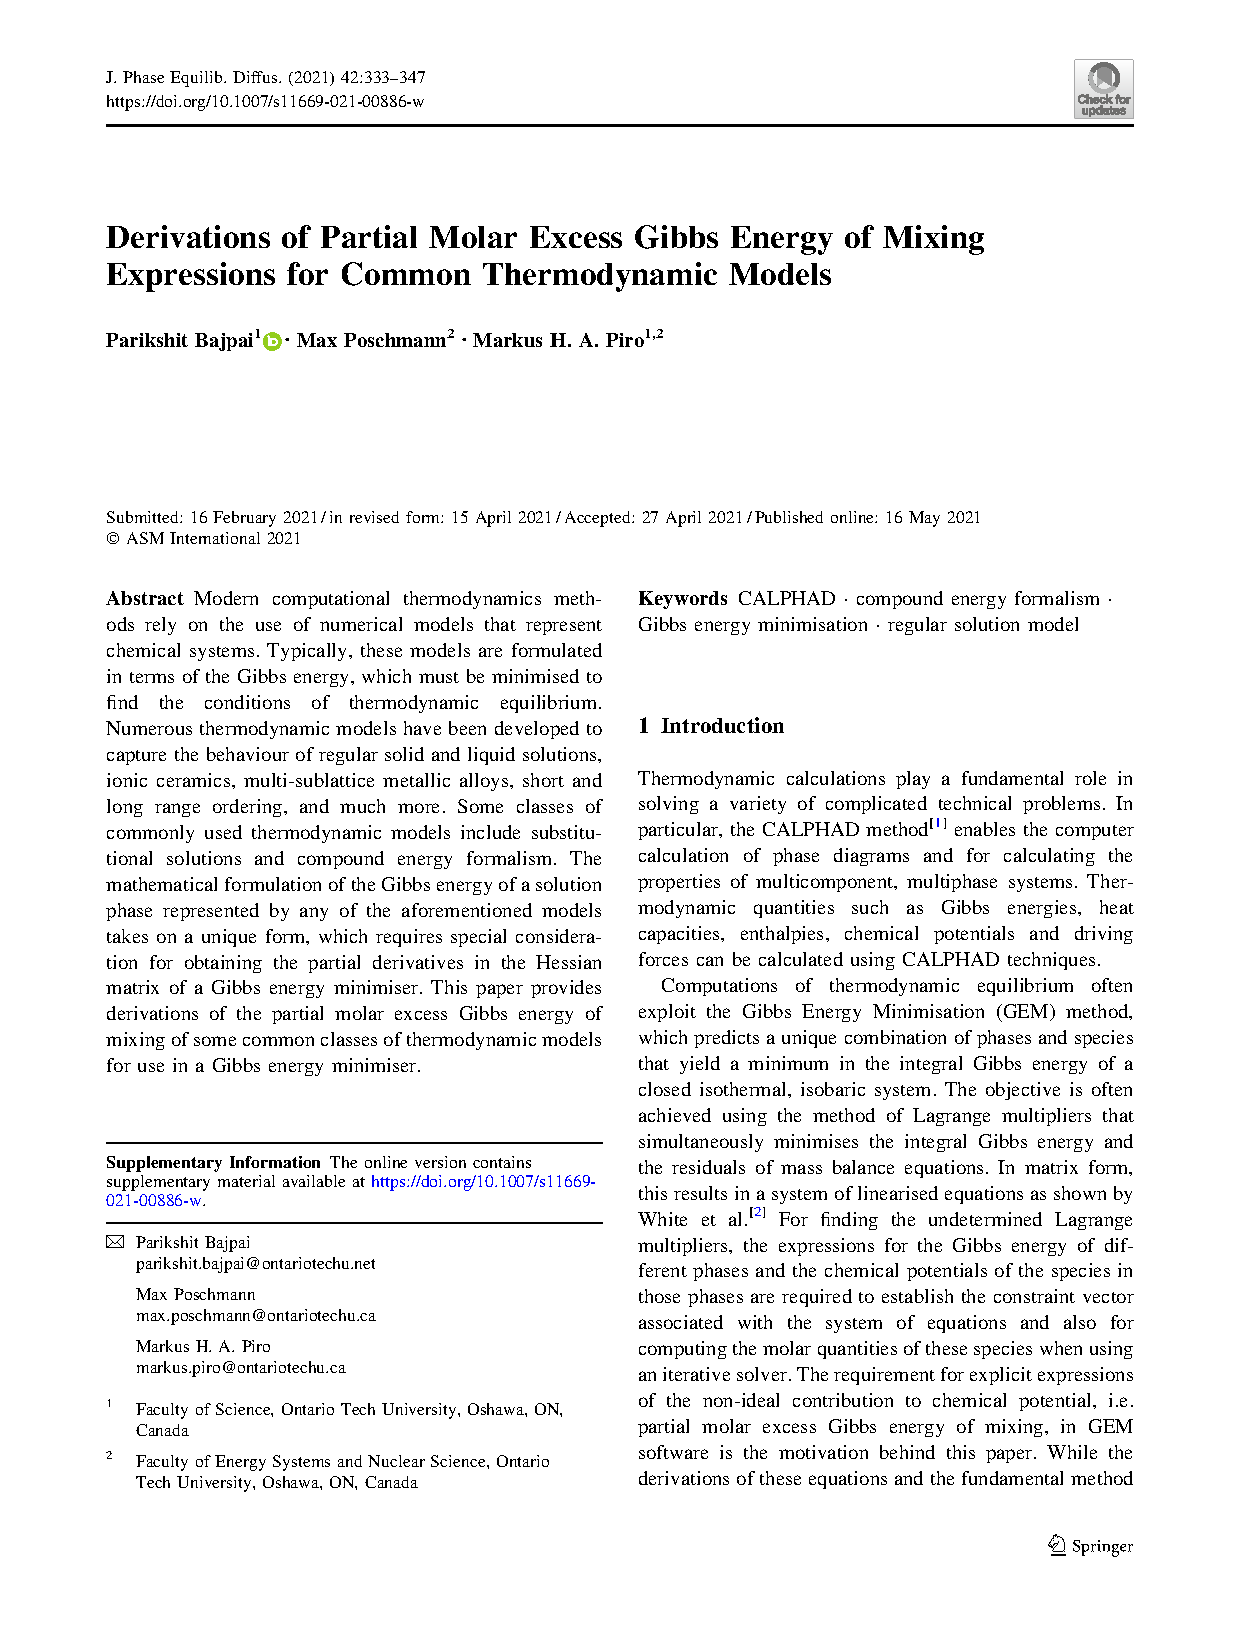
\includepdf[pages=-]{publications/Bajpai_2021_JPED.pdf}
	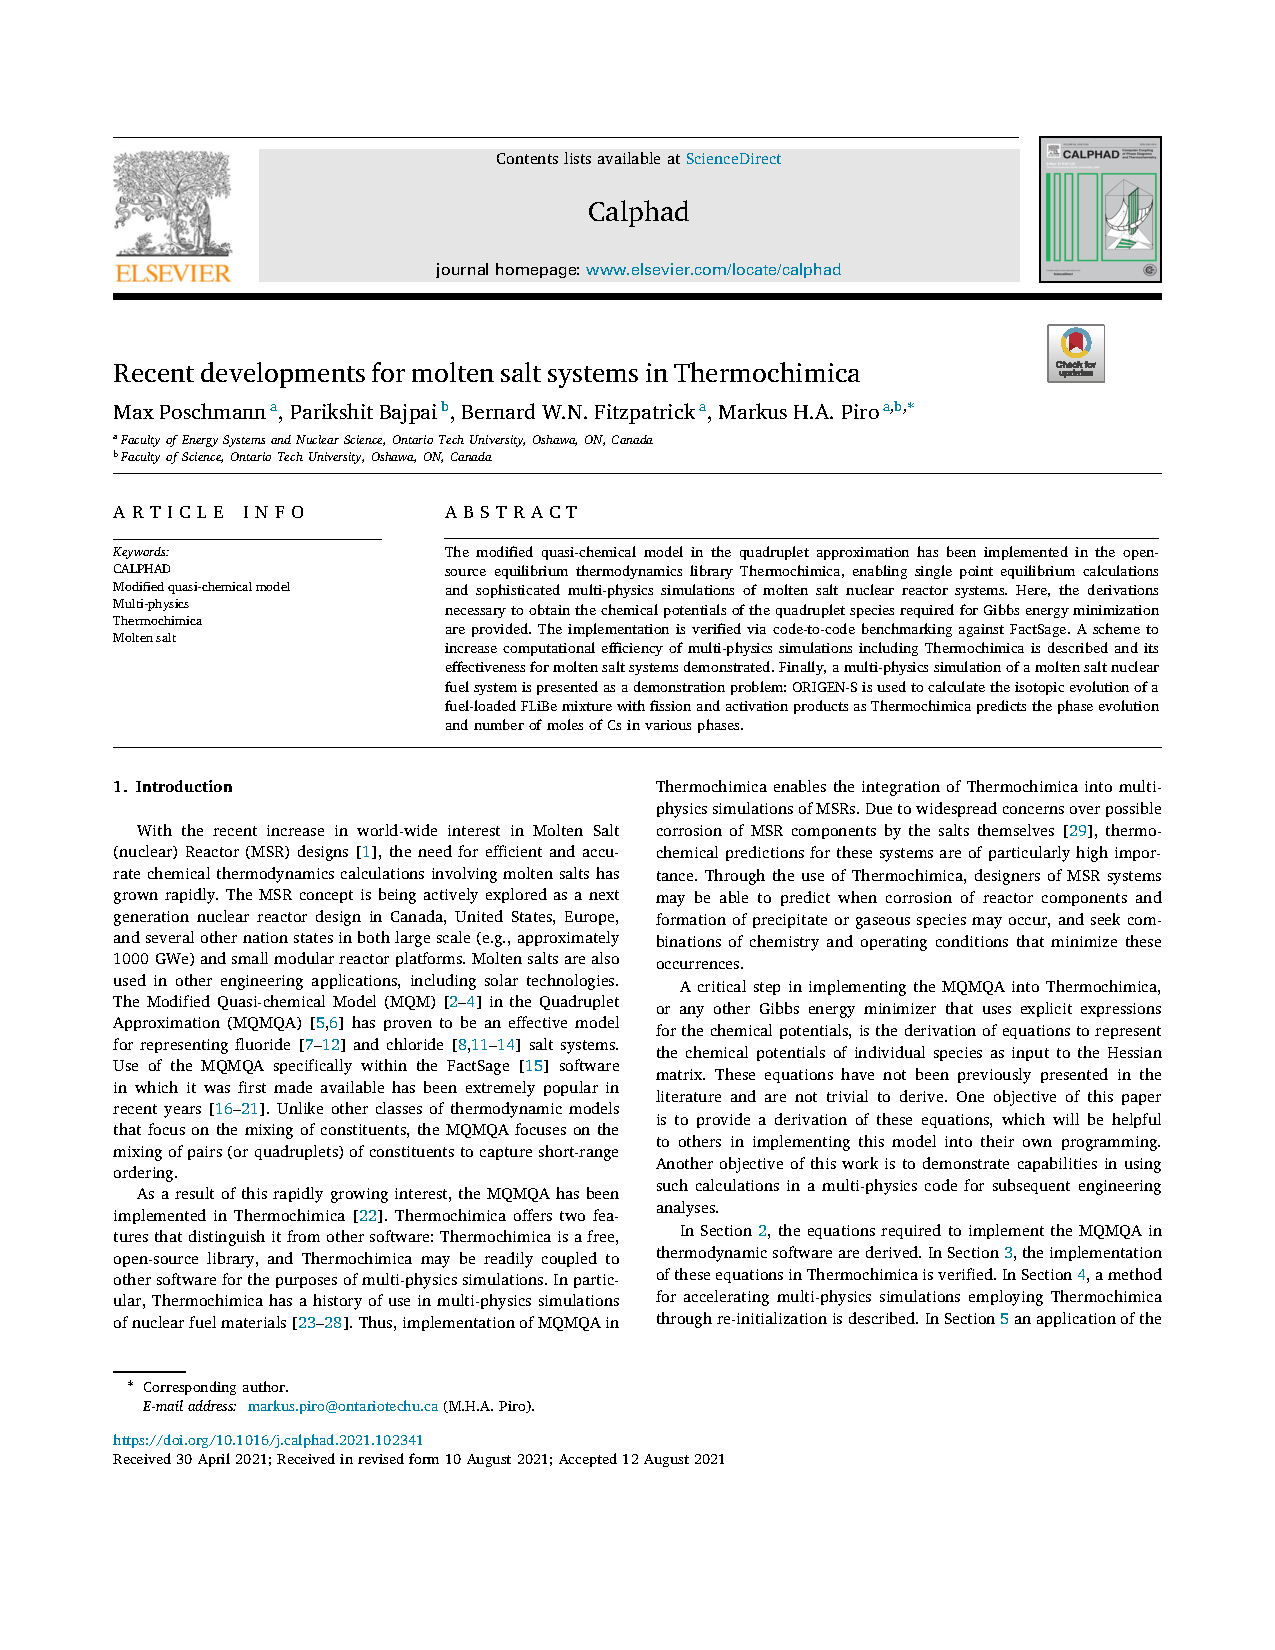
\includepdf[pages=-]{publications/Poschmann_2021_abridged.pdf}

\chapter{Equilibrium Thermodynamics} \label{chap:equilibrium}

	The foundations of thermodynamic equilibrium calculations were laid down by American chemical physicist Josiah Willard Gibbs who originally published his work \emph{On the Equilibrium of Heterogeneous Substances} in a relatively obscure American journal, the Transactions of the Connecticut Academy of Arts and Sciences, in several parts, during the years 1875 to 1878. Thermodynamic equilibrium computations in isothermal, isobaric systems are aimed at identifying a unique combination of phases and species which minimises the integral Gibbs energy of the system while satisfying the necessary underlying conditions. Thermodynamics requires that a favourable change in a system must decrease the Gibbs energy of the system while respecting the mass constraints of the system components and the Gibbs' phase rule must be satisfied.
	
%==============================================================================================================================
%													Phase Equilibrium
%==============================================================================================================================	
\section{Phase Equilibrium in Heterogeneous Systems} \label{sec:multi_eqb}
	A heterogeneous system is defined as one where the thermodynamic properties may have different values in different parts of the system when the system is at equilibrium. While a continuous variation of these properties is possible, equilibrium thermodynamics in the context of this work only concerns discontinuous variations where the properties have different values in different portions of the systems but are homogenous within each portion. A practical example of such a scenario is that of multiple phases being present in a system with the properties in phase being homogenous and the different phases are in equilibrium with each other \cite{liu_wang_2016}.
	
	In a system at equilibrium, with $C$ components, there are $C+2$ natural variables with $2$ representing the variables temperature, $T$, and pressure, $P$. For an isothermal, isobaric system, the equilibrium conditions result in:
	\begin{equation}
		d G_{\text{sys}} = -S dT -Vd(-P) + \sum_{i} \mu_j d n_j = 0.
	\end{equation}
	As a result, the equilibrium state is defined by a minimum in the integral Gibbs energy of the system at constant $T$, $P$ and $n_i$. In doing so one must respect the mass balance and charge neutrality constraints. In the present context, this also implies that the chemical potential of each component must be homogenous in all phases stable at equilibrium and gives the common tangent construction for phases at equilibrium:
	\begin{equation}
		\mu_{i}^{\phi_1} = \mu_{i}^{\phi_2} = \mu_{i}^{\phi_2} = \cdots,
	\end{equation}
	where $\phi_1$, $\phi_2$, etc. denote the phases stable at equilibrium. The above arguments can be generalised into the necessary and sufficient conditions for equilibrium which are used in the development of the Gibbs energy minimiser. 
%==============================================================================================================================
%													Conditions of Phase Equilibrium
%==============================================================================================================================

\section{Conditions of Phase Equilibrium} \label{sec:eqb_theory}
A thermodynamic equilibrium solver must meet both the necessary and sufficient conditions for thermodynamic equilibrium. Rooted in the fundamental laws of thermodynamics, the necessary and sufficient conditions together ensure that the Gibbs energy of the system is at a local equilibrium while respecting the constraints.

\subsection{Necessary conditions}
	The necessary conditions for thermodynamic equilibrium require satisfaction of mass conservation and the Gibbs' phase rule in addition to satisfying the Gibbs' criterion which is a generalisation of the common tangent construction. These condition can be summarised as follows.
	
	\begin{enumerate}
		\item \textbf{Conservation of mass}\\
			The law of conservation of mass requires that the linear equations representing mass constraints be satisfied. For component $j$, the mass balance equation can be written as:
			\begin{equation}\label{eq:massbalance}
				b_j = \sum_{\phi=1}^{\Phi} n_{\phi}\sum_{i=1}^{N_{\phi}} {\nu}_{ij} x_{i},
			\end{equation}
			where ${\nu}_{ij}$ represents the stoichiometric coefficient of element $j$ in phase species $i$. In an electrochemical system where the electrons form a system component with zero moles overall in the system, the mass balance constraint includes the charge neutrality constraint but it can be explicitly written as:
			\begin{equation}\label{eq:chargebalance}
				b_{e^-} = \sum_{i=1}^{N_{\phi}}x_{i}{\nu}_{i{e^-}} = 0.
			\end{equation} 
			
		\item \textbf{Gibbs' phase rule}\\
			Thermodynamic equilibrium conditions also require that the Gibbs' phase rule be satisfied. Gibbs' phase rule determines the \emph{degree of freedom} of the system, i.e., the number of phases that can be stable at equilibrium in relation to the state variables \cite{Gibbs:1878aa}. In general, the phase rule can be written as:
			\begin{equation}
                			F=C-\Phi + 2 + \Xi,
            		\end{equation}
            		where $F$ represents the degrees of freedom, $C$ denotes the number of components in the system, $\Phi$ denotes the number of phases and $\Xi$ denotes the number of ionic phases. However, for isothermal, isobaric systems with no charged species, the phase rule takes the following simplified form :
			\begin{equation}
                			F=C-\Phi,
            		\end{equation}
			which implies that the number of phases that can co-exist at equilibrium cannot exceed the number of components in a closed isothermal, isobaric system.
			
		\item \textbf{Gibbs' criterion}\\
			Ensuring that the Gibbs phase rule and mass balance constraints are satisfied is relatively straightforward but special attention must be paid to ensuring that the integral Gibbs energy of the system is at a minimum. The equilibrium criteria established by Gibbs requires that at equilibrium $d G_\text{sys} = 0$ \cite{Gibbs:1878aa}. Thus, differentiating equation~\eqref{eqn:integralGibbs}:
			\begin{equation}\label{eqn:dGibbs1}
				d G_{\text{sys}} = \sum_{\phi=1}^{\Phi} \sum_{i=1}^{N_{\phi}} \left( d n_{i}\mu_{i} + n_{i} d \mu_{i}\right) = 0.
			\end{equation}
			The chemical potentials are related through the \emph{Gibbs-Duhem equation} which, at constant temperature and pressure, can be written as \cite{Olander08}:
			\begin{equation}\label{eqn:dGibbs2}
				\sum_{\phi=1}^{\Phi} \sum_{i=1}^{N_{\phi}} \left( n_{i} d \mu_{i}\right) = 0.
			\end{equation}
			Substituting the Gibbs-Duhem equation in equation~\eqref{eqn:dGibbs2} gives:
			\begin{equation}\label{eqn:dGibbs3}
				d G_{\text{sys}} = \sum_{\phi=1}^{\Phi} \sum_{i=1}^{N_{\phi}} \left( d n_{i}\mu_{i} \right) = 0.
			\end{equation}
			The chemical potentials of the species can be written in terms of the chemical potentials of the system components. Therefore, substituting equation~\eqref{eq:massbalance} into equation~\eqref{eq:elempot}, differentiating with respect to $n_{i}$ at constant temperature and pressure and equating to zero gives:
			\begin{equation}\label{eqn:dGibbs4}
				d G_{\text{sys}} = \sum_{\phi=1}^{\Phi} \sum_{i=1}^{N_{\phi}}  d n_{i}\sum_{j=1}^{C}\nu_{ij}\Gamma_j  = 0,
			\end{equation}
			and rearranging the above results in:
			\begin{equation}\label{eqn:dGibbs5}
				\sum_{\phi=1}^{\Phi} \sum_{i=1}^{N_{\phi}}  d n_{i} \left( \mu_{i} - \sum_{j=1}^{C}\nu_{ij}\Gamma_j \right) = 0.
			\end{equation}
		Since both $\nu_{ij}$ and $\mu_{i}$ are unique for every species, the chemical potentials of species or phase in the system can be related to chemical potentials of system component at equilibrium through the following equation \cite{vanZeggeren11}:
		\begin{equation}\label{eq:Gibbs_criterion}
			\mu_{i(\phi)} = \sum_{j=1}^{C}\nu_{ij}\Gamma_j.
		\end{equation}
		Equation~\eqref{eq:mu_ex} is known as \emph{Gibbs' criterion} and ensuring that it is satisfied for all species in the system is equivalent to satisfying the equilibrium criterion that the Gibbs energy of the system be at a local minimum. This is useful in developing a convergence criterion for thermodynamic equilibrium calculations.
	\end{enumerate}	
	
\subsection{Sufficient conditions}
	The linear equality in equation~\eqref{eq:mu_ex} justifies the selection of stable species and making sure that no metastable species gets added to the system. However, satisfying the linear equation is insufficient to conclude that the system is at a \emph{global} minimum since $g_{\phi}^{ex}$ can be non-convex \cite{Piro16}. The driving force of a phase, $\Delta G_{\phi} $, is used to determine whether a system involving that phase is more stable than the previous system, which is defined as:
	\begin{equation}
        		\Delta G_{\phi}= \min_{\lambda} \sum_{i=1}^{N_{\lambda}}x_{i} \left (\mu_{i} - \sum_{j=1}^C \nu_{ij}\Gamma_j \right ),
    	\end{equation}
	which is subject to the following linear equality and inequality constraints:
	\begin{align}
		\sum_{i=1}^{N_\phi} x_i = 1, \; x_i > 0, \; \forall i \in \phi.
	\end{align}
	
%==============================================================================================================================
%												Methods for Calculating Phase Equilibrium
%==============================================================================================================================

\section{Computing Phase Equilibria}
Accurate and computationally efficient determination of equilibrium from the conditions mentioned in the previous section require careful consideration of the numerical method employed in the solver. Over the years, numerous strategies have been developed to solve the equilibrium thermodynamics problems but the two most relevant methods are the \emph{Gibbs Energy Minimisation} by White, Johnson and Dantzig \cite{White:58} which is based on the method of steepest descent of second order and the \emph{Partitioning of Free Energy}  which was also proposed by White \cite{White67} but is substantially different from Gibbs energy minimisation.

The goal of both Gibbs energy minimisation (GEM) and partitioning of Gibbs energy (PGE) approaches is to predict a unique combination of phases and species that minimise the integral Gibbs energy of an isothermal, isobaric system at a given composition. As in equation~\eqref{eqn:integralGibbs}, the integral Gibbs energy of a multicomponent multiphase system can be represented as:
\begin{equation}\label{eq:int_gibbs}
    G = RT \left(\sumsolnphase \molesol \sumspecies \molefrac{i} \cps{i} + \sumstoichphase \molestoich \cpst\right),
\end{equation}
where the symbols represent their usual variables mentioned before. 
As the conditions that must be satisfied at thermodynamic equilibrium have already been mentioned, the numerical procedures for  both the approaches can now be elaborated.

\subsection{Method of Lagrange multipliers}
White et al. \cite{White:58} established a second order steepest descent method for Gibbs energy minimisation which is based on the method of Lagrange multipliers for constrained optimisation. The GEM approach simultaneously optimises mass balance constraint and Gibbs' criterion while fixing the system size through the Gibbs phase rule. The dimensionless form of Gibbs energy of the system can be expressed as a quadratic approximation obtained by the Taylor series expansion as follows:
  \begin{equation}\label{eq:GibbsTaylor}
    \begin{split}
      \tilde{Q}^{m+1} = \tilde{G}^{m} &+ \left .\sumstoichphase \Delta_{\omega} \pder{\tilde{G}^m}{\molestoich^m} \right \vert_{\molestoich^m = \molestoich^{m+1}} \\
                      &+ \left . \sumsolnphase \sumspecies \Delta_i \pder{\tilde{G}^m}{\molespecies{i}^m}\right \vert_{\molespecies{i}^m = \molespecies{i}^{m+1}} \\
                      &+ \left . \frac{1}{2} \sumstoichphase \Delta^2_{\omega} \ppder{\tilde{G}^m}{\molestoich^m} \right \vert_{\molestoich^m = \molestoich^{m+1}} \\
                      &+ \left . \frac{1}{2} \sumsolnphase \sumspecies \sumspecies[l] \Delta_i \Delta_l \pqder{\tilde{G}^m}{\molespecies{i}^m}{\molespecies{l}^m} \right \vert_{\molespecies{i}^m = \molespecies{i}^{m+1}},
    \end{split}
  \end{equation}
where the superscript $m$ and $m+1$ denote the iteration at which the Gibbs energy is calculated and the deltas can be represented as follows:
  \begin{gather}
      \Delta_i = \molespecies{i}^{m+1} - \molespecies{i}^{m},\\
      \Delta_\lambda = \molesol^{m+1} - \molesol^{m}, \\
      \Delta_\omega = \molestoich^{m+1} - \molestoich^{m}.
  \end{gather}

While the first order partial derivatives are equal to the chemical potentials as shown in equation~\eqref{eq:mu_def}, the second order derivatives are as follows:
\begin{gather}
  \ppder{\tilde{G}^m}{\molestoich^m} = 0, \label{eq:partial1}\\
  \ppder{\tilde{G}^m}{\molespecies{i}^m} = \frac{1}{\molespecies{i}^m} - \frac{1}{\molesol^m}, \label{eq:partial2} \\
  \pqder{\tilde{G}^m}{\molespecies{i}^m}{\molespecies{l \neq i}^m} = - \frac{1}{\molesol^m}. \label{eq:partial3}
\end{gather}

Substituting equations \eqref{eq:mu_def}~and~\eqref{eq:partial1}--\eqref{eq:partial3} into the second order approximation of Gibbs energy given by equation~\eqref{eq:GibbsTaylor}, one gets the following objective function:
\begin{equation}
  \tilde{Q}^{m+1} = \tilde{G}^{m} + \sumstoichphase \cpst^m
                  + \sumsolnphase \sumspecies \Delta_i \cps{i}^m
                  + \frac{1}{2} \sumsolnphase \sumspecies \molespecies{i}^m \left(\frac{\Delta_i}{\molespecies{i}} - \frac{\Delta_\lambda}{\molesol^m} \right)^2,
\end{equation}
which must be minimised subject to the mass balance constraint. In order to solve the constrained optimisation problem, the method of Lagrange multipliers can be used and the resulting Lagrangian function is defined as:
  \begin{equation}\label{eq:GEM_Lagrangian}
      \mathcal{L} = \tilde{Q}^{m+1} - \sumelements \pi_{j}^{m+1} \left(\moleelem{j} - \moleelem{j}^m\right),
  \end{equation}
where $\pi_{j}$ denote the dimensionless undetermined Lagrange multipliers\footnote{While $\lambda$ is commonly used to denote Lagrange multipliers, $\pi$ is used here to avoid confusion with the solution phase index $\lambda$.}. The Gibbs energy of the system and the mass balance residuals can be simultaneously minimised by equating the gradient of the Lagrangian function to zero:
\begin{equation}
  \nabla \mathcal{L} = 0.
\end{equation}
The elements of the gradient vector are found by taking the partial derivatives of  equation~\eqref{eq:GEM_Lagrangian} with respect to the number of moles of species $\molespecies{i}$ and $\molestoich$:
\begin{gather}
  \pder{\mathcal{L}}{\molespecies{i}} = \cps{i} - \sumelements \stoich{i}{j} \pi_j^{m+1} + \left(\frac{\molespecies{i}^{m+1}}{\molespecies{i}^{m}} - \frac{\molesol^{m+1}}{\molesol^{m}} \right), \label{eq:pderL1}\\
  \pder{\mathcal{L}}{\molestoich} = \cpst - \sumelements \stoich{\omega}{j} \pi_{j}^{m+1},\\
  \pder{\mathcal{L}}{\pi_j} = \moleelem{j} - \moleelem{j}^m.
\end{gather}

By rearranging the preceeding equations and substituting the mass balance constraint, the following equation is obtained:
\begin{equation}
  \moleelem{j} = \sumsolnphase \sumspecies \left(-\cps{i}^m + \frac{\molesol^{m+1}}{\molesol^{m}} + \sumelements[k] \stoich{i}{k} \pi_k^{m+1} \right)\molespecies{i}^m \stoich{i}{j} + \sumstoichphase \molestoich^m\stoich{i}{j}.
\end{equation}
Upon rearranging, the commonly used form proposed by Eriksson and Ros\'{e}n \cite{Eriksson73} is obtained:
\begin{multline}\label{eq:Hess1}
  \sumelements \underbrace{\sumsolnphase \sumspecies \molespecies{i}\stoich{i}{j}\stoich{i}{k}}_{r_{jk}} \pi_j^{m+1} +
  \sumsolnphase \underbrace{\sumspecies\molespecies{i} \stoich{i}{j}}_{\phi_{j\lambda}^m} \underbrace{\left(\frac{\molesol^{m+1}}{\molesol^{m}} - 1\right)}_{\pi_\lambda^{m+1}} \\
  + \sumstoichphase \molestoich^{m+1} \stoich{\omega}{j} =
  \moleelem{j} + \sumsolnphase \sumspecies \left(\cps{i}^{m+1} -1 \right)\molespecies{i}^{m} \stoich{i}{j}.
\end{multline}

The chemical potentials of the species in solution phases can be related to system component potentials by the following:
\begin{equation}\label{eq:Hess2}
  \sumelements \pi_j^{m+1} \phi_{j \lambda}^m = \sumspecies \cps{i}^m \molespecies{i}^m,
\end{equation}
and the chemical potentials of stoichiometric phases constrain the system component potentials through the following relationship:
\begin{equation}\label{eq:Hess3}
  \cpst = \sumelements\stoich{\omega}{j}\pi_j^{m+1}.
\end{equation}

Together, equations \eqref{eq:Hess1}--\eqref{eq:Hess3} results in the following system of linear equations:
\begin{equation} \label{eq:HessianEqn}
  \Hessian \Unknown = \Constraint
\end{equation}
where the unknown vector $\Unknown \in \mathbb{R}^N$ and the vector of constraints $\Constraint \in \mathbb{R}^N$ with the number of unknowns $N = E + \Lambda + \Omega$. The two can be expanded as:
% \begin{gather}
%   \Unknown = \begin{bmatrix}
%                 \pi_{j=1}^{m+1} & \dots & \pi_{j=E}^{m+1} & \pi_{\lambda=1}^{m+1} & \dots & \pi_{\lambda=\Lambda}^{m+1} &  n_{\omega=1}^{m+1} & \dots & n_{\omega=\Omega}^{m+1}
%             \end{bmatrix}^T,
%   \Constraint = \begin{bmatrix}
%                   \moleelem{j=1} + \sumsolnphase \sumspecies \left(\cps{i}^m -1 \right)\molespecies{i}^m\stoich{i}{j=1} \\
%                   \vdots \\
%                   \moleelem{j=E} + \sumsolnphase \sumspecies \left(\cps{i}^m -1 \right)\molespecies{i}^m\stoich{i}{j=E} \\
%                   \sumspecies \tilde{\mu}_{i(\lambda = 1)}^m n_{i(\lambda = 1)}^m \\
%                   \vdots \\
%                   \sumspecies \tilde{\mu}_{i(\lambda = \Lambda)}^m n_{i(\lambda = \Lambda)}^m \\
%                   \tilde{\mu}_{\omega = 1} \\
%                   \vdots \\
%                   \tilde{\mu}_{\omega = \Omega}
%                 \end{bmatrix}.
% \end{gather}
\begin{equation}
  \Unknown = \begin{bmatrix}
                \pi_{j=1}^{m+1} \\ \vdots \\ \pi_{j=E}^{m+1} \\ \pi_{\lambda=1}^{m+1} \\ \vdots \\ \pi_{\lambda=\Lambda}^{m+1} \\  n_{\omega=1}^{m+1} \\ \vdots \\ n_{\omega=\Omega}^{m+1}
            \end{bmatrix},
  \Constraint = \begin{bmatrix}
                  \moleelem{j=1} + \sumsolnphase \sumspecies \left(\cps{i}^m -1 \right)\molespecies{i}^m\stoich{i}{j=1} \\
                  \vdots \\
                  \moleelem{j=E} + \sumsolnphase \sumspecies \left(\cps{i}^m -1 \right)\molespecies{i}^m\stoich{i}{j=E} \\
                  \sumspecies \tilde{\mu}_{i(\lambda = 1)}^m n_{i(\lambda = 1)}^m \\
                  \vdots \\
                  \sumspecies \tilde{\mu}_{i(\lambda = \Lambda)}^m n_{i(\lambda = \Lambda)}^m \\
                  \tilde{\mu}_{\omega = 1} \\
                  \vdots \\
                  \tilde{\mu}_{\omega = \Omega}
                \end{bmatrix}.
\end{equation}

The Hessian matrix, \Hessian, is given as follows:
\begin{equation}\label{eq:GEM_mat}
\Hessian =
    \begin{bmatrix}
      r_{11} & \dots & r_{1E} & \phi_{11} & \dots & \phi_{1\Lambda} & \nu_{11} & \dots & \nu_{1\Omega} \\
      \vdots & \ddots & \vdots & \vdots & \ddots & \vdots & \vdots & \ddots & \vdots \\
      r_{E1} & \dots & r_{EE} & \phi_{E1} & \dots & \phi_{E\Lambda} & \nu_{E1} & \dots & \nu_{E\Omega} \\
      \phi_{11} & \dots & \phi_{1E} & 0 & \dots & 0 & 0 & \dots & 0 \\
      \vdots & \ddots & \vdots & \vdots & \ddots & \vdots & \vdots & \ddots & \vdots \\
      \phi_{\Lambda1} & \dots & \phi_{\Lambda E} & 0 & \dots & 0 & 0 & \dots & 0 \\
      \nu_{11} & \dots & \nu_{1E} & 0 & \dots & 0 & 0 & \dots & 0 \\
      \vdots & \ddots & \vdots & \vdots & \ddots & \vdots & \vdots & \ddots & \vdots \\
      \nu_{\Omega 1} & \dots & \nu_{\Omega E} & 0 & \dots & 0 & 0 & \dots & 0 \\
    \end{bmatrix},
\end{equation}
where the terms $r_{jk}$ and $\phi_{j\lambda}$ are defined in equation~\eqref{eq:Hess1} and $\nu_{\omega j}$ represents the stoichiometric coefficient of system component $j$ in stoichiometric compound $\omega$.

While solving equation~\eqref{eq:HessianEqn} gives the mole numbers of stoichiometric phases directly, the mole numbers of the species of solution phases must be computed using the following rearranged form of equation~\eqref{eq:pderL1}:
\begin{equation}
  \molespecies{i}^{m+1} = \molespecies{i}^{m+1}\left(-\cps{i}^m + \frac{\molesol^{m+1}}{\molesol^{m} - \sumelements\stoich{i}{j} \pi_j^{m+1}}\right).
\end{equation}

\subsection{Partitioning of Gibbs energy}
PGE is based on finding the roots of the mass balance residual by expressing the mole fraction as a function of system component potentials. The expression for chemical potential of a species from equation~\eqref{eq:mu_ex} can be substituted into equation~\eqref{eq:Gibbs_criterion} and upon rearranging one gets:
    \begin{equation}
        \molefrac{i} = \exp{\left(-\pmgref{i} - \pmgex{i} +  \sumelements \stoich{i}{j} \cpe{j}\right)}.
    \end{equation}

Substituting the previous equation into the mass balance equation~\eqref{eq:massbalance}, one can formally relate the mass balance equations to the element potentials and results in the following:
    \begin{equation}
        \moleelem{k}^m = \sumsolnphase \molesol^m \sumspecies \stoich{i}{k} \exp{\left(-\pmgref{i} - \pmgex{i} +  \sumelements \stoich{i}{j} \cpe{j}^m\right)} + \sumstoichphase \molestoich^m \stoich{\omega}{k},
    \end{equation}
where the superscript $m$ denotes that the mass of element $k$ is the estimated mass at iteration $m$ and not the true total amount of the element in the system which will be denoted by \moleelem{k} without the iteration index. At convergence, the two will be equal and the sum of the mole fractions of the species \molefrac{i} will be equal to unity.

The PGE method surmises to partitioning the Gibbs energy of the system among elements by manipulating $\cpe{j}^m$ together with $\molesol^m$
and $\molestoich^m$ in order to reduce the residuals of the mass balance equations to zero. While doing this, one must ensure that the Gibbs criterion given by equation~\eqref{eq:Gibbs_criterion} is always satisfied. Mathematically this is equivalent to finding the roots of the system of non-linear equations of mass balance. The residual of mass balance $\Delta\moleelem{k}^m$ at iteration $m$ can be defined as:
    \begin{equation}\label{eq:residual_b}
        \Delta\moleelem{k}^m = \sumsolnphase \molesol^m \sumspecies \stoich{i}{k} \exp{\left(-\pmgref{i} - \pmgex{i} +  \sumelements \stoich{i}{j} \cpe{j}^m\right)} + \sumstoichphase \molestoich^m \stoich{\omega}{k} - \moleelem{k}.
    \end{equation}

The subsidiary condition satisfying the requirement for the sum of all mole fraction to be equal to unity results in the following residual for each phase $\lambda$:
    \begin{equation}\label{eq:residual_x}
        \Delta x_\lambda^m = x_\lambda^m - 1,
    \end{equation}
where $x_\lambda^m$ denotes the sum of mole fractions of all species of phase $\lambda$ at iteration $m$ (i.e. $x_\lambda^m = \sumspecies \molefrac{i}$).

Finally, the chemical potentials of the stoichiometric phases constrain the adjustments applied to the element potentials through the Gibbs criterion and results in the following residual equation:
    \begin{equation}\label{eq:residual_mu}
        \Delta\cpst = \sumelements[k] \stoich{\omega}{k} \cpe{k} - \pmgrefst.
    \end{equation}

Together, the residual equations~\eqref{eq:residual_b}--\eqref{eq:residual_mu} result in the following system of equation with the objective of finding roots \Unknown{} of the residual vector \Residual{}:
    \begin{equation}\label{eq:system}
        \Residual (\Unknown) = 0,
    \end{equation}
where $\Residual \in \mathbb{R}^N$, $\Unknown \in \mathbb{R}^N$ and $N$ is the number of non-linear equations and corresponding unknown variables ($N = E + \Lambda + \Omega$). The residual vector, \Residual, can be expanded as:
\begin{equation}\label{eq:resvec}
    \Residual(\Unknown) = \begin{bmatrix}
                                \Delta\moleelem{k=1}^m & \dots & \Delta\moleelem{k=E}^m & \Delta x_{\lambda=1}^m & \dots & \Delta x_{\lambda=\Lambda}^m &  \Delta\tilde{\mu}_{\omega=1} & \dots & \Delta\tilde{\mu}_{\omega=\Omega}
                          \end{bmatrix}^T,
\end{equation}
where superscript $T$ denotes the transpose. The unknown system variable vector takes the following form:
\begin{equation}\label{eq:unknwnvec}
    \Unknown = \begin{bmatrix}
                    \cpe{k=1}^m & \dots & \cpe{k=E}^m & n_{\lambda=1}^m & \dots &  n_{\lambda=\Lambda}^m & n_{\omega=1}^m & \dots &  n_{\omega=\Omega}^m
                \end{bmatrix}^T.
\end{equation}

The roots of equation~\eqref{eq:system} can be found using the Newton-Raphson method. Given $\Residual:\mathbb{R}^N \rightarrow \mathbb{R}^N$ continuously differentiable and starting with an initial estimate $\Unknown^0$, the Newton-Raphson method for a system of nonlinear equations requires solving the following at each iteration $m$ \cite{Dennis:1996aa}:
\begin{gather}
    \Jacobian(\Unknown^m) \Step^m = -\Residual(\Unknown^m),\\
    \Unknown^{m+1} = \Unknown^m + \alpha^m \Step^{m},
\end{gather}
where $\alpha^m$ is a scaling factor selected using an appropriate line search algorithm and $\Step^m$ is the Newton step representing the adjustment to the system variables and is given by:
\begin{equation}
    \Step^{m} = \begin{bmatrix}
                    d\cpe{k=1}^m & \dots & d\cpe{k=E}^m & d n_{\lambda=1}^m & \dots & d n_{\lambda=\Lambda}^m & d n_{\omega=1}^m & \dots &  d n_{\omega=\Omega}^m
                \end{bmatrix}^T.
\end{equation}

The Jacobian matrix\footnote{It must be noted the Jacobian matrix from the partitioning of Gibbs energy method is equivalent to the Hessian matrix resulting from the Gibbs energy minimisation approach.} is defined as:
\begin{equation}
\Jacobian =
    \begin{bmatrix}
     \spder{\moleelem{1}^m}{\cpe{1}^m} & \dots & \spder{\moleelem{1}^m}{\cpe{E}^m} & \spder{\moleelem{1}^m}{n_{\lambda=1}^m} & \dots & \spder{\moleelem{1}^m}{n_{\lambda=\Lambda}^m} & \spder{\moleelem{1}^m}{n_{\omega=1}^m} & \dots & \spder{\moleelem{1}^m}{n_{\omega=\Omega}^m} \\
    \vdots & \ddots & \vdots & \vdots & \ddots & \vdots & \vdots & \ddots & \vdots \\
    \spder{\moleelem{E}^m}{\cpe{1}^m} & \dots & \spder{\moleelem{E}^m}{\cpe{E}^m} & \spder{\moleelem{E}^m}{n_{\lambda=1}^m} & \dots & \spder{\moleelem{E}^m}{n_{\lambda=\Lambda}^m} & \spder{\moleelem{E}^m}{n_{\omega=1}^m} & \dots & \spder{\moleelem{E}^m}{n_{\omega=\Omega}^m} \\
    \spder{\moleelem{1}^m}{n_{\lambda=1}^m} & \dots & \spder{\moleelem{1}^m}{n_{\lambda=\Lambda}^m} & 0 & \dots & 0 & 0 & \dots & 0 \\
    \vdots & \ddots & \vdots & \vdots & \ddots & \vdots & \vdots & \ddots & \vdots \\
    \spder{\moleelem{E}^m}{n_{\lambda=1}^m} & \dots & \spder{\moleelem{E}^m}{n_{\lambda=\Lambda}^m} & 0 & \dots & 0 & 0 & \dots & 0 \\
    \spder{\moleelem{1}^m}{n_{\omega=1}^m} & \dots & \spder{\moleelem{E}^m}{n_{\omega=1}^m} & 0 & \dots & 0 & 0 & \dots & 0 \\
    \vdots & \ddots & \vdots & \vdots & \ddots & \vdots & \vdots & \ddots & \vdots \\
    \spder{\moleelem{1}^m}{n_{\omega=\Omega}^m} & \dots & \spder{\moleelem{E}^m}{n_{\omega=\Omega}^m} & 0 & \dots & 0 & 0 & \dots & 0
    \end{bmatrix}
\end{equation}
where, the partials derivatives are defined as follows:
\begin{gather}
    \pder{\moleelem{j}^m}{\cpe{k}^m} = \sumsolnphase \molesol^m \sumspecies \molefrac{i}^m \stoich{i}{j} \stoich{i}{k}\\
    \pder{\moleelem{j}^m}{n_{\lambda}^m} = \sumspecies \molefrac{i}^m \stoich{i}{j} \\
    \pder{\moleelem{j}^m}{n_{\omega}^m} = \stoich{\omega}{j}.
\end{gather}

At every iteration step, the direction vector is computed and the system is adjusted until the convergence criteria are achieved.


\subsection{Convergence criteria}
	A number of different methods can be proposed to judge the convergence of a thermodynamic equilibrium solver, the most obvious being ensuring that the relative change in Gibbs energy between two iterations is within a specified tolerance. Another approach that makes better use of principles of thermodynamic equilibrium is based on equation~\eqref{eq:mu_ex} and requires that the chemical potentials of all species lie on or above the Gibbs plane formed by chemical potentials of system components.
	\begin{enumerate}
		\item \textbf{Tolerance of} $G_\text{sys}^m$\\
		The most obvious method of ensuring convergence is to ensure that the normalised absolute difference of Gibbs energy, $\Psi_G$, between subsequent iterations is within a specified tolerance. Mathematically, this can be expressed as:
		\begin{equation}\label{eqn:conv1}
			\Psi_G = \left \vert \frac{G_\text{sys}^{m} - G_\text{sys}^{m-1}}{G_\text{sys}^{m}} \right \vert < \epsilon,
		\end{equation}
		where $\epsilon$ denotes the specified tolerance and the superscripts refer to iteration $m$ and $m-1$ respectively. Using the interpretation of Lagrange multipliers in the Gibbs Energy Minimisation (GEM) method proposed by White et al. \cite{White:58}, we can obtain a similar estimate of convergence. Since the Lagrange multipliers, $\pi_{j}$, denote the chemical potentials, they can be related to Gibbs energy of the system, $G_{sys}$. This can be mathematically expressed as:
		\begin{equation}\label{eqn:conv2}
			\Psi_{\pi} = \left \vert \frac{\pi_{j}^{m} - \pi_{j}^{m-1}}{\pi_{j}^{m}} \right \vert < \epsilon.
		\end{equation}
		Though intuitive, this approach to judging convergence suffers from two potential issues. The first issue is commonly observed in iterative solutions of non-linear systems where numerical stagnation can occur when significant numerical dampening is required to maintain the stability of numerical algorithm. In GEM for large chemical components, numerical dampening is often required and false convergence can result when the approach to minimum Gibbs energy becomes extremely slow.  The second issue relates to insignificant contribution to the Gibbs energy of the system  by minor species. These minor species can often be incorrect by several orders of magnitude and though they don't contribute to Gibbs energy significantly, they might be of significant chemical or radiological importance and the false sense of convergence can then lead to significant problems \cite{Piro11a}.

		\item \textbf{Gibbs' Criterion}\\
	 The Gibbs criteria for judging convergence relies on the relationship between chemical potentials and Gibbs energies. To utilise this concept, the chemical potentials can be expressed per gram-atom as:
	 \begin{equation}
	 	\hat{\mu}_{i} = \frac{{\mu}_i}{a_{i(T)}},
	 \end{equation}
	 where $\hat{\mu}_{i}$ [\si{\joule \per g-at}] is the chemical potential and ${a_{i(T)}}$  is the total number of atoms in the formula mass. This method of defining chemical potentials allows an equivalent comparison of chemical potentials of compounds with different numbers of atoms per molar mass.

	 At equilibrium, all $\hat{\mu}_{i}$ must lie on a hyper-plane at equilibrium in the $C$-dimensional Euclidean space, where $C$ represents the number of system components. This plane is called the \emph{Gibbs plane} and an example of it is shown in figure~\ref{fig:GibbsPlane} for a three dimensional space.
	 \begin{figure}[h!]
		\centering
		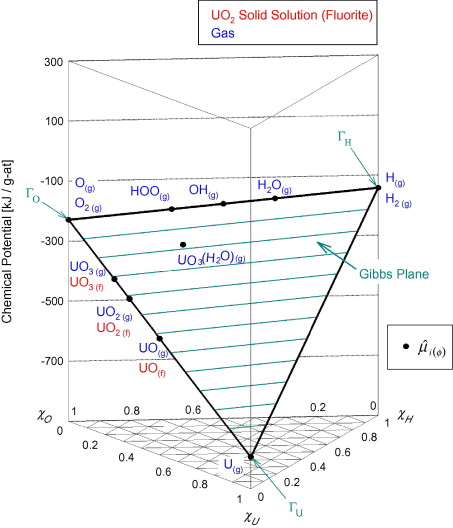
\includegraphics[width=0.6\textwidth]{figures/chapter-4/Gibbs_plane.jpg}
		\caption[The Gibbs criteria is satisfied when the chemical potentials for all species represented per gram-atom lie on the Gibbs Plane within an acceptable tolerance.]{The Gibbs criteria is satisfied when the chemical potentials for all species represented per gram-atom lie on the Gibbs Plane within an acceptable tolerance \cite{Piro11a}.}
		\label{fig:GibbsPlane}
	\end{figure}

	The chemical potential of any point on the Gibbs plane can be expressed as a linear combination of  chemical potentials of system components and this interpolated potential can be denoted by $\hat{\mu}_{i(\phi)}(\Gamma)$. The absolute difference between $\hat{\mu}_{i(\phi)}(\Gamma)$ and $\hat{\mu}_{i(\phi)}$, $\Psi_{\Gamma}$ can then be used as convergence criterion:
		\begin{equation}\label{eqn:convGC}
			\Psi_{\Gamma} = \left \vert  \hat{\mu}_{i(\phi)}(\Gamma) - \hat{\mu}_{i(\phi)} \right \vert < \epsilon,
		\end{equation}
	 i.e., all the species in equilibrium must lie on the Gibbs plane. If a phase lies below the Gibbs plane, adding it to the phase assemblage would yield a lower Gibbs energy of the system and such a system would not be at a global minimum. The Gibbs criteria is easily extendable to electrochemical equilibrium and can be conveniently implemented in a thermodynamic equilibrium solver \cite{Piro11a}.
	 \end{enumerate}
	 
\subsection{Choice of numerical algorithm}\label{sec:algo_choice}
	Both GEM and PGE have advantages and disadvantages and the choice of the algorithm must be based on the applications and excess mixing models used in them. For {\GEM}, the Gibbs energy minimisation method was selected and the reasoning behind it has been explained by Bajpai et al. \cite{Bajpai:2021ab}. While the paper, presented on the following pages, was written primarily for the thermochemistry library Thermochimica, the goal was also to pre-emptively justify the choice of the algorithm for {\GEM}. 
	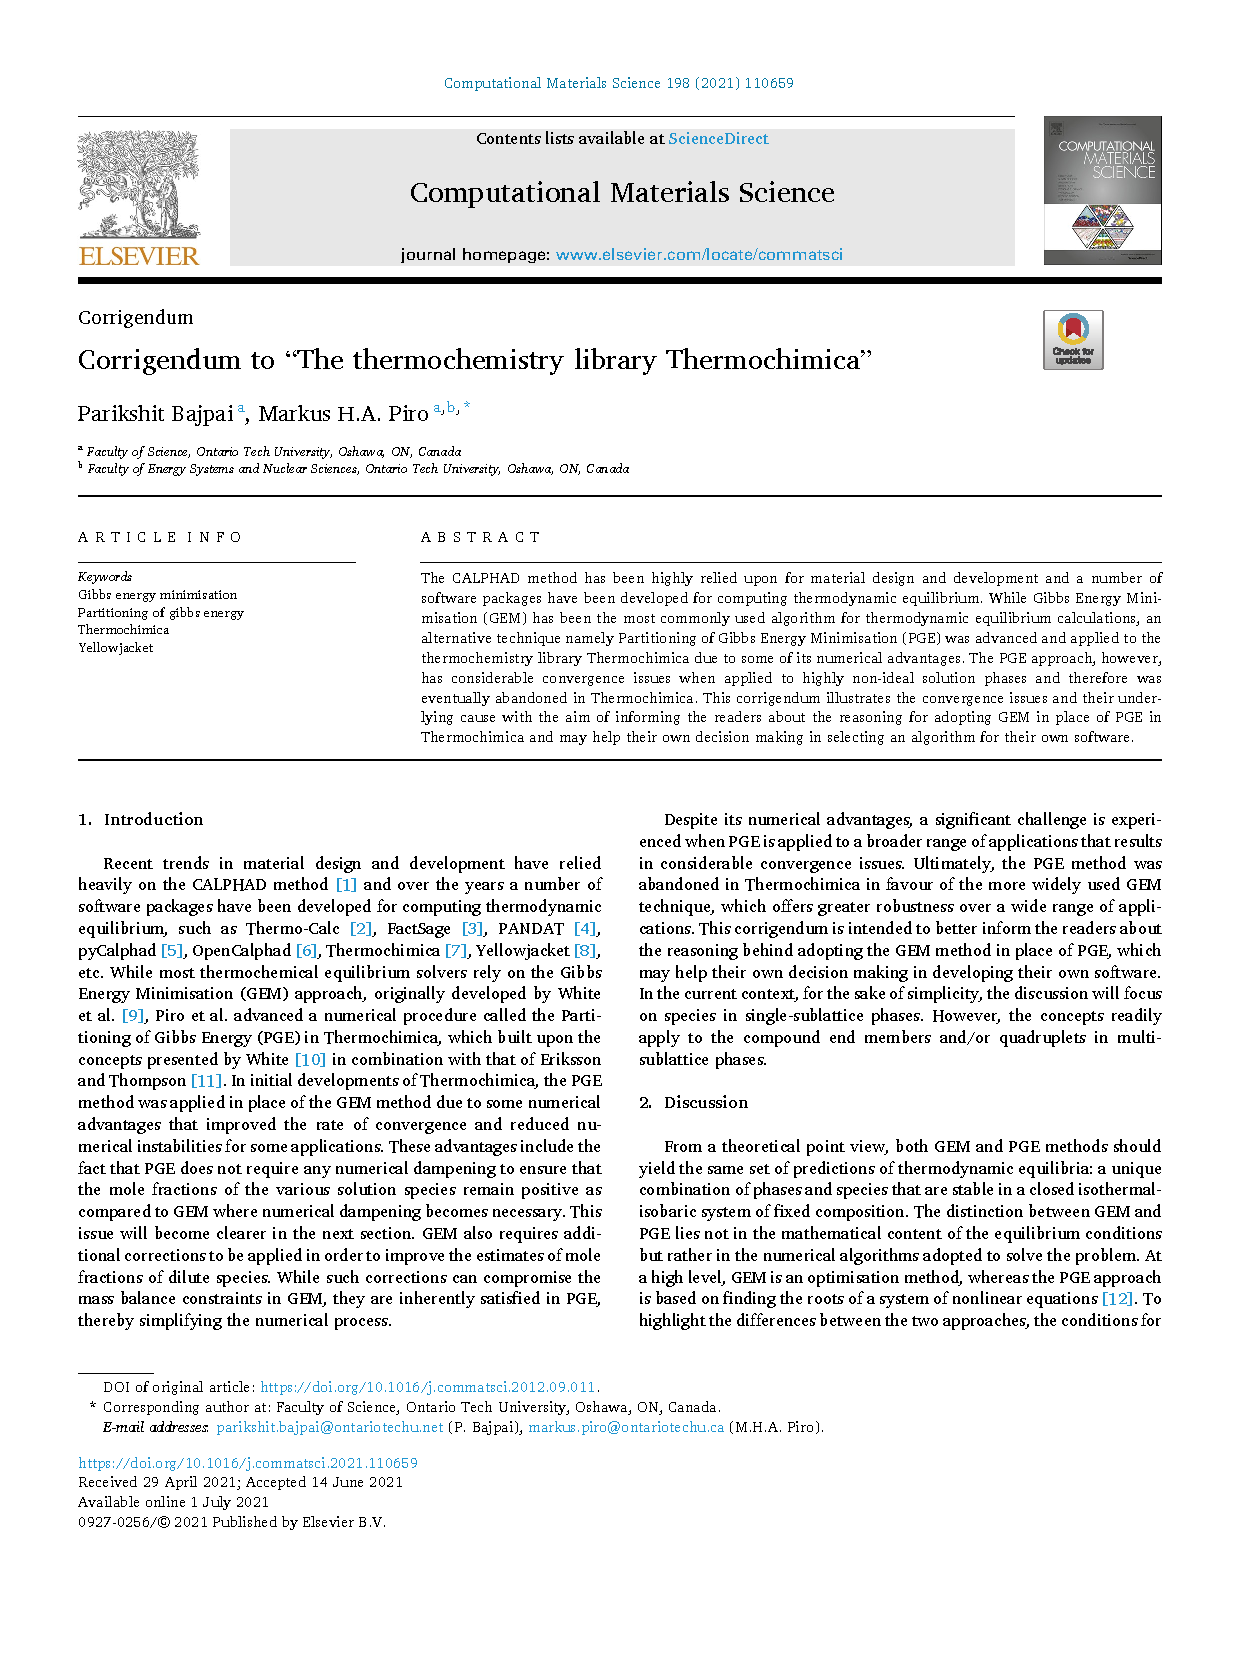
\includepdf[pages=-]{publications/Bajpai_2021_CMS.pdf}
	 
%==============================================================================================================================
%														Global Optimisation
%==============================================================================================================================

\section{Global Energy Minimisation}\label{sec:global_opt_intro}
	 Global minimisation of Gibbs energy is crucial to accurately predicting the stable phase assemblage using equilibrium thermodynamic softwares. An example application is the detection of miscibility gaps in phases containing regions of compositional instability. In a miscibility gap, the same phase can appear with different compositions and finding the global minimum from among the many local minima can be a daunting challenge. For multi-component systems, the topology of the energy surfaces tends to become quite complex particularly when there are multiple non-ideal phases in the system. This significantly complicates the interaction of the Gibbs energy surface with the Gibbs hyperplane and an inadequate numerical approach may lead to a false sense of thermodynamic equilibrium despite being far from the true equilibrium. To illustrate how an inadequate solver may yield a false equilibrium, the following scenarios can be considered:
	\begin{enumerate}
	\item In the fictive binary system shown in figure~\ref{fig:go_sys-AB}, a solution phase $\alpha$ and a stoichiometric phase \ce{A3B2} can possibly coexist. While the stoichiometric phase \ce{A3B2} and solution phase $\alpha$ are predicted to be stable, as represented by the dashed tangent line, they are in fact metastable and a miscibility gap would yield a lower value of the integral Gibbs energy of the system, $G_\text{sys}$.
		\begin{figure}[htbp]
			\centering
			\includegraphics[width=0.75\textwidth]{figures/chapter-4/System_AB.pdf}
			\caption[Fictive system with miscibility gap showing a possible false positive from thermodynamic equilibrium solver.]{Fictive system with miscibility gap showing a possible false positive from thermodynamic equilibrium solver (after Piro and Simunovic \cite{Piro16}).}
			\label{fig:go_sys-AB}
		\end{figure}

	\item In the fictive binary system shown in figure~\ref{fig:go_sys-CD} which can have three possible solution phases, the $\delta$ phase is believed to be metastable but one must confirm that the combination of $\beta$ and $\gamma$ is most stable or if a different combination is more stable. However, it can be seen that inserting the $\delta$ phase into the system and replacing one of the other two phases would yield a lower value of the integral Gibbs energy of the system, $G_\text{sys}$.
		\begin{figure}[htbp]
			\centering
			\includegraphics[width=0.75\textwidth]{figures/chapter-4/System_CD.pdf}
			\caption[Fictive system with three possible phases showing a false positive from thermodynamic equilibrium solver wherein a wrong phase is believed to be present at equilibrium.]{Fictive system with three possible phases showing a false positive from thermodynamic equilibrium solver wherein a wrong phase is believed to be present at equilibrium (after Piro and Simunovic \cite{Piro16}).}
			\label{fig:go_sys-CD}
		\end{figure}
	\end{enumerate}

As previously mentioned in section~\ref{sec:eqb_theory}, satisfying the necessary conditions, specifically the Gibbs' Criterion, is equivalent to finding a local minimum but one must demonstrate that the driving force, $\Delta G$, is non-negative for all phases to be metastable. Throughout the iterative process, the driving force for all the metastable phases should be calculated to determine if a particular phase needs to be added to the system. At this point, two similar but distinct approaches to the problem of identifying phases with negative driving force can be adopted. In the first approach, the goal is only to find out whether or not a phase has a negative driving force while in the second approach the goal is to determine the minimum value of the driving force subject to the equality and inequality constraints mentioned previously. While the first approach can be computationally cheaper, the second approach can provide additional information about the state of the system. For instance, when multiple phases have a negative driving force, the phase with the most negative driving force can be added to the system. 

Since the driving force function can be non-convex, finding the most negative driving force is essentially a constrained global optimisation problem. The domain space of  the problem is defined by the number of species in the solution phase and, because the mole fractions of the species must lie in $(0,1)$, the search space is box constrained. Using the sufficient conditions previously mentioned, the Lagrangian function of the driving force of solution phase $\phi$ can be defined as:
	\begin{equation}\label{eq:DrivingForceLagrangian}
		\mathcal{L}_\phi = \sum_{i=1}^{N_\phi} x_i \left(\tilde{\mu}_i - \sum_{j=1}^{C} \nu_{ij} \tilde{\Gamma}_j \right)
						 - \lambda_\phi \left( \sum_{i=1}^{N_\phi} x_i - 1 \right)
						 - \lambda_{e^-} \left( \sum_{i=1}^{N_\phi} \nu_{i {e^-}} x_i - 1 \right),
	\end{equation}
	where the first Lagrange multiplier, $\lambda_phi$, imposes the constraint on mole fractions and the second multiplier, $\lambda_{e^-}$, extends the constraints to handle ionic phases where the charge neutrality constraint must also be satisfied. The natural constraint on mole fractions implies $x_i \in (0, 1)$ and the  unknowns in the above expression, $x_i$, $\lambda_\phi$ and $\lambda_{e^-}$, must lie in $\mathbb{R}^{N_\phi + 2}$. For phases without any ionic components, the dimension of the above problem reduces by one.  The Lagrangian function has a minimum value when $\nabla \mathcal{L} = 0$. Differentiating $\mathcal{L}$ with respect to $x_i$:
	\begin{equation}
		\frac{\partial \mathcal{L}}{\partial x_i}	= \tilde{\mu}_i -  \sum_{j=1}^{C} \nu_{ij} \tilde{\Gamma}_j - \lambda_\phi,
	\end{equation}
	which shows that the undetermined Lagrange multiplier, $\lambda_\phi$, is the same as the driving force of the phase, $\Delta G_\phi$. Differentiating with respect to $\lambda_\phi$ yields:
	\begin{equation}
		\frac{\partial \mathcal{L}}{\partial \lambda_\phi}	= 1 - \sum_{i=1}^{N_\phi} x_i,
	\end{equation}
	and taking the derivative with respect to $\lambda_{e^-}$ results in:
	\begin{equation}
		\frac{\partial \mathcal{L}}{\partial \lambda_{e^-}}	= 1 - \sum_{i=1}^{N_\phi} \nu_{i {e^-}} x_i.
	\end{equation}
	The system of non-linear equations above can be solved using many different non-linear solution methods such as by taking the second order Taylor expansion of the Lagrangian function. The global optimisation algorithms used in {\GEM} will be discussed in further details in chapter~\ref{chap:implementation}.
%==============================================================================================================================
%															Summary
%==============================================================================================================================

\section{Summary}
Based on the fundamental laws of thermodynamics, achieving thermochemical equilibrium in a system requires satisfaction of several conditions which are as follows:
%	\subsection{Necessary conditions}
    	\begin{enumerate}\compresslist
        		\item \emph{Conservation of mass} requires that the mass of element $j$, $b_j$, must satisfy the following mass balance equation:
            	\begin{equation*}
                		b_j = \sum_{\lambda=1}^{\Lambda} n_{\lambda}\sum_{i=1}^{N_{\lambda}}x_{i({\lambda})}{\nu}_{ij} +  \sum_{\omega=1}^{\Omega} n_{\omega}{\nu}_{\omega},
            	\end{equation*}
            	where ${\nu}_{ij}$ and ${\nu}_{\omega}$ represent the stoichiometric coefficients of element $j$ in solution phase species $j$ and stoichiometric phase $\omega$ respectively.
        		\item \emph{Gibbs' phase rule} which defines the thermodynamic degrees of freedom of the system must also be     satisfied:
            	\begin{equation*}
                		F=C-\Phi + 2 + \Xi,
            	\end{equation*}
            	where $F$ represents the degrees of freedom, $C$ denotes the number of components in the system, $\Phi$ denotes the number of phases and $\Xi$ denotes the number of ionic phases.
        		\item \emph{Gibbs' criteria} for equilibrium requires that the Gibbs energy of a system be at a global equilibrium. In equivalent terms, the chemical potential for each system component must have the same value in all stable phases within the system \cite{HILLERT198131}, where the chemical potential of any constituent in a stable phase can be defined as a linear function of the element potentials, $\Gamma_j$, as:
            	\begin{equation*}
		        \mu_{i} = \sum_{j=1}^C \nu_{i,j} \Gamma_j.
            	\end{equation*}
    	\end{enumerate}

%	\subsection{Sufficient conditions}
    	The necessary conditions for thermodynamic equilibrium require that the chemical potentials of all stable solution phase species and stoichiometric phases abide by the above equality, which is equivalent to Gibbs energy of the system being at a local minimum, and that the conservation of mass and the Gibbs phase rule are satisfied. The sufficient condition requires that all the metastable phases abide by the following conditions
    	\begin{equation*}
        		\Delta G_{\phi} = \min_{x} \sum_{i=1}^{N_{\phi}}x_{i} \left (\mu_{i} - \sum_{j=1}^C \nu_{ij}\Gamma_j \right ),
    	\end{equation*}
    	i.e., there must exist a Gibbs' plane such that the element potentials lie on the plane and the chemical potentials of all the species lie on or above the plane and the mole fraction of the species must satisfy the following constraints
	\begin{equation*}
        		\begin{aligned}
            		\sum_{i=1}^{N_{\phi}}x_{i} = 1, \\
			x_{i} \geq 0 \;\; \forall i,
        		\end{aligned}
    	\end{equation*}
    	i.e., the sum of mole fraction of all the species in a phase $\phi$ must be unity and that the individual mole fractions must be greater than or equal to zero.

    	The aforementioned conditions are used in Gibbs energy minimisers to find a unique combination of phases that are stable in the system. In such solvers, one must also carefully consider the role of the numerical algorithm and the convergence criteria to be adopted as these choices can have a significant impact on both computational performance and robustness of the solver.

\chapter{Literature Review} \label{chap:litreview}
\begin{abstract}
    Robust and fast methods for computing chemical equilibrium in complex systems are widely used in materials and chemical industries. While industrial applications essentially require calculation tools capable of discriminating between stable and unstable phases and converging to nontrivial solutions, numerical equilibrium calculations have historically focused on representing dominant chemical reactions using the Law of Mass Action. It was only during and after World War {II} that numerical approaches amenable to computer programming were developed. Since then, there has been significant growth in the number of methods and softwares for solving the equilibrium thermodynamics problem. The intent of this chapter is to review the current state-of-the-art and identify not only the gaps that must be filled but also to recognise the promising avenue that can be leveraged in this work. The chapter starts by reviewing the numerical methods and codes that have been used for computing thermodynamic equilibrium in the past and follows it with a survey of global optimisation methods used in the field. Lastly, some efforts at coupling thermodynamic equilibrium to other codes has been examined.
\end{abstract}
	
\section{Numerical Methods for Thermodynamic Equilibrium}
	Up until the 1940s, chemical equilibria computations were based on two different methods. The first relied heavily on the assumption that only a few molecular species would be present in the final equilibrium and the law of mass action could be applied to these systems and the resulting system of non-linear equations was solvable using the relatively unsophisticated techniques of the time. The second method relied on a tedious trial-and-error approach with the user's intuition playing a significant role \cite{vanZeggeren11}. It was only during the Second World War that, fuelled by the development of rockets, research towards developing computational methods for chemical equilibrium gained momentum. This research was mainly driven by the fact that an accurate knowledge of chemical equilibrium of the propellants was a requirement for the design of rockets. However, all the methods developed at the time were based on the law of mass action and the procedure was not scalable to very large systems where it would be difficult to account for all the possible reactions.

	The first major breakthrough in computerising chemical equilibrium calculations was made after the Second World war. In 1946, Brinkley came up with a generalised scheme to approach equilibrium computation by giving an analytical criterion for the number of independent components in a multi-component system \cite{vanZeggeren11}. However, the most significant breakthrough in the calculation of thermodynamic equilibria was made at the RAND Corporation by White, Johnson and Dantzig  \cite{White:58}. Since then a few other methods have been proposed but none has found as much success as the method proposed by White et al. In fact, even the method proposed by White et al. has only undergone a few minor changes and more recent algorithm developments have focused on other complimentary routines, such as initialisation, describes later. This section reviews the major methods that have been proposed to compute thermodynamic equilibria.

	\subsection{Equilibrium constants}
	The earliest computational method for finding thermodynamic equilibrium relied on the equilibrium constants of individual reactions and were primarily applied to gas phase equilibria. The equilibrium constant, $K$, is defined as follows:
	\begin{equation}\label{eq:eqbconst}
		K = \frac{\prod^{N_p} x_{i,p}^{\nu_i}}{\prod^{N_r} x_{i,r}^{\nu_i}},
	\end{equation}
	where $x_{i,p}$ and $x_{i,r}$ denote the mole fractions of species $i$ in product and reactants respectively, $\nu_i$ denotes the stoichiometric coefficient of $i$, and, $N_p$ and $N_r$ denote the number of product and reactants, respectively.

	While equation~\eqref{eq:eqbconst} is easily applicable to single reactions, calculating the concentration of species in multiple simultaneous reactions each with a unique equilibrium constant is quite laborious. The first computational procedure for the calculation of the composition at chemical equilibrium of systems of many constituents was proposed by Brinkley \cite{Brinkley:1947aa} and is known as \emph{Brinkley's method}. Subsequently, a number of modifications were made to this method resulting in a number of other variant methods, such as the \emph{Brinkley-Krieger-White method} \cite{Krieger:1948aa}, the \emph{NASA method} \cite{Zeleznik:1968aa}, etc. The Brinkley-Krieger-White method, also known as the \emph{Brinkley-Newton-Raphson} method, is perhaps the most popular and, as is evident from the name, used the Newton-Raphson method to solve the system of non-linear equations \cite{vanZeggeren11}. The NASA method \cite{Zeleznik:1968aa} shares the same fundamentals as the Brinkley's method.

	Although Brinkley's method serves well for small systems suitable for hand calculations, it relies heavily on user intuition and prior knowledge of the reactions taking place. Furthermore, it neglects the effects of non-ideality and its derivatives due to mathematical difficulties \cite{Zeleznik:1968aa}. Eventually, owing to generalities and numerical superiority of the Gibbs Energy Minimisation (GEM) method, the Brinkley method fell out of favour among the scientific community.

	\subsection{Computing thermodynamic equilibria}
	The numerical technique of minimising the Gibbs energy of the system was originally proposed by White, Johnson and Dantzig \cite{White:58} and is based on the method of steepest descent of second order and was therefore referred to as the \emph{Second Order Steepest Descent Method}. This methodology, now commonly described as \emph{Gibbs energy minimisation}, has also been called as the \emph{RAND method} owing to the employer of the developers of the method.

	Gibbs energy minimisation is based on identifying a unique combination of species and phases that yield a minimum in the integral Gibbs of a closed isothermal isobaric system from amongst the many possible candidates. The selection of candidates is based on the first and second laws of thermodynamic and is subject to the conditions of thermochemical equilibrium -- satisfaction of the Gibbs phase rule, conservation of mass. Numerically, this amounts to systematically adjusting the Lagrangian multipliers -- some which represent the chemical potential of the system components -- to change the estimated amount of each species, making the Gibbs energy of the system progressively more negative.

	While the initial popularity of the GEM method was fuelled by its generality,  reduced dependence on user intuition and convenience of programmability \cite{Zeleznik:1968aa}, several other advantages have become more apparent as time progressed. Boynton advanced the method to include stoichiometric phases coexisting with solution phases \cite{Boynton:1960aa} and Eriksson \cite{Eriksson:1975aa} demonstrated the use of the method for non-ideal solutions and showed that when dealing with multiple solution phases, the numerics do not get significantly complicated. In fact, the number of simultaneous linear equations to be solved is equal to the number of system components and the number of phases estimated to be stable at equilibrium \cite{vanZeggeren11,Boynton:1960aa,Eriksson:1975aa,Eriksson73}.

	Over a period of time, a number of other techniques have been proposed for the thermochemical equilibrium problem. Most of them, however, have relied on the original GEM method \cite{White:58} as the fundamental approach with minor modifications to adapt to the nature of specific problem at hand. These modifications include accounting for charged species \cite{ERIKSSON1979375}, accounting for non-traditional effects such as surface tension \cite{KOUKKARI200618}, magnetic ordering \cite{Eriksson90} and Donnan effect \cite{PAJARRE200658}. Some of the more significant variations, such as the \emph{First Order Steepest Descent Method} proposed by Storey and van Zeggeren \cite{Storey:1964aa}, demonstrated poorer performance and lacked the ability to distinguish between local minima and maxima \cite{Storey:1964aa,vanZeggeren11}. Another variation relies on removing the mass balance constraint resulting in an unconstrained optimisation problem. This method, proposed by Lantagne et al. and based on a penalty function using the Broyden-Fletcher-Goldfarb-Shanno (BFGS), technique simultaneously minimises two objective functions - Gibbs energy of the system and the residual of the mass constraint vector \cite{LANTAGNE1988589,Nocedal06}. The method must also satisfy the linear inequality constraints related to mole numbers being non-negative. While the approach offers the advantage of solving fewer linear equations, the dual optimisation method is less numerically stable compared to single optimisation methods \cite{Nocedal06}.

	An impediment in numerically solving thermodynamic equilibria is the requirement of an initial estimate for the optimisation. Eriksson and Thompson \cite{Eriksson89} proposed a method called \emph{Levelling}, which is capable of closely estimating the dominant species and their quantities in the phase assemblage. The process requires a relatively small number of iterations and the number of iterations to reach convergence does not rapidly increase with the number of species in the system. These characteristics of levelling are well suited to large systems, such as nuclear materials. Another problem that arises when using GEM method is the negative mole fraction arising due to the evaluation of logarithmic term while computing the chemical potentials. White et al. proposed using a numerical dampening technique to avoid erroneous results. Finally, ensuring that the Gibbs energy of the system is at global minimum and not at one of the many local equilibria is a significant challenge that must be handled properly to ensure correct results. Despite the challenges, GEM has been shown to be the best available method for computing thermodynamic equilibrium and is the de-facto default solver in almost all the thermodynamic equilibrium codes. Piro and Simunovic \cite{Piro12a} proposed an enhancement to levelling, which they called \emph{Post-Levelling}, to further improve on the initial estimate. In addition to the reference Gibbs energy terms, post-levelling accounts for the ideal mixing terms as well but unlike the non-linear solver, it doesn't take into account non-linear mixing. Though the method showed decent performance gains, it was often sensitive to the thermodynamic system in consideration.

    Another problem that can significantly compromise the performance of thermodynamic equilibrium codes is the need to change the phase assemblage when a phase which may yield a lower Gibbs energy is identified. 
    One must make several decisions when doing this - can a phase be directly added without violating conditions of equilibrium? If not, does a phase need to be removed and which phase will result in the quickest convergence. There has been no discussion of algorithms for handling phase change except for Piro and Simunovic \cite{Piro12a} who proposed a strategy for managing these choices.  Together, many of these algorithms can have significant impact on the performance of thermodynamic equilibrium solvers and even the simplest strategies can sometimes lead to significant performance gains.

	\subsection{Partitioning of Gibbs energy (PGE)}
	The developer of Gibbs energy minimisation, W.B. White, proposed another numerical technique named \emph{Partitioning of Free Energy}  \cite{White67}, which is substantially different from the GEM method. In this method, the mass equations are differentiated with respect to Lagrange multipliers and though a number of numerical advantages were shown, the method was only applicable to homogeneous systems comprised of ideal gas and could not be used for heterogeneous systems involving pure stoichiometric phases and/or multiple solution phases \cite{White67,vanZeggeren11}. The significant disadvantages of this method compared to GEM led to it being mostly dismissed by the thermodynamic community until Piro \cite{Piro11b} reconsidered a modified form of the method by incorporating principles of the levelling method and employed it in an earlier version  of thermochemistry library {Thermochimica} \cite{Piro13}.

	Piro's approach \cite{Piro13} constrains  Gibbs' phase rule  while iterating to satisfy the mass balance constraint. The method constrains the chemical potential of all species and phases in terms of the chemical potentials of the system components, thus formally relating the mass balance equations to the chemical potentials of the system components. The objective of the method is to partition the Gibbs energy of the system among the elements to minimise the residuals of the mass balances. Thus, in this method, the solver attempts to find the roots of the mass balance residual vector while the Gibbs criteria is inherently verified and need not be verified at every iteration thus simplifying the numerical approach. This approach can then be used for heterogeneous systems, which may include stoichiometric phases, ideal solution phases and even non-ideal solution phases.

	Numerically, GEM is an optimisation procedure while PGE solves for the roots of a simultaneous system of linear equation \cite{vanZeggeren11}. As a result, the chemical potential terms for the solution phase are included in the GEM method but absent from the functional vectors in PGE. Additionally, the approaches differ in the computation of a new set of mole numbers, which must be positive. Computation of non-negative logarithmic terms can result in non-real numbers in GEM causing numerical difficulties and necessitating the use of numerical dampening which in turn reduces the rate of convergence. However, in PGE, additional dampening is not required since the mole fractions, being defined as exponentials of real numbers, will always be positive.

	A disadvantage of the PGE method is that it requires moles fractions to be explicitly expressed as functions of chemical potentials of the species. As shown before, chemical potentials of the species can be uniquely expressed as a functions of mole fraction but not the other way around. Thus for non-ideal species, the PGE method fails in the absence of explicit functions of mole fractions in terms of chemical potentials. Despite all its numerical advantages, the PGE method proved to be less robust than the GEM approach and was eventually replaced by GEM in Thermochimica \cite{Bajpai:2021ab}. Though promising, the method has only been used in a limited number of other applications, a couple of them being by Riel et al. \cite{Riel:2022aa} and by Kruskopf \cite{Kruskopf:2018aa}.

	\subsection{Other methods}
	Several other numerical methods have been proposed for computing thermodynamic equilibria but none has received success like GEM. The most notable of these is the approach by Srinivas and Rangaiah which uses  the Random Tunnelling Algorithm (RTA) based on the concept of Terminal Repeller and Unconstrained Subenergy Tunnelling (TRUST) algorithm \cite{Srinivas06}. The TRUST algorithm is akin to the steepest descent method but differs in that the minimisation is performed in two stages - a local minimisation followed by global minimisation through tunnelling \cite{Nocedal06}.  However, the method is limited by the system size and shows satisfactory performance for relatively small systems of up to 10 variable \cite{Nocedal06}.

	Another method that was proposed by the developers of the GEM method is based on linear programming. George B. Dantzig applied the Simplex method to thermodynamic equilibrium problem at constant temperature and pressure \cite{Dantzig:1957aa,Dantzig:1958aa}. In the simplex method, a linear approximation of Gibbs energy of the system is minimised instead of the non-linear system. The linearised model is obtained by representing the logarithmic function in the chemical potential term by the following:
	\begin{equation}
		\beta_i = \alpha_i \ln \alpha_i
	\end{equation}
 which is represented as a piecewise linear approximation as shown in fig.~\ref{fig:simplex}.
 	\begin{figure}[htbp]
		\centering
		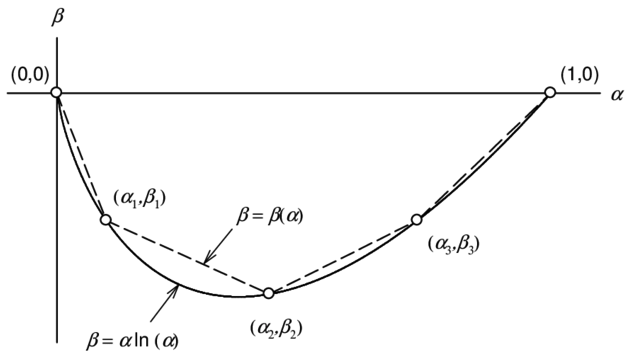
\includegraphics[width=0.75\textwidth]{figures/chapter-5/Simplex}
		\caption[Approximation of the function $\beta$ in simplex method.]{Approximation of the function $\beta$ in Simplex method. Reproduced by Piro \cite{Piro11b} from Dantzig et al. \cite{Dantzig:1957aa}}
		\label{fig:simplex}
	\end{figure}
	Though the Simplex method has been successful in many optimisation problems \cite{Dantzig:2016aa}, the linearisation of $\beta$ generates a relatively large number of additional unknowns and the computational expense becomes quite large. Furthermore, the method is unable to determine the composition of dilute species \cite{vanZeggeren11}. As a result, the simplex method has not received widespread usage in thermodynamic equilibrium calculations.


\subsection{Gibbs energy minimisers (GEM)}
	Over the years, a number of codes have been developed to compute thermodynamic equilibria in complex systems and many of these codes are summarised in Table~\ref{tab:gemreview}. The most noticeable of these codes include SOLGAS \cite{Eriksson71} and its successor SOLGASMIX \cite{Eriksson:1975aa}, which are well known for their versatility, computational efficiency and the widespread availability of source code. Moreover,  SOLGAS has been used as the solver in codes like HSC \cite{HSCSoftware:aa}, ChemSage \cite{Eriksson90} and FACT \cite{Thompson83}. FACT combined the thermodynamic equilibrium solver with a comprehensive thermodynamic database and, by implementing the levelling method, eliminated the need for the user to manually input initial estimates. This made FACT a popular choice in the thermodynamics community. FACT merged with ChemSage to create a new standalone software called FactSage \cite{Bale02}, which is the current version of the SOLGAS family. Another app in the family, called ChemApp \cite{Eriksson:2008aa,Petersen:2007aa}, is a software library that can be called from external codes and has similar capabilities as FactSage.

	Another family of popular thermodynamic equilibria tools is ThermoCalc \cite{ANDERSSON2002273} and is widely used in thermodynamic model development, thermodynamic equilibrium calculations, and  phase diagram construction. It has been developed for complex heterogeneous interaction systems with strongly non-ideal solution phases and can be applied to any thermodynamic system in the fields of chemistry, metallurgy, material science, alloy development, geochemistry, semiconductors etc. depending on the kind of database it is connected to. A unique advantage of ThermoCalc compared to other thermodynamic codes is that it allows explicit conditions on individual phase compositions or configuration whereas most software can handle conditions on the overall composition only. For example, activities and chemical potentials of the components, volumes, enthalpies, entropies etc can also be set as conditions.  OpenCalphad \cite{Sundman:2015aa} is an open-source code led by Bo Sundmann, one of the original developers of ThermoCalc, and it aims to provide facilities for multicomponent equilibrium calculations using the Compound Energy Formalism (CEF) and other models both for interactive calculations and in application software. It has been designed to allow interested scientists to develop thermodynamic models and assess model parameters for thermodynamic databases to describe experimental data as well as theoretical results from DFT calculations to calculate phase equilibria and phase diagrams. Another notable code developed with the goal of enabling uncertainty quantification is PyCalphad developed by Otis et al. \cite{Otis:2017aa}.

	Amongst the many thermodynamic equilibrium codes available in the open literature, one of the common limitations pertains to the relatively small number of standalone calculations that these codes are designed to perform. While suitable for problem specific calculations, where a few failures in convergence would have no significant bearing on the performance, these codes cannot be integrated into multiphysics softwares. In addition, since the mathematical difficulty in achieving convergence increases with the number of phases that can coexist in the system, most of these softwares  limit the maximum number of phases and system components that can be simultaneously considered. While this has no bearing on applications such as combustion, the limited number of phases that can be solved creates a severe impediment for nuclear applications.

	In the nuclear materials community, three code families have garnered particular attention - GEMINI \cite{Cheynet09}, ThermoCalc \cite{ANDERSSON2002273} and FactSage \cite{Bale02}. Due to their established reputation in the nuclear community, these codes have traditionally been applied in development of several thermodynamic treatments for nuclear fuels and materials. In fact these three codes offer a number of advantages over the other codes reviewed here, including the capability of handling a very large number of system components, phases and species, and the ability to use a wide range of sophisticated thermodynamic models.

    Table~\ref{tab:gemreview} summarises the current thermodynamic equilibrium codes which are available in open literature. The table classifies codes based on the choice of algorithms and the class of thermodynamic models that they support. While not explicitly written out in the table, most of the codes are only designed for handling small systems and aimed at creating phase diagrams. Of more interest to this work is the MQMQA model since it is the model most commonly used to describe molten salts. In fact, apart from commercial code FactSage in which the model was initially implemented, most codes did not support MQMQA until very recently. Recently, however, and in conjunction with the work done in this thesis, this model has been implemented in Thermochimica \cite{Poschmann:2021ab}. Lastly, only very recently, the model has been implemented in PyCalphad \cite{Palma:2022aa}. Even beyond MQMQA, most papers in the open literature don’t give sufficient details about models for one to easily adopt them into their own programming.
	
{%\newgeometry{margin=1cm}
%%\begin{landscape}
%\pagestyle{empty}
%		\begin{longtable}{p{0.15\textwidth} p{0.25\textwidth} p{0.1\textwidth} p{0.125\textwidth} p{0.125\textwidth} p{0.125\textwidth} p{0.125\textwidth}}
\renewcommand{\arraystretch}{0.7}
	\begin{longtable}{@{}lclcrcrcrcr@{}}
		\caption{A review of the major thermodynamic equilibrium codes.}\\
		\toprule
		\multicolumn{1}{c}{\multirow{2}{*}{\textbf{Code / Author}}} &\phantom{} & \multicolumn{1}{c}{\multirow{2}{*}{\textbf{Method}}} &\phantom{} & \multicolumn{7}{c}{\textbf{Models}} \\
		\cmidrule{5-11}
		\multicolumn{1}{c}{} & \phantom{} & \multicolumn{1}{c}{} & \phantom{} & \multicolumn{1}{c}{\textbf{Stoich.}} & \phantom{} & \multicolumn{1}{c}{\textbf{Ideal}} & \phantom{} & \multicolumn{1}{c}{\textbf{Non-ideal}} & \phantom{} & \multicolumn{1}{c}{\textbf{Ionic}} \\
		\midrule
		\endfirsthead
		\caption[]{A review of the major thermodynamic equilibrium codes (contd).}\\
		\toprule
		\multicolumn{1}{c}{\multirow{2}{*}{\textbf{Code / Author}}} &\phantom{} & \multicolumn{1}{c}{\multirow{2}{*}{\textbf{Method}}} &\phantom{} & \multicolumn{7}{c}{\textbf{Models}} \\
		\cmidrule{5-11}
		\multicolumn{1}{c}{} & \phantom{} & \multicolumn{1}{c}{} & \phantom{} & \multicolumn{1}{c}{\textbf{Stoich.}} & \phantom{} & \multicolumn{1}{c}{\textbf{Ideal}} & \phantom{} & \multicolumn{1}{c}{\textbf{Non-ideal}} & \phantom{} & \multicolumn{1}{c}{\textbf{Ionic}} \\
		\midrule
		\endhead
		ANGE (SAGE) \cite{Baurens:2014aa} && GEM && Yes && Yes && Yes && Yes \\
		CALMIX \cite{GREINER1988529} && GEM && Yes && Yes && Yes && No \\
		Cantera \cite{Goodwin:aa} && GEM && No && Yes && Yes && No \\
		Castier et al. \cite{CASTIER1989237} && GEM && No && Yes && No && No \\
		CatCalc \cite{Shobu09} &&GEM && Yes && Yes && Yes && No \\
		CEA \cite{Gordon94} && GEM && Yes && Yes && No && No \\
		ChemApp \cite{Eriksson:2008aa} && GEM && Yes && Yes && Yes && Yes\\
		ChemSage \cite{Eriksson90} && GEM && Yes && Yes && Yes && Yes\\
		ChemSheet \cite{Koukkari:2005aa} && GEM && Yes && Yes && Yes && Yes\\
		COEXIST \cite{Ahafat:1992aa} && Levelling && Yes && No && No && No\\
		Dantzig et al. \cite{Dantzig:1958aa}&& Simplex && No && Yes && No && No\\
		Ebel et al. \cite{Ebel:2000aa} && BNR && Yes && Yes && No && No\\
		ESP \cite{Rafal:2003aa} && LMA && No && Yes && No && No\\
		FACT \cite{Thompson83} && GEM && Yes && Yes && Yes && Yes\\
		FactSage \cite{Bale83} && GEM && Yes && Yes && Yes && Yes\\
		GEMINI 1 \cite{Cheynet09} && GEM && Yes && Yes && No && No\\
		GEMINI 2 \cite{Cheynet09} && GEM && Yes && Yes && Yes && Yes\\
		GEM-Selektor \cite{Karpov:aa} && GEM && Yes && Yes && No && Yes\\
		GEMIPM2K \cite{Karpov:aa} && GEM && Yes && Yes && No && Yes\\
		Gibbs \cite{COOL2010393} && C-Hull && {} && Yes && Yes && {}\\
		GLOPEQ \cite{MCDONALD19971} && GEM* && No && Yes && No && No\\
		HALTA \cite{Sillen:1962aa} && LMA && No && Yes && No && No\\
		HALTAFALL \cite{INGRI19671261} && LMA && Yes && Yes && No && No\\
		Han et al. \cite{HAN1998897} && LMA* && No && Yes && No && No\\
		HSC \cite{HSCSoftware:aa} && GEM && Yes && Yes && Yes && Yes\\
		Koukkari et al. \cite{KOUKKARI200618} && Const. GEM && Yes && Yes && Yes && Yes\\
		Kruskopf \cite{Kruskopf:2018aa} && PGE && Yes && Yes && Yes && Yes\\
		Lantagne et al. \cite{LANTAGNE1988589} && {GEM} && No && Yes && Yes && No\\
		Lee et al. \cite{PENGLEE19991183} && {GEM} && No && Yes && Yes && No\\
		Lukas et al. \cite{Lukas77} && {GEM} && Yes && Yes && Yes && No\\
		MAGEMin \cite{Riel:2022aa} && {PGE} &&  && Yes && Yes && \\
		MatCalc \cite{Kozeschnik:2001aa} && {GEM} &&  && Yes && Yes && \\
		MTDATA  \cite{Davies02} && {GEM} && No && Yes && Yes && No\\
		NUTS \cite{Loukusa:2014aa} && {GEM} && Yes && Yes && Yes && Yes\\
		OpenCalphad \cite{Sundman:2015aa} && {GEM} && Yes && Yes && Yes && Yes\\
		PANDAT \cite{Cao09} && {GEM} && Yes && Yes && Yes && Yes\\
		Pereira et al. \cite{PEREIRA20101} && {HEM} && No && Yes && No && No\\
		PyCalphad \cite{Otis:2017aa} && {Lower C-Hull} && Yes && Yes && Yes && No\\
		Rossi et al. \cite{ROSSI20111226} && GEM && Yes && Yes && No && No\\
		Schnedler \cite{SCHNEDLER1984265} && GEM && Yes && Yes && No && No\\
		Smith and Missen \cite{Smith:1988aa} && GEM && No && Yes && No && No\\
		SOLGAS \cite{Eriksson71} && GEM && No && Yes && No && No\\
		SOLGASMIX \cite{Eriksson:1975aa} && GEM && Yes && Yes && Yes && No\\
		SOLGASMIX-PV \cite{Besmann:1977aa} && GEM && Yes && Yes && Yes && No\\
		SOLGASWATER \cite{ERIKSSON1979375} && GEM && Yes && Yes && Yes && Yes\\
		Song et al. \cite{SONG19912513} && GEM* && Yes && Yes && No && No\\
		Srinivas et al. \cite{Srinivas06} && GEM-RTA && No && Yes && No && No\\
		STANJAN / EQUIL \cite{Reynolds86} && PGE && No && Yes && No && No\\
		Storey et al. \cite{Storey:1964aa} && GEM && Yes && Yes && No && No\\
		THERIAK \cite{DECAPITANI19872639} && GEM && No && Yes && Yes && No\\
		ThermoCalc \cite{ANDERSSON2002273} && GEM && Yes && Yes && Yes && Yes\\
		Thermochimica \cite{Piro13} && GEM && Yes && Yes && Yes && Yes\\
		ThermoSolver \cite{Piro11b} && PGE && Yes && Yes && Yes && Yes\\
		VICTORIA \cite{Heams:1992aa} && LMA && Yes && Yes && No && No\\
		White et al. \cite{White:58} && GEM && No && Yes && No && No\\
		NASA \cite{Zeleznik:1968aa} && NASA && No && Yes && No && No\\
		\bottomrule\label{tab:gemreview}
	\end{longtable}
%%\end{landscape}
%\restoregeometry
}
	
	\section{Global Optimisation}
	Calculation of thermodynamic equilibrium is a challenging problem since the objective functions are multivariable and can often be non-convex and highly non-linear. Furthermore, additional complexities arise near the phase boundaries, in the vicinity of critical points, etc. \cite{Wakeham04,TEH2002745}. Over the years, a number of different methods have been proposed to find the global minimum for non-convex problems in the applied mathematics community. These methods can be classified into stochastic and deterministic methods. However, even with a large number of different methods available in the literature, finding a method that can be applied to all types of problems has proven impractical. The success of every method is problem-specific and most of the methods reported in the literature have focussed on either relatively small systems, such as liquid-vapour equilibria, or perform relatively small number of calculations.

	\subsection{Deterministic methods}
	Deterministic optimisation methods exploit the analytical properties of the problem to generate a deterministic sequence of points converging to a global optimum \cite{PARDALOS2000209}. While these methods can provide a guaranteed global optimum, they require certain properties of objective function and constraints such a continuity and convexity. These methods include the \emph{Branch and Bound algorithm}, \emph{Homotopy Continuation Methods}  and \emph{Interval Analysis} \cite{Floudas99}.

	The branch and bound algorithm is a class of adaptive partitioning strategies that iteratively apply partitioning, sampling and subsequent upper and lower bounding procedures to solve global optimisation problems \cite{Floudas99}.  These methods typically rely on some a priori knowledge of the form of the objective function to  develop convex terms of the optimisation problem. However, they are often computationally expensive and slow \cite{Wakeham04,Nichita02} because the method recursively splits the search space into smaller subspaces and performs function evaluations within each subspace. The homotopy continuation method provides a smooth transition between an approximate solution (often linear) and the true solutions of a non-linear system of equations by gradually introducing the non-linearities through a scalar homotopy parameter \cite{B.-Riggs:1994aa,JALALI20082333}. As a result, the method is capable of finding all roots of a set of non-linear equations. While the method guarantees global convergence to a single solution, it does not guarantee global convergence to multiple solutions. Moreover, the method has been successfully demonstrated only for simple polynomials \cite{Zhang11}.
For the case of thermodynamic equilibrium calculations, Piro and Simunovic \cite{Piro16} have shown that the branch and bound algorithm has proven to be the most promising of all deterministic methods

	\subsection{Stochastic methods}
	By employing probabilistic elements and using random sequences in the search for the global optimum, stochastic methods  provide a high probabilistic convergence to global minimum with little or no assumption on the characteristics of the optimisation problem \cite{Rangaiah:2010aa}. These methods employ heuristics for exploring (diversification) and exploiting (intensification) the search space, and learning strategies are used to find near-optimal solutions at a rapid speed \cite{Blum:2003aa}. This class of optimisation methods include \emph{Random Search}, \emph{Tabu Search}, \emph{Random Tunnelling Algorithm}, \emph{Particle Swarm Optimisation}, \emph{TRUST}, etc.

	The pure random search algorithm by Brooks \cite{Brooks:1958aa} is based on generating a sequence of uniformly distributed points in the search space, while keeping a track of the best point that was already found. The method offers a probabilistic asymptotic guarantee that a global minimum will be found with probability equal to one when the sample size grows to infinity. Luus and Jaakola have proposed an \emph{Adaptive Random Search} algorithm which uses random points and systematic region reduction for locating the global optimum \cite{Luus:1973aa}.

	The Tabu search algorithm proposed by Glover and Laguna \cite{Glover:1993aa} is aimed at enhancing the searching capability of the solution space economically and effectively by discarding the points in the solution space, which have been previously evaluated and found to be not feasible. The method has been successfully applied to a wide range of optimisation problems but  applications to thermodynamic equilibrium computations have been limited \cite{SRINIVAS2007760,Teh03}. One of the other notable algorithms is the random tunnelling algorithm which is a derivative of the TRUST algorithm. The TRUST algorithm \cite{Barhen97} combines the novel concepts of subenergy tunneling, and non-Lipschitzian terminal repellers. In subenergy tunnelling, non-linear transformation is applied to the objective function resulting in the values of the function that are greater than the value at the current local minimum to be set equal to the current minimum. This flattens the search space and the process gets trapped at the current position because the successive gradients remain within the stopping criterion. At this point, the terminal repeller gets activated to allow an escape from the current solution to a point where the function begins another descent. The random tunnelling algorithm. on the other hand, consists of a combination of a local and global phase. In the global phase, the system is randomly perturbed from the last local minimum and a system of differential equations is solved from the perturbed point to explore new regions of attraction. The local phase employs a fast convergent Quasi-Newton minimisation technique to find an improved point in the new region. Amongst the stochastic global optimisation algorithms, Piro and Simunovic \cite{Piro16} have shown that the particle swarm algorithm has proven to be the most promising of all stochastic methods.

	The diversification and intensification plays a key role in ensuring a compromise between reliability and computational efficiency of stochastic algorithms and while the stochastic algorithms can often locate the global minimum in modest computational times compared to deterministic methods, they do not guarantee global optimality \cite{Zhang11,Blum:2003aa}.

	\subsection{Global optimisation review}
	 A few of the studies on global optimisation in thermodynamic equilibrium calculation have been summarised in table~\ref{tab:globalopt}. While most of the global optimisation methods applied to phase equilibrium have been studied with reference to liquid-liquid or vapour-liquid equilibrium, a few of the remarkable ones can be applied to more general phase equilibrium problems. Chaikunchuensakun et al. \cite{Chaikunchuensakun:2002aa} applied a hybrid algorithm based on non-linear parametric optimisation routines which solves the Kuhn-Tucker conditions by minimising a quadratic sub-problem with linearised equality and inequality constraints. While the method can equilibrium solutions, a global solution cannot be guaranteed \cite{Zhang11}. Another notable study is by Nichita et al. \cite{Nichita02} who tested the tunnelling method for multi-phase equilibrium calculation by direct minimisation of Gibbs energy of the components. Rossi et al. \cite{ROSSI20111226} applied a convex analysis method to chemical and phase equilibrium of closed multi-component reactive system. Though the method is highly efficient and reliable, it is only applicable to convex functions. A duality based approach proposed by Pereira et al. \cite{PEREIRA20101} can guarantee the global optimum but requires a differentiable objective function \cite{Zhang11}.

	 Amongst the stochastic methods, the most notable works are from Teh and Rangaiah \cite{Teh03} who show that the tabu search is more efficient that the genetic algorithm but requires further improvement for 100\% reliability. However, the system size considered by them is relatively small. Srinivas and Rangaiah \cite{Srinivas06} used the random tunnelling algorithm which can evaluate the global minimum for most of the examples tested but suffers from low reliability and is feasible only for small systems.

	 In conclusion, the available literature suggests that both deterministic and stochastic methods face difficulties for highly non-ideal mixtures and are prone to convergence problems. Moreover, many of the studies assume the number of phases that would be stable to be known \textit{a priori} which is not true and limits capability. As a result, several calculations must be performed using different combination of phases to arrive at the true global minimum. The global optimisation problem applied to computational thermodynamics warrants a more effective and rigorous study of both deterministic and stochastic methods applied to a variety of case studies with varying levels of complexity. An effort in this direction was made by Piro and Simunovic \cite{Piro16} and they found the PSO and the Branch and Bound algorithms to be the most promising stochastic and deterministic methods, respectively.

%\newgeometry{margin=1cm}
%\begin{landscape}
%\pagestyle{empty}
\begin{table}[ht!]
	\caption{A review of the global optimisation methods applied to thermodynamic equilibrium calculations.}
	\centering
	\begin{tabular}{@{}p{0.45\textwidth} c l c r@{}}
	\toprule
	\multicolumn{1}{c}{\textbf{Method}} &\phantom{a} & \multicolumn{1}{c}{\textbf{Class}} &\phantom{a} & \multicolumn{1}{c}{\textbf{Problem Formulation}}\\
	\midrule
	Sampling \cite{Sundman15,Otis:2017ab} && Deterministic && Gibbs energy \\
	Branch and Bound \cite{CHEUNG2002169} && Deterministic && Potential energy \\
	Branch and Bound \cite{Piro16} && Deterministic  && Gibbs energy \\
	Convex optimisation \cite{ROSSI20111226}&& Deterministic && Gibbs energy \\
	Differential evolution and tabu search \cite{SRINIVAS2007760} && Stochastic && Gibbs energy \\
	Differential evolution with tabu list \cite{Srinivas:2007aa} && Stochastic && Gibbs energy \\
	Duality based optimisation \cite{PEREIRA20101} && Deterministic && Helmholtz energy \\
	Enhanced simulated annealing \cite{ZHU20003451} && Stochastic && Gibbs energy \\
	Enhanced tabu search \cite{Teh03} && Stochastic && Gibbs energy \\
	Genetic algorithm and simulated annealing \cite{Rangaiah01} && Stochastic && Gibbs energy \\
	Genetic algorithm and differential evolution with tabu list \cite{Bonilla-Petriciolet:2011aa} && Stochastic && Gibbs energy with reaction \\
	Hybrid artificial immune system \cite{Lin:2007aa} && Stochastic && Gibbs energy with reaction \\
	Hybrid genetic algorithm with interior point method \cite{STAUDT2009585} && Stochastic && Gibbs energy \\
	Interval analysis \cite{Scurto:2003aa} && Deterministic && Gibbs energy surface \\
	Nonlinear parametric optimisation \cite{Chaikunchuensakun:2002aa} && Deterministic && Gibbs energy \\
	Particle swarm optimisation \cite{Bonilla09,Piro16,Myint:2021aa} && Stochastic && Gibbs energy \\
	Random tunnelling algorithm \cite{Srinivas06} && Stochastic && Gibbs energy \\
	Simulated annealing \cite{Bonilla-Petriciolet:2009aa} && Stochastic && Gibbs energy \\
	Successive quadratic programming \cite{LUCIA20002557} && Deterministic && Gibbs energy \\
	Tunnelling method \cite{Nichita02,Nichita:2004aa} && Deterministic && Gibbs energy \\
	\bottomrule
	\end{tabular}
	\label{tab:globalopt}
\end{table}
%\end{landscape}
%\restoregeometry

\section{Multiphysics Integration of Computational Thermodynamics}

	Interest in incorporating thermodynamic equilibrium calculations in multiphysics simulations has been relatively recent. Even though the importance of thermodynamic variables in various physical simulations has been long recognised, the limitations on computational resources along with the high cost of equilibrium calculations made thermodynamically informed coupled simulations infeasible for most simulations beyond those aimed at purely demonstrating capability. However, over the last few years, the efforts towards coupling thermochemistry have been ever-increasing. Some of such coupling efforts, primarily the ones focused on nuclear applications are reviewed here. 
	
	Most of the applications of coupling computational thermochemistry have been in nuclear fuel codes with some applications in microstructural evolution using phase field method and even lesser applications in safety analyses. A couple of works that have coupled computational thermodynamics with the commercial software package COMSOL include those of Higgs et al. \cite{Higgs:2007aa} and Welland et al. \cite{Welland09}. Piro integrated the thermochemistry solver {Thermochimica} into the Advanced Multi-Physics {AMP} code developed by Oak Ridge National Laboratory \cite{Piro11b}. This allowed the investigation of an irradiated fuel pellet by using isotopic evolution of irradiated nuclear fuel which was calculated through the software package {ORIGEN}. 
% The integration of {Thermochimica} in {AMP} is shown in Figure~\ref{fig:amp} and the capabilities of this simulation framework were demonstrated through a scenario that simulates the behaviour of highly irradiated \ce{UO2} fuel, results of which are shown in Figure~\ref{fig:pirojnm}.
%	\begin{figure}[htb]
%		\begin{center}
%		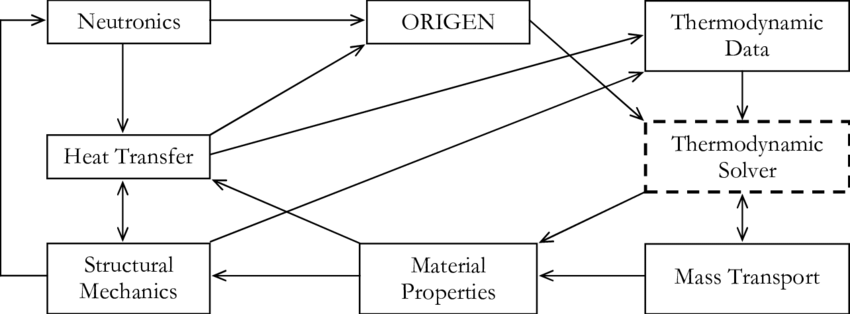
\includegraphics[width=0.75\textwidth]{figures/AMP_TC.png}
%		\caption[A flowchart of the Advanced Multi-Physics (AMP) code illustrating the interaction between the various modules.]{A flowchart of the Advanced Multi-Physics (AMP) code illustrating the interaction between the various modules is shown \cite{Piro11b}.}
%		\label{fig:amp}
%		\end{center}
%	\end{figure}
%	\begin{figure}[htb]
%		\begin{center}
%		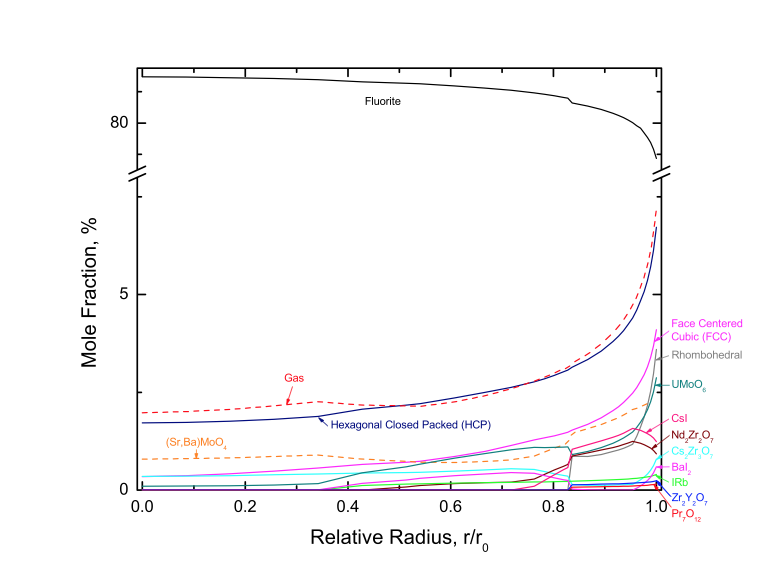
\includegraphics[width=0.85\textwidth]{figures/Piro_JNM}
%		\caption[The predicted distribution of phases across the pellet is shown for an average pellet burnup of 102 GW d t(U)$^{-1}$.]{The predicted distribution of phases across the pellet is shown for an average pellet burnup of 102 GW d t(U)$^{-1}$ \cite{Piro13b}.}
%		\label{fig:pirojnm}
%		\end{center}
%	\end{figure}

	The software integration of Thermochimica with Bison was performed by Simunovic et al. \cite{Simunovic:2020aa}. Use of Thermochimica was demonstrated by modelling oxygen transport in irradiated \ce{UO2} oxide fuel, such as calculation of oxygen to metal ratio in the fluorite phase, oxygen partial pressure, oxygen chemical potential and oxygen transport. Experimental measurements from the open literature were used to validate the implemented models and illustrate functionality of the developed thermodynamics module. The calculations are based on chemical element inventory provided by neutronics, isotopic depletion, transmutation and decay calculations in the \cite{SCALE05} system. To overcome some of the computational cost increase observed by Simunovic et al., Poschmann et al. used a reinitialisation strategy whereby the Thermochimica results were saved at each node at each time step and used to initialise the calculations at the next time step \cite{Poschmann:2019aa}. Poschmann et al. \cite{Poschmann:2021aa} extended the model by  Simunovic et al. to simulate the the \ce{U} and \ce{Zr} interdiffusion in \ce{U-Pu-Zr} metallic fuel. A similar effort by Hirschhorn et al. used Bison as well but with pre-computed thermodynamic values obtained from PyCalphad \cite{Hirschhorn:2021aa}. 

	In France, 3D coupled multiphysics simulations of power ramps in Pressurised Water Reactors (PWR) were performed by Baurens et al. \cite{Baurens:2014aa} and  Konarski et al. \cite{KONARSKI2019104}. The fuel performance code {ALCYONE}, which is part of the computing environment {PLEIADES}, was coupled with the thermodynamics code {ANGE} to provide a description of irradiated fuel thermochemistry with oxygen transport taking into account thermodiffusion. Konarski et al. also performed Pellet Cladding interaction (PCI) failure analyses \cite{Piro:2020aa}, by coupling thermochemistry and thermo-mechanics to investigate both chemical and mechanical factors simultaneously. 3D thermochemical-mechanical simulations of PWR power ramps on \ce{Cr}-doped \ce{UO2} with the fuel performance code {ALCYONE} including oxygen transport were performed to study the impact of oxygen redistribution on irradiated fuel thermochemistry and on chemically reactive fission gas release. OpenCalphad has been coupled with ALCYONE for several applications such as those by Michel et al. \cite{Michel:2013aa} and Intro\"{i}ni et al. Intro\"{i}ni et al. proposed multiple coupling strategies to improve the computational performance of the OpenCalphad - ALCYONE coupling and through a set of numerical experiments, demonstrated the performance gain compared to ANGE - ALCYONE coupling. Another code in the PLEIADES environment is GERMINAL which is specifically aimed at Sodium cooled fast reactor (SFR) and was coupled to OpenCalphad by Samuelsson et al. \cite{Samuelsson-Karl:2020aa} to model Joint Oxyde-Gaine (JOG) \cite{Gueneau:2020aa}.
	
	Use of thermodynamic equilibrium data finds a lot of value in phase field calculations where quantities like Gibbs energy, chemical potentials are all required as inputs. Among the first applications of such coupling were those in the field of metallurgy like those by Grafe et al. \cite{Grafe:2000aa} and Chen et al. \cite{Chen:2005aa} Several other models have been developed with some examples being of those by Zhang et al. \cite{Zhang:2015aa} who directly incorporated Calphad into the phase-field formalism and validated the coupling technique for \ce{Fe-C} and \ce{Ni-Al} alloys and by Schwen et al. \cite{Schwen:2017aa} who used PyCalphad for thermodynamic data in  MOOSE-based phase field application MARMOT. Schwen et al. have also developed a multiphase field model for better integration of thermodynamic phases with multiple sublattices in the phase field model implemented in MOOSE \cite{Schwen:2021aa}. Other similar works include those of B\"{o}ttger et al. \cite{Bottger:2020aa}, Chatterjee and Moelens \cite{Chatterjee:2021aa}, Zuo et al. \cite{Zuo:2021aa} and Coutinho et al. \cite{Coutinho:2022aa}.

	Among other applications, Poschmann et al. \cite{Poschmann:2022aa} coupled Thermochimica to dynamic systems modelling software TRANSFORM for dynamic mass accountancy in liquid-fuelled MSRs and  Fitzpatrick et al. \cite{Fitzpatrick18} coupled Thermochimica with thermal-hydraulics code COBRA-TF and isotopic evolution code ORIGEN to demonstrate fission product transportation by coolant flow in molten salt reactors. Thermochimica has recently been coupled with MELCOR for severe accident modelling in Boiling Water Reactors (BWR) \cite{Breeden:2022aa}.

	Thus, thermodynamic equilibrium calculations have found application in modelling and simulation several physical phenomena. Full integration of a thermodynamic equilibrium code in {MOOSE} would make such coupled calculations easy and allow high fidelity multiphysics simulations allowing much more realistic simulations of various problems. In doing so, however, one must be considerate of the increase in computational cost and should carefully do a cost-benefit analysis before proceeding with such high-fidelity but costly simulations.

\section{Summary}
    Computing thermodynamic equilibrium is a challenging problem and over the years a large number of software codes have been developed to tackle it. Most of these codes can be classified into three broad categories based on the numerical methods and the most popular numerical method has undoubtedly been White's method based on Lagrange multiplier which is now often described as the Gibbs energy minimisation method. Despite numerous codes existing in literature, there are several limitations that must be addressed as part of this work. Firstly, a majority of the codes are designed for small systems and mostly aimed at phase diagram construction. Secondly, until very recently only FactSage supported MQMQA and even now only Thermochimica and PyCalphad have added support for it. Thirdly, most of the codes have been designed as standalone applications instead of for coupling to other codes. Lastly, the state of global optimisation algorithms used in thermodynamic equilibrium is relatively simplistic. Most codes designed for general applications use simple sampling methods and the few codes which use better global optimisation algorithms are designed for very simple problems such as liquid vapour equilibrium. Furthermore, there's almost no systemic study of optimisation algorithms and their performance when applied to equilibrium problems of reasonable complexity. For any general thermodynamic equilibrium solver developed for multiphysics simulations, such as the one in this work, several of these limitations must be addressed. 
\chapter{Computational Implementation} \label{chap:implementation}

	The principles of thermodynamic equilibrium set the background for solving phase equilibrium problem in multicomponent system but being able to solve the resulting optimisation problem requires the use of high-quality software implementations. Though several such softwares exists, most of them do not meet the requirements for direct integration with MOOSE framework. The commercial softwares do not provide source codes and the application programming interfaces (APIs) provided by a few of such codes are usually very difficult to modify to meet the needs of multiphysics implementations. The open-source softwares on the other hand do have readily available source codes but often lack in terms of quality of code implementation and software quality assurance (SQA). To overcome the challenges and to provide readily usable thermodynamic equilibrium framework in MOOSE, a new Gibbs energy minimiser was developed.  While many of the algorithms employed in {\GEM} embody the concepts previously presented in open literature, there remains a scope for improving the efficiency and capabilities of some of these algorithms through careful implementation and/or building upon them. The top level architecture of the thermodynamic equilibrium solver has been outlined in figure~\ref{fig:structure}. The program essentially consists of parsing and input modules to read the required thermodynamic data and system information followed by initialisation routines which provide the initial assemblage to a non-linear solver. The assemblage from the non-linear solver is then checked to ensure global minimum is achieved at which stage the outputs are produced.
	\begin{figure}[htbp]
	 	\centering
	   	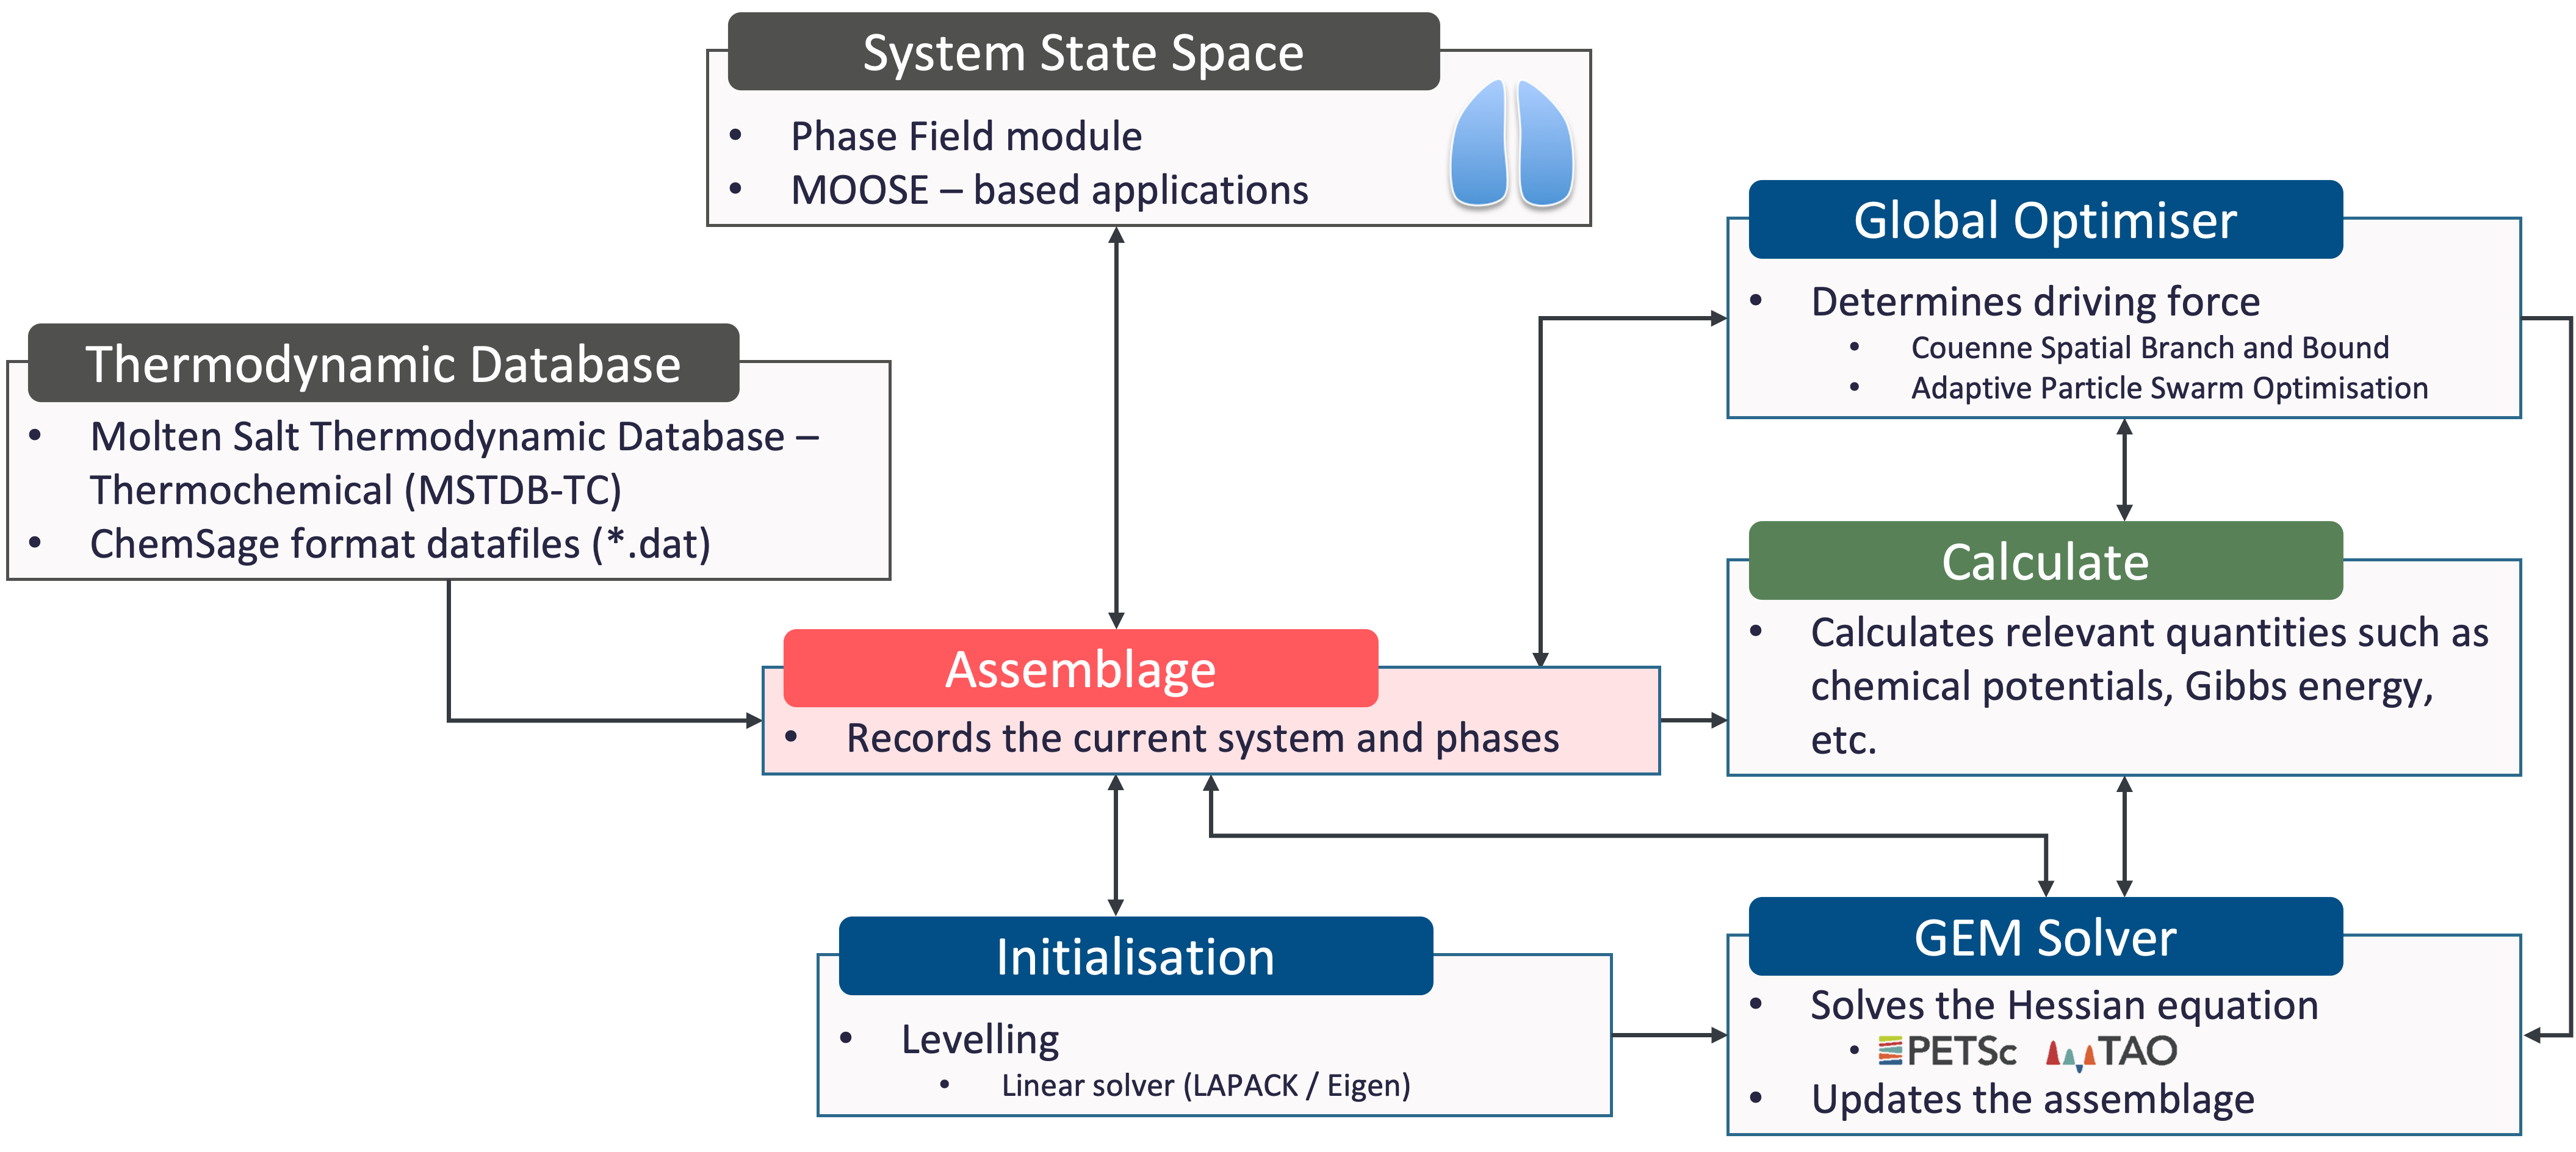
\includegraphics[width=0.95\textwidth]{figures/chapter-6/YJ_structure.png}
	   	\caption{Top-level architecture of \GEM.}
	   	\label{fig:structure}
	\end{figure}


\section{Thermodynamic Database}
	Calculation of thermodynamic equilibrium requires a thermodynamic database, which includes Gibbs energy functions of the different phases and species that can exist in the system. These thermodynamic databases are developed using the well established CALPHAD method \cite{Kaufman:1970aa} and are available in different formats, the most commonly used being ThermoCalc (*.tdb) and ChemSage (*.dat) datafile formats, which are generated by the commercial software ThermoCalc and FactSage, respectively. An example of a typical ChemSage datafile is shown in figure~\ref{fig:datfile} and consists of a header block followed by information blocks for every possible phase in the system.
	\begin{figure}[htbp]
	 	\centering
	   	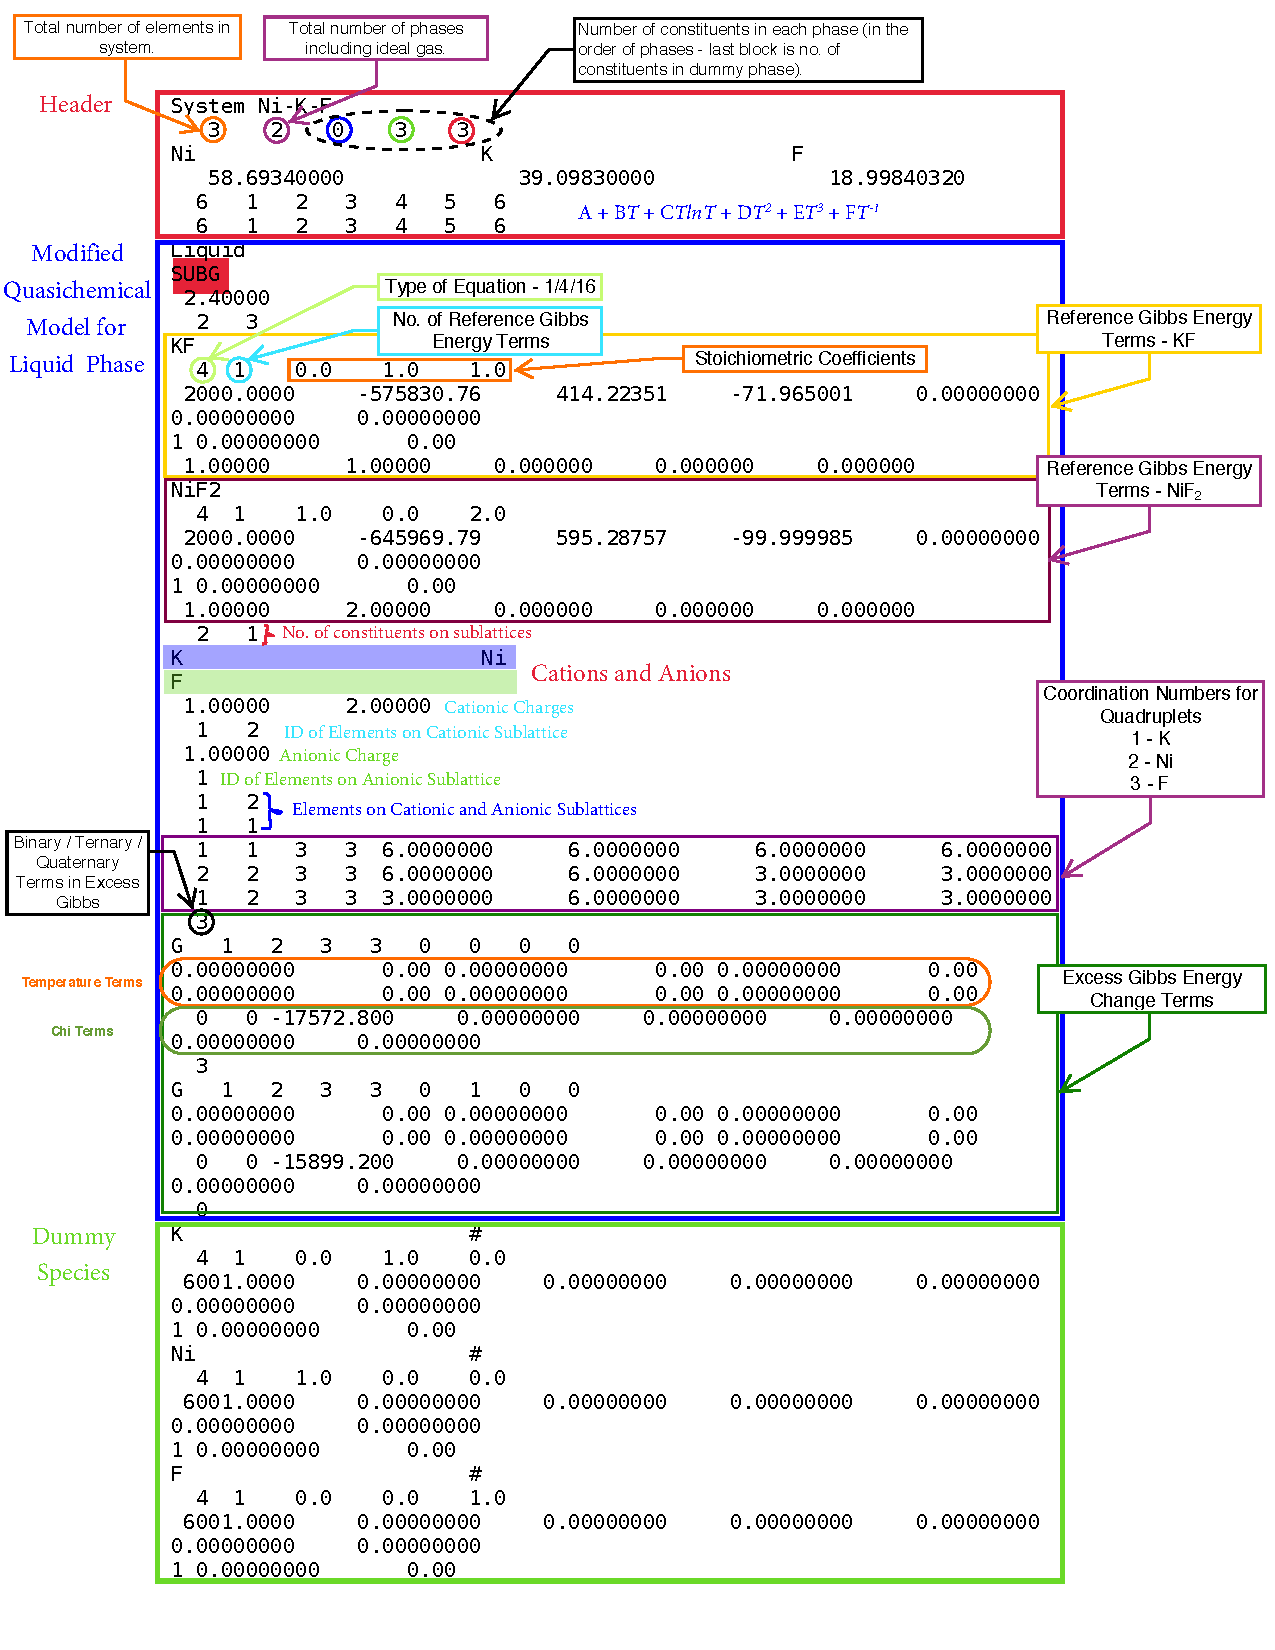
\includegraphics[width=\textwidth]{figures/chapter-6/NiKF.pdf}
	   	\caption[A marked-up example of a ChemSage datafile of the \ce{Ni-K-F} system.]{A marked-up example of a ChemSage datafile of the \ce{Ni-K-F} system \cite{OcadizFlores18}.}
	   	\label{fig:datfile}
	\end{figure}

	A datafile parser for {\GEM} has been developed in C++ and it performs the extraction of Gibbs energy functions from ChemSage format (*.dat) thermodynamic files and creates an in-memory thermodynamic database class, \texttt{Database}, that can be conveniently accessed by any part of the code throughout rest of the solve. All the data structure objects inherit from a single base class allowing the rest of the code to track the phases conveniently without having to track the model-specific  details. Moreover, in multiphysics simulations, it allows a single database instance to be created at the start of the simulations instead of the need of reading the datafile every time the information is needed. In {\GEM}, the Molten Salt Thermodynamic Database - Thermochemical \cite{Besmann:2021aa,Ard:2022aa}, is natively supported but any ChemSage format datafile can be supplied by the user.
	
	The \texttt{Database} class includes a number of utility functions for post-processing and cleaning up the raw database constructed after parsing. A peculiarity of ChemSage datafiles is how they denote phases that can have a miscibility gap. In ChemSage, such phases are denoted by adding a duplicate entry for a phase that is considered to have miscibility gaps. This has several disadvantages. First, this creates unnecessary duplication of thermodynamic data and can have memory and performance implications for large databases. Second, the decision for miscibility gap should be enforced using physical rules rather than basing them upon the database or user inputs. As an example, since a phase with more than one miscibility gap is not only plausible but also observed in many physical systems, a phase being duplicated once doesn't reveal any information about the number of such possible gaps and can be a source of confusion. In post-processing, such duplicate entries are deleted, but to not lose the information completely, a flag is raised in the thermodynamic phase whose duplicate was deleted. For multi-sublattice phases, the post-processor also maps all the sublattice constituents to the system components, and, for phase represented by MQM, it calculates the default coordination numbers for the quadruplets that are not included in the datafile.
	
\section{System State-Space}
	Thermochemical equilibrium calculations are isothermal, isobaric point calculations and require the temperature, pressure as well as the composition if the system to be specified. In {\GEM}, this information is provided by MOOSE or MOOSE-based applications such as the Phase Field module. To facilitate such data transfer, a MOOSE UserObject, namely \texttt{GEMUserObject}, has been developed. The MOOSE UserObject system is built for developing and running custom algorithms that may not fit well within any other system in MOOSE. Examples include complex calculations that may result values that don't associate in a one to one manner with elements, nodes, or sides. \texttt{GEMUserObject} allows the thermodynamic equilibrium solver to be called by other codes and the invocation requires that the temperature, pressure and composition be specified as required parameters. The UserObject is also responsible for passing back the return values to the calling code and some of the common variables that are often requested include the Gibbs energy, chemical potentials, stable phases and their speciation.

\section{Initialisation}
	Much like any other optimisation problem, the choice of initial estimate plays a critical role in reducing the amount of computational time required for the solution to converge to a minimum. This requirement of initial estimates of the stable  phases and their speciation creates a significant challenge. Many early softwares created for the purpose of estimating thermodynamic equilibrium, for example SOLGASMIX, required the user to input an initial estimate but this relied on the user's intuition and was often very inconvenient for them, especially when working with complex systems and/or systems where finding estimates from intuition was not straightforward. A bigger problem was that it could often result in initial estimates that were far from the real stable assemblage of phases and would increase the computational cost substantially, often even compromising the convergence itself. 

	To overcome the need for user prescribed initial estimates, Eriksson and Thompson \cite{Eriksson89} proposed an initialisation algorithm called \emph{levelling} that has found widespread application in thermodynamic equilibrium softwares. {\GEM} implements this algorithm as the standard initialisation routine and the it is described in the following text.
	
\subsection{Levelling}
	The levelling algorithm was developed to accelerate the rate of convergence by eliminating the phases and species that have an insignificant contribution in the final phase assemblage. The algorithm is based on a temporary treatment of all species and phases in the system as pure stoichiometric phases. Mathematically, this amounts to temporarily converting the non-linear optimisation problem into a linear optimisation problem and the algorithm for the computational implementation has been illustrated in figure~\ref{fig:levelling}.
	\begin{figure}[ht!]
		\centering
		\begin{tikzpicture}[auto,
    			block_center/.style ={rectangle, draw=black, thick, fill=white, text width=0.2\textwidth, text centered, minimum height=2em},
    			block_side/.style ={rectangle, draw=black, thick, fill=white, text width=0.2\textwidth, text centered, minimum height=2em},
			block_noborder/.style ={rectangle, draw=none, thick, fill=none, text width=0.15\textwidth, text centered, minimum height=0.5em},
			block_small/.style ={rectangle, draw=none, thick, fill=none, text width=0.1\textwidth, text centered, minimum height=0.5em},
			line/.style ={draw, thick, -stealth}]
    			% Outlining the flowchart using the PGF/TikZ matrix funtion
    			\matrix [column sep=0.15\textwidth,row sep=5em] {
      				{} & \node [block_center] (01) {Initial guess}; & {}\\
      				{} & \node [block_center] (11) {Calculate $\mu_i$ of species}; & {}\\
      				\node [block_side] (20) {Initial estimate found}; & \node [block_center] (21) {Levelling}; & \node [block_side] (22) {Calculate molar amounts};\\
      				{} & \node [block_center,yshift=-1cm] (31) {Exchange phase}; & {}\\
      				{} & \node [block_center] (41) {Compare to the list of previous assemblages}; & \node [block_side] (42) {Calculate chemical potential of component};\\
    			};	% end matrix
    			% connecting nodes with paths
    			\begin{scope}[every path/.style=line]
      				\path (01) edge (11);
     				\path (11) edge (21);
      				\path (21) edge node[block_noborder,anchor=east]{\footnotesize{Phase with most negative relative Gibbs energy}} (31);
      				\path (31) edge (41);
      				\path (22) edge node[block_noborder,anchor=south]{\footnotesize{All positive and real}} (21);
      				\path (21) edge node[block_noborder,anchor=south]{\footnotesize{All phases' Gibbs energies are positive}} (20);
      				\path (41) edge node[block_noborder,anchor=north]{\footnotesize{New assemblage}} (42);
      				\path (42) edge (22);
      				\path[-] (22.185) edge node[block_noborder,rotate=49.5,anchor=south]{\footnotesize{Negative or non-real numbers}} (31.5);
      				\path[-] (41.10) edge[bend right=60] node[block_small,anchor=west,shift={(-0.125cm,0)}]{\footnotesize{Already considered}} (31.355);
     				\path[-] (42.135) edge[bend right=37] node[block_small,anchor=west,shift={(0,0.225cm)}]{\footnotesize{Non-real numbers}} (31.360);
    			\end{scope}
 		\end{tikzpicture}
  		\caption[Levelling algorithm for finding the initial estimate of stable phase assemblage.]{Levelling algorithm for finding the initial estimate of stable phase assemblage. After Loukusa \cite{Loukusa:2014aa}.}
  		\label{fig:levelling}
 	\end{figure}

	Since the Gibbs energy is a relative thermodynamic function and the Gibbs energies of each component element are not related to one another \cite{Eriksson89}, it is possible to numerically alter the Gibbs energy of each phase while preserving the elemental differences. Levelling is performed by representing the set of Gibbs energies relative to the collection of phases assumed to be most stable and uses a relative Gibbs energy function called the \textit{absolute Gibbs energy} by Eriksson and Thompson and is the Gibbs energy of the pure species per atom in the species as shown in equation~\eqref{eq:absGibbs}
	\begin{equation}\label{eq:absGibbs}
		\hat{G}_i = \frac{G_j}{\sum_{j=1}^C \nu_{ij}}.
	\end{equation}

	The levelling process determines the combination of phases yielding the lowest Gibbs energy by evaluating a combination of Gibbs energies on a relative basis. A phase that has a negative relative Gibbs energy with respect to the assemblage indicates that a phase in the assemblage must be replaced by the current phase to achieve a lower integral Gibbs energy. Mathematically, levelling is achieved through an iterative process that systematically adjusts fixed combinations of phases, subject to the linear equality and inequality mass balance constraints, to progressively minimise the GIbbs energy of the system \cite{Piro12a}. At iteration $m+1$, the adjustment to be applied to the relative Gibbs energy of phase $i$ is defined by \cite{Eriksson89}:
	\begin{equation} \label{eq:lev_adj}
		\begin{aligned}
			d \hat{G}_i^{m\rightarrow m+1} &= \sum_{j=1}^{C} c_{ij} d \Gamma_j^{m\rightarrow m+1},\\
			\hat{G}_i^{m+1} &= \hat{G}_i^{m} - d \hat{G}_i^{m\rightarrow m+1},
		\end{aligned}
	\end{equation}
	where $c_{ij}$ denotes the atomic fraction of element $j$ in species $i$ and $d \Gamma_j^{m\rightarrow m+1}$ is the adjustment applied to the chemical potential of element $j$, which in turn is determined by the most stable phases found at iteration $m$. In  matrix form, the overall mass balance constraint can be represented as \cite{Piro12a}
	\begin{equation} \label{eq:levMB_mat}
		\mathbf{A^T} \mathbf{n}= \mathbf{b},
	\end{equation}
	where $\mathbf{A} \in \mathbb{R}^{E \times \Phi}$ represents the stoichiometric matrix, $\mathbf{n} \in \mathbb{R}^{\Phi }$ denotes the column vector of the number of moles of each phase, and $\mathbf{b} \in \mathbb{R}^{E}$ is the column vector with the total mass of each element in the system. When equation~\ref{eq:levMB_mat} is used in levelling, $\Phi = E$.

	The initial guess for the levelling method is the most chemically stable form of each element and the stoichiometric matrix $\mathbf{A^T}$ in equation~\eqref{eq:levMB_mat} becomes a diagonal matrix. Subsequently, provided all elements of vector $\mathbf{b}$ are positive, all the elements of $\mathbf{n}$ must also be positive. However, the diagonality of the stoichiometric matrix is not preserved over subsequent iteration and it assumes a non-symmetric sparse form. In fact, the matrix $\mathbf{A^T}$ might become rank deficient if proper care is not taken while selecting the phase assemblage.

	In levelling, since the number of phases in the system is equal to the number of elements, the element potentials can then be uniquely determined from the current estimated phase assemblage by solving the following system of linear equations:
	\begin{equation} \label{eq:levEP_mat}
		\mathbf{A^T} \boldsymbol{\Gamma} = \boldsymbol{\mu},
	\end{equation}
	where $\boldsymbol{\Gamma} \in \mathbb{R}^{E} $ and $\boldsymbol{\mu} \in \mathbb{R}^{\Phi}$.

	The next step in levelling is updating the phase assemblage in accordance with equation~\eqref{eq:lev_adj}. A  species with a positive $\hat{G}_i^{m+1}$ would yield a thermodynamically less stable assemblage and is left out along with phases with insignificant contributions to final equilibrium while the phase with the most negative $\hat{G}_i^{m+1}$ is introduced into the assemblage by replacing a phase in the previous assemblage. The phase assemblage at this stage must meet three requirements. First, the number of moles of all phase in $\mathbf{n}$ must be non-negative and real. Second, all the elements of the vector $\boldsymbol{\Gamma}$ must be real. Finally, the phase assemblage must not have been previously considered. If the phase assemblage does not meet any of these requirements, the phase with the second lowest relative Gibbs energy must be considered, and so on.

	While the criteria for the phase to be added in the system was well established by Eriksson and Thompson, a criterion to select the phase to be replaced wasn't proposed and, typically, local iterations were performed to systematically traverse through the candidate phases until a particular combination yielded an entire set of non-negative and real mole numbers \cite{Eriksson89}. The number of these local iterations rapidly grows with the number of elements in the system and an alternative named \emph{Euclidean norm} was proposed by Piro and Simunovic \cite{Piro12a}. This method has been described in section~\ref{sec:Euclidean}.

	Once the new phase has been exchanged with one of the existing phases and its acceptability has been determined, levelling step is repeated until no phases with negative absolute Gibbs energy remain in the system. At this stage, the assemblage can be passed on to a non-linear solver as the initial estimate.
	\begin{figure}[ht]
		\centering
		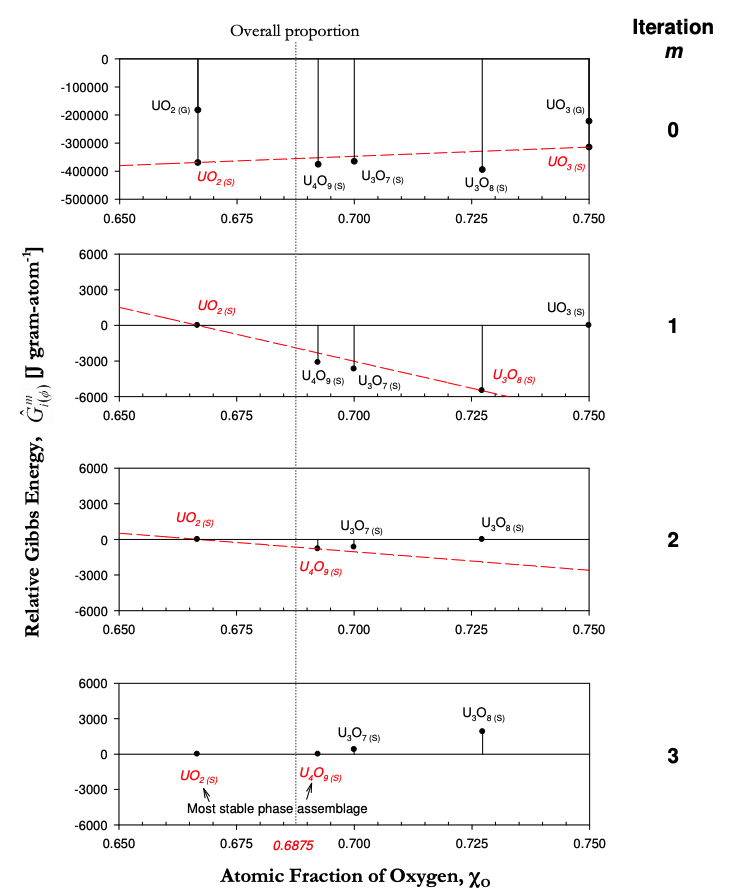
\includegraphics[width=\textwidth]{figures/chapter-6/Levelling_illustration}
		\caption[Illustration of the levelling process for a binary system of \ce{U-O} at each iteration (1 \si{\mole} \ce{U}, 2.2 \si{\mole} \ce{O}, 298.15 \si{\kelvin}, 1 \si{atm}).]{Illustration of the levelling process for a binary system of \ce{U-O} at each iteration (1 \si{\mole} \ce{U}, 2.2 \si{\mole} \ce{O}, 298.15 \si{\kelvin}, 1 \si{atm}). From Piro et al. \cite{Piro11b}.}
		\label{fig:lev_illus}
	\end{figure}

	An example of the levelling method is presented in figure~\ref{fig:lev_illus}. In the illustration, in the first iteration, the phase with the most negative Gibbs energy is paired with another phase that together has non-negative molar quantities. At the end of iteration 0, choosing solid \ce{UO2} as the phase with the most negative relative Gibbs energy and arbitrarily choosing solid \ce{UO3} to pair it with, the equivalent Gibbs energies of pure uranium and pure oxygen are computed and followed by the element potentials $\Gamma_{\ce{U}}$ and $\Gamma_{\ce{O}}$ (represented by the dashed red line). The levelling procedure is then applied and the relative Gibbs energies of the terms are calculated.

	At the start of iteration 1, the relative Gibbs energy of solid \ce{U3O8} is negative with respect to the combination of solid \ce{UO2} and solid \ce{UO3}, indicating it must be introduced in the assemblage. The internal linear solver then determines the phase that must be replaced and the iterative process continues with the updated phase assemblage.

	At the end of the levelling procedure, the assemblage has the lowest Gibbs energy with all other phases being positive with respect to the assemblage. The Gibbs energy of the pure stoichiometric system is thereby minimised. For the example presented in figure~\ref{fig:lev_illus}, the levelling solver converges in only 3 iterations. According to Eriksson and Thompson \cite{Eriksson89}, the computational expense using levelling can be up to two to five times lower than the general equilibrium calculations.

	Mathematically, the levelling  process always respects the Gibbs phase rule, mass balance and the Gibbs' criterion and the number of iterations required to achieve convergence is typically close to the number of elements. This results in significant computational advantage when considering exceeding large number of possible phase combinations as the number of elements in the system grow making levelling an excellent choice as an initialisation routine.

\subsection{Euclidean norm} \label{sec:Euclidean}
	The Euclidean norm method was proposed by Piro and Simunovic \cite{Piro12a}, to strategically rank the best candidate phases to accommodate a new phase change. The Gibbs phase rule requires that when the thermodynamic degree of freedom $F$ equals zero, a phase must be removed in order to introduce a new phase. Determining whether a candidate phase is feasible is the most expensive task within the global iteration cycles as it requires solution of a simultaneous equation to ensure that the Hessian matrix is non-singular \cite{Piro12a}. If there are multiple candidate phases, this iterative process must be repeated for each candidate.

	The Euclidean norm method systematically ranks the best candidates to be withdrawn from the system without having to perform an exhaustive search. The method is based on the principle that the best candidate phase to be withdrawn from the current assemblage has the most similar atomic composition to the phase that has to be added to the system. The atomic fractions in phase $\phi$ are represented by the following equation:
	\begin{equation}
		c_{\phi j} = \frac{\sum_{i=1}^{N_{\phi}} \nu_{ij}}{\sum_{i=1}^{N_{\phi}} \sum_{k=1}^{C} x_i \nu_{ik}},
	\end{equation}
%	
%
%	The atomic fraction of element $j$ in a pure stoichiometric phase $\omega$ is represented as:
%	\begin{equation}
%		c_{\omega j} = \frac{c_{\omega j}}{\sum_{k=1}^{E} x_{i(\omega)}\nu_{\omega j}}
%	\end{equation}
%
%	Similarly, in the solution phase  $\lambda$, the atomic fraction of element $j$ is computed by
%	\begin{equation}
%		c_{\lambda j} = \frac{\sum_{i=1}^{N_{\lambda}} \nu_{ij}}{\sum_{i=1}^{N_{\lambda}} \sum_{k=1}^{E} x_{i(\lambda) \nu_{ik}}}
%	\end{equation}

	Denoting the atom fraction of the element $j$ in the new phase that is to be introduced into the system with $c_{\phi j}^{*}$, the difference between this phase and the phases currently in the assemblage is given by the Euclidean norm of each phase $\phi$
	\begin{equation}
		\|c_\phi\|_2 = \sqrt{\sum_{j=1}^{E} \left(c_{\phi,j} - c_{\phi,j}^{*}\right)^2}.
	\end{equation}

	The phase with the lowest Euclidean norm has the most similar composition to the phase to be introduced in the assemblage. In case the resulting assemblage does not meet the criterion to be a valid assemblage, the phase with the second lowest Euclidean norm can be introduced and so on.

\section{Non-linear solver}
	The linear solver can often provide estimates close to the final assemblage of the system and in certain circumstances, such as for systems with only pure 	stoichiometric species, it might be able to predict the equilibrium assemblage. However, almost always, further computations are required to arrive at the final assemblage especially in cases where the phases have more than one species with significant contribution to the Gibbs energy. This situation arises more often than not and a non-linear solver is required to handle the non-linearities arising from the logarithmic term in the compositional component of the chemical potentials.

	For the sake of completeness of the argument, the conditions for equilibrium are restated below:
	\begin{enumerate}
		\item The mass balance constraint must be satisfied.
		\item The Gibbs' phase rule must be satisfied.
		\item The integral Gibbs energy must be at a global minimum.
	\end{enumerate}

	The following subsidiary conditions arise from the constraints
	\begin{enumerate}[label=\Alph*.]
		\item The number of moles of any species must be positive.
		\item The sum of mole fractions must be one (inherent in the Gibbs energy method).
	\end{enumerate}
	
	\subsection{Numerical implementation}
	The system of non-linear equations can be solved using the Newton-Raphson method. Newton-Raphson method depends on solving equation~\eqref{eq:GEM_mat} and is an $\mathit{O}(N^3)$ operation where $N$ is the size of the system. 
	An integral component of the solver is an appropriate line-search algorithm to determine how far the system should progress along the direction vectors. The functional norm of the Lagrangian is an effective choice to ensure convergence and is defined as \cite{Piro17}:
	\begin{equation}
	\begin{aligned}
		\|f\|^2 = &\sum_{j=1}^{C}\left(\sum_{\lambda=1}^{\Lambda} n_\lambda \sum_{i=1}^{N_\lambda} x_{i(\lambda)}\nu_{ij} + \sum_{\omega=1}^{\Omega}n_{\omega}\nu_{\omega,j} - b_j\right)^2 \\
		&+ \sum_{\lambda=1}^{\Lambda} \left(\sum_{i=1}^{N_\lambda} x_{i(\lambda)}\left\vert\mu_{i(\lambda)} - \sum_{j=1}^{C}\nu_{ij} \Gamma_j \right\vert \right)^2 + \sum_{\omega=1}^{\Omega}\left(g_\omega - \sum_{j=1}^{C}\nu_{\omega,j} \Gamma_j \right)^2,
		\end{aligned}
	\end{equation}
	where the first term on the right represents the mass balance residuals, the second represents the absolute sum of chemical potential residuals of solution species and the third represents the chemical potential residuals of stoichiometric phases. By enforcing the Wolfe/Armijo condition \cite{Nocedal06}, a sufficient step length is decided.

	Each iteration step in the minimisation problem involves approximately solving the subproblem:
	\begin{equation}
		\min_\alpha f\left(\mathbf{x}^m + \alpha \mathbf{p}^m\right),
	\end{equation}
	where $\mathbf{x}^m$ is the best estimate at iteration $m$, $\mathbf{p}^m$ denotes the search direction vector and $\alpha$ represents the step size.

	The Wolfe conditions are a set of inequalities for performing inexact line search and provide an efficient way of computing an acceptable step length $\alpha$  that reduces the objective function sufficiently, rather than minimising the objective function over $\alpha \in \mathbb {R}^{+}$ exactly.

	A step length $\alpha^m$ is said to satisfy the Wolfe conditions, restricted to the direction $\mathbf{p}^m$, if the following two inequalities hold:
	\begin{equation}
		f\left(\mathbf{x}^m + \alpha^m \mathbf{p}^m\right) \leq f\left(\mathbf{x}^m \right) + c_1 \alpha^m \left(\mathbf{p}^m\right)^T \nabla f\left(\mathbf{x}^m \right),
	\end{equation}
	\begin{equation}
		- \left(\mathbf{p}^m\right)^T \nabla f\left(\mathbf{x}^m + \alpha^m \mathbf{p}^m\right) \leq - c_2 \left(\mathbf{p}^m\right)^T \nabla f\left(\mathbf{x}^m \right),
	\end{equation}
	with $0 < c_1 < c_2 < 1$. The first inequality, known as the Armijo condition ensures that the step length $\alpha^m$ decreases $f$ sufficiently, and the second inequality known as the curvature condition ensures that the slope has been reduced sufficiently. Together, the two inequalities provide upper and lower bounds for the step lengths \cite{Nocedal06}.
	
	{\GEM} uses the state-of-the-art non-linear solvers in PETSc to solve the non-linear system. The \texttt{SNESNEWTONLS} is a Newton based nonlinear solver that uses line search and has been used as the default solver in this work. 
	
	
\subsection{Adding/Removing phases}
		Updating the estimated phase assemblage plays a significant role in the convergence of thermodynamic solvers. Inadequate strategies for updating the assemblage might lead to inefficient global iterations (i.e., iterations in which changes are made to the system such as addition/removal of phases while the Newton iterations described above can be referred to as local iteration since they are aimed at finding the minimum of a problem with a fixed system) and might even prevent convergence. Though the number of phases that can be added into or removed from the system is constrained by the Gibbs' phase rule, proper care must be taken to ensure that any change to the system drives it towards convergence and not hold it back. To ensure that the phase assemblage updating does not result in undesired behaviour, the strategy proposed by Piro \cite{Piro17} has been adopted. This strategy has been illustrated in figure~\ref{fig:assemblage}.
\newgeometry{margin=1cm}
\begin{landscape}
\thispagestyle{empty}

		\begin{figure}[ht]
		\centering
		\begin{tikzpicture}[auto,
    			block_center/.style ={rectangle, draw=black, thick, fill=white, text width=0.25\textwidth, text centered, minimum height=2em},
    			block_side/.style ={rectangle, draw=black, thick, fill=white, text width=0.15\textwidth, text centered, minimum height=2em},
			block_noborder/.style ={rectangle, draw=none, thick, fill=none, text width=0.15\textwidth, text centered, minimum height=0.5em},
			block_small/.style ={rectangle, draw=none, thick, fill=none, text width=0.1\textwidth, text centered, minimum height=0.5em},
			line/.style ={draw, thick, -stealth}]
    			% Outlining the flowchart using the PGF/TikZ matrix funtion
    			\matrix [column sep=10em,row sep=5em] {
      				\node [block_center] (00) {Initial assemblage from GEM solver}; & {} \\
      				\node [block_center] (10) {Phase to be removed?}; & \node [block_center] (11) {Phase to be added?}; \\
				\node [block_center] (20) {Remove phase}; & \node [block_center] (21) {Rank candidates using euclidean norm}; & {}\\
				\node [block_center] (30) {Retest new assemblage}; & \node [block_center] (31) {Exchange phases}; & \node [block_center] (32) {Add new phase};\\
				\node [block_center] (40) {Exchange phases}; & \node [block_center] (41) {Retest new assemblage}; & {} \\
				{} & \node [block_center] (51) {\textbf{Assemblage found}}; & {}\\
    			};	% end matrix
    			% connecting nodes with paths
    			\begin{scope}[every path/.style=line]
      				\path (00) edge (10);
     				\path (10) edge node[block_noborder,rotate=90,anchor=south]{\footnotesize{Yes}} (20);
				\path (10) edge node[block_noborder]{\footnotesize{No}} (11);
				\path (20) edge (30);
				\path (30) edge node[block_noborder,rotate=90,anchor=south]{\footnotesize{Failed}} (40);
%				\path (30.360)[-] edge node[block_noborder]{\footnotesize{Passed}} (51.180);
				\path (30.360) -- +(4em,0) |- node[block_noborder,rotate=90,anchor=south west,xshift=2.5em]{\footnotesize{Passed}} (51.180);
				\path[-] (40.180) edge[bend left] (30.180);
				\path (11) edge (21);
				\path (21) edge node[block_noborder,anchor=west,xshift=-0.5em]{\footnotesize{Can't add directly}} (31);
				\path (21.360) -| node[block_noborder,anchor=north east,xshift=-2.5em]{\footnotesize{Can add directly}} (32.90);
				\path (31) edge (41);
				\path (32.270) |- (41.360);
				\path[-] (41.180) edge[bend left] node[block_noborder,rotate=90,anchor=south]{\footnotesize{Failed}}(31.180);
				\path (41) edge node[block_noborder,rotate=90,anchor=south]{\footnotesize{Passed}}(51);
			\end{scope}
 		\end{tikzpicture}
  		\caption[Illustration of the methodology for updating the phase assemblage.]{Illustration of the methodology for updating the phase assemblage. Adapted from Piro \cite{Piro17}.}
  		\label{fig:assemblage}
	\end{figure}

\end{landscape}
\restoregeometry

\subsection{Convergence criterion}
	The convergence of the solver is tested in accordance with conditions for convergence described in chapter~\ref{chap:equilibrium}. The relative error of the mass balance and Gibbs' criterion is calculated  and the solver converges when both of these are within the specified tolerance. In addition, it must be tested that the mole numbers are not negative for any species in the system. The charge neutrality constraint must also be respected.  To minimise the computational cost, it is also possible to test convergence only when the functional norm has been satisfied to a specified tolerance.

	Two issues that can prevent convergence were foreseen for a thermodynamic equilibrium solver. First, when the objective function has multiple roots, for example due to miscibility gap, and second when the slope of the objective function is extremely small or zero. These two issues can result in non-real numbers or divergence and possible failure of the iterative solver.
The numerical dampening through Wolfe/Armijo conditions and the use of levelling as an initialisation method helps in avoiding the ill-behaviour and promotes numerical stability and enhances performance characteristics. The proposed algorithm of the thermodynamic solver with both local and global iterations has been presented in figure~\ref{fig:gem_illus}.
\newgeometry{margin=1cm}
\begin{landscape}
\thispagestyle{empty}

	\begin{figure}[ht]
		\centering
		\begin{tikzpicture}[auto,
    			block_center/.style ={rectangle, draw=black, thick, fill=white, text width=0.25\textwidth, text centered, minimum height=2em},
    			block_side/.style ={rectangle, draw=black, thick, fill=white, text width=0.15\textwidth, text centered, minimum height=2em},
			block_noborder/.style ={rectangle, draw=none, thick, fill=none, text width=0.15\textwidth, text centered, minimum height=0.5em},
			block_small/.style ={rectangle, draw=none, thick, fill=none, text width=0.1\textwidth, text centered, minimum height=0.5em},
			line/.style ={draw, thick, -stealth}]
    			% Outlining the flowchart using the PGF/TikZ matrix funtion
    			\matrix [column sep=2em,row sep=2em] {
      				\node [block_center] (00) {Initial estimate}; & {} & {} \\
      				\node [block_center] (10) {Calculate activities}; & \node [block_center] (11) {Calculate numbers of phase and species}; & {}\\
				\node [block_center] (20) {Calculate chemical potentials}; & {} & \node [block_center,yshift=-3em] (22) {Check if the phase assemblage is new};\\
				\node [block_center] (30) {Construct and solve linear system}; & \node [block_center,xshift=-7.5em] (31) {\textbf{Minimum Found}}; & {}\\
				\node [block_center] (40) {Calculate new mole amounts}; & \node [block_center,xshift=-7.5em] (41) {Correct mixture phase mole amounts}; & \node [block_side,xshift=-5em] (42a) {Add the phase};  \node [block_side,xshift=5em,yshift=-2.5em] (42b) {Select phase to be exchanged}; \node [block_side,xshift=5em,yshift=2.5em] (42c) {Exchange the phases};\\
				\node [block_center,yshift=-2.5em] (50) {Correct mole amounts}; & \node [block_center,yshift=-5em] (51) {Remove phases if possible}; & \node [block_center,yshift=-5em] (52) {Test if addition breaks Gibbs' phase rule};\\
				\node [block_center,yshift=-2.5em] (60) {Test convergence}; &  \node [block_center,yshift=-2.5em] (61) {Test if a phase should be added}; & \node [block_center,yshift=-2.5em] (62) {Select the best phase to be added};\\
    			};	% end matrix
    			% connecting nodes with paths
    			\begin{scope}[every path/.style=line]
      				\path (00) edge (10);
     				\path (10) edge (20);
				\path (20) edge (30);
				\path (30) edge (40);
				\path (40) edge (50);
				\path (50) edge node[block_noborder,anchor=east]{\footnotesize{No negative/small mole amounts, no NaN}} (60);
				\path (60) edge node[block_noborder,anchor=north]{\footnotesize{Converged}} (61);
				\path (61) edge node[block_noborder,anchor=north]{\footnotesize{Phase should be added}} (62);
				\path (62) edge (52);
				\path (61) edge node[block_noborder,anchor=west]{\footnotesize{No phase to add}} (51);
				\path[-] (51.90) edge node[block_noborder,anchor=east]{\footnotesize{No phase to remove}} (41.270);
				\path (41) edge  (31);
				\path[-] (51.20) edge node[block_noborder,anchor=south,rotate=90]{\footnotesize{Phase  removed}}(11.330);
				\path[-] (60.180) edge[bend left=20] node[block_noborder,anchor=north,rotate=90]{\footnotesize{Not converged}} (10.180);
				\path[-] (50.360) edge node[block_noborder,anchor=north,yshift=-0.25cm]{\footnotesize{Negative/small mole amounts or NaN}} (51.180);
				\path[-] (52.90) edge node[block_noborder,anchor=east]{\footnotesize{Phase rule satisfied}}(42a.270);
				\path[-] (52.90) edge node[block_noborder,anchor=west]{\footnotesize{Phase rule broken}}(42b.270);
				\path (42b) edge  (42c);
				\path[-] (42c.90) edge  (22.280);
				\path[-] (42a.90) edge  (22.260);
				\path[-] (22.90) edge node[block_noborder,anchor=west]{\footnotesize{New assemblage}}(11.360);
				\path (11) edge  (10);
				\path[-] (22.180) edge[bend right=30] node[block_noborder,anchor=south,rotate=90]{\footnotesize{Already tested}} (62.175);
			\end{scope}
 		\end{tikzpicture}
  		\caption[Illustration of the Gibbs energy minimisation algorithm.]{Illustration of the Gibbs energy minimisation algorithm. After Loukusa \cite{Loukusa:2014aa}.}
  		\label{fig:gem_illus}
	\end{figure}

\end{landscape}
\restoregeometry


\subsection{Interpreting the results}\label{sec:interpret_res}
	Though the developed algorithms are relatively very robust, there are certain classes of problems where the rank-deficiency in the stoichiometric matrices is inherent. In such cases, special care must be taken in interpreting the results computed by thermodynamic equilibrium codes. The author of this thesis co-authored a letter to the editor of Journal of Nuclear Materials explaining how one must be careful in interpreting the chemical potentials for molten salts systems. The letter by Piro et al. illustrates the case of a rank-deficient stoichiometric matrix in a model represented by MQMQA and shows how the chemical potential results can be misinterpreted. The author of this thesis contributed to the discussion presented in the work and co-authored the manuscript. 
	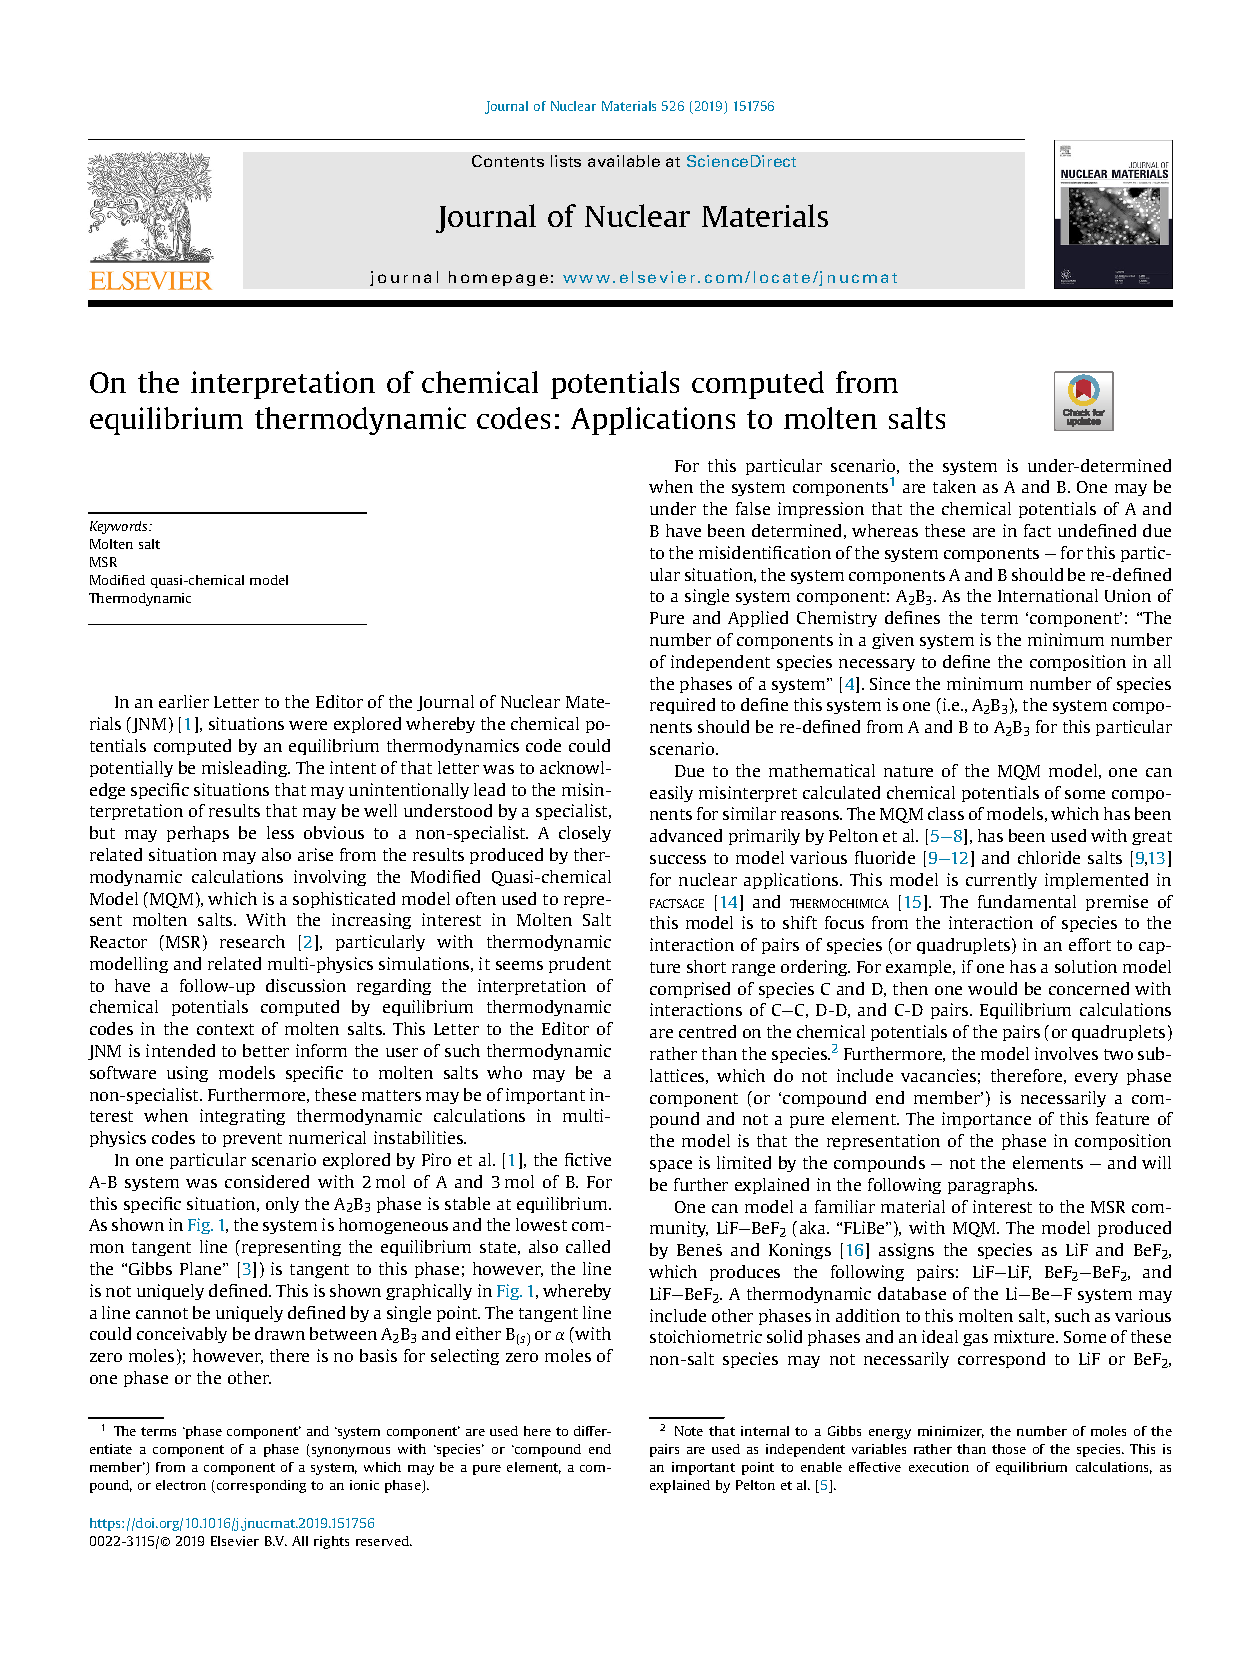
\includepdf[pages=-]{publications/Piro_2019.pdf}
	
%==============================================================================================================================
%														Global Optimisation
%==============================================================================================================================
\section{Global Optimisation}
%Ensuring that the global minimum of Gibbs energy is correctly calculated requires that the driving force of all metastable phases be positive. As described in section~\ref{sec:global_opt_intro}, computing the minimum driving force of a thermodynamic system requires solving a non-convex constrained optimisation problem. 
%
%	The computation of thermodynamic equilibrium, as discussed in sec.~\ref{sec:opt_theory}, is a global optimisation problem where the focus is on systems that can attain equilibrium state under conditions of constant temperature and pressure, where the global minimum value of the Gibbs energy describes the true equilibrium state. The problem can be stated as follows \cite{Floudas99}:
%	\begin{objective}
%	Given $C$ components participating in up to $\Phi$ potential phases under isothermal and isobaric conditions find the mole vector $\mathbf{n}$ that minimises the value of the Gibbs energy while also satisfying the appropriate material balance constraints.
%	\end{objective}
%
%	\begin{constraint}
%		The mole fraction of a species in phase $\lambda$, $x_{i(\lambda)}$, must satisfy the following linear equality and inequality constraints
%		\begin{equation}
%		\sum_{i=1}^{N_\lambda} x_{i(\lambda)} = 1 \mspace{30mu}x_{i(\lambda)} > 0\mspace{30mu} \forall i
%		\end{equation}
%	\end{constraint}
%
%The component set is represented by the index set $C = \{i\}$ and the elements that constitute these components are given by $E  = \{e\}$. The set of phases is denoted by $\Phi = \{k\}$ where it is composed of solution and stoichiometric phases, labelled $\Lambda$ and $\Omega$ respectively, so that $\Phi \equiv \Lambda\cup \Omega$.

	As described in section~\ref{sec:global_opt_intro}, computing the minimum driving force of a thermodynamic system requires solving a non-convex constrained optimisation problem. The conditions for thermodynamic equilibrium discussed in section~\ref{sec:eqb_theory} require that the chemical potentials of all the species must lie on or above the Gibbs plane, which passes through the element potentials $\Gamma_j$. Thus metastable phases must lie above the Gibbs plane and the difference between the Gibbs plane and the plane tangent to a metastable phase is referred to as the \emph{driving force} \cite{Lukas07} or \emph{tangent plane distance function} \cite{Lukas07,Zhang11}. The driving force for phase $\phi$ is represented by $\Delta G_{\phi}$ and is computed as \cite{Piro16}:
	\begin{equation}\label{eq:drivingforce}
        		\Delta G_{\phi}= \min_{\lambda} \sum_{i=1}^{N_{\lambda}}x_{i} \left (\mu_{i} - \sum_{j=1}^C \nu_{ij}\Gamma_j \right ),
    	\end{equation}
	which is subject to conservation of mass and the following linear equality and inequality constraints:
	\begin{align}
		\sum_{i=1}^{N_\phi} x_i = 1, \; x_i > 0, \; \forall i \in \phi.
	\end{align}
	The sufficient condition for equilibrium requires that the driving force $\Delta G_{\phi}$ computed with equation~\eqref{eq:drivingforce} is positive for all phases believed to be metastable and zero for all the stable phases. According to Hillert \cite{Hillert81}, the driving force of metastable phases can be evaluated at each iteration to determine whether or not it should be added into the system. However, this function can be non-convex and requires the evaluation of a global minimum. Though the open literature on computing these methods appears rather exhaustive, few authors have discussed generalised global minimisation schemes for the phase equilibria problem. The majority of articles focus either on relatively small systems, such as liquid-vapour equilibria, or are aimed at only a handful of calculations. Some notable exceptions to this include those of Hillert \cite{HILLERT198131}, Lukas et al.\cite{LUKAS1982229}, Sundman \cite{Sundman15}, Piro and Simunovic \cite{Piro16}, and Otis et al. \cite{Otis:2017ab}. Since both the robustness and computational efficiency of {\GEM} are of concern, a number of global optimisation methods were tested through a set of carefully constructed test problems representative of some common scenarios in equilibrium thermodynamics. Though no global optimisation method can guarantee the ability to find the true global minimum, sufficient confidence can be achieved for the problem under consideration under well-defined parameters.
	
	\subsection{Test Problems} \label{sec:test_global}
	To objectively test the reliability and performance of various global optimisation algorithms, the methods must be benchmarked against a set of test problems representative of the requirements from the solver. While most of the open  literature focusses on a single problem and tries to optimise the algorithm for the problem, such an approach is not ideal for the development of {\GEM}. Instead the focus here has been to select an algorithm that can work reasonably well for wide variety of problems with a large number of components. The reasoning behind such an approach is that a wide variety of excess mixing models are encountered in computational thermodynamics applied to nuclear materials. To test the algorithms under consideration, eight test cases representing different thermodynamic models and system sizes, and are summarised in table~\ref{tab:test_cases}.
	\begin{table}[htbp]
		\centering
	   	\caption{Summary of test cases used for comparing global optimisation algorithms.}
	   	\begin{tabular}{@{} lcp{0.82\linewidth} @{}} % Column formatting, @{} suppresses leading/trailing space
	      		\toprule
	      		\textbf{Label}	& \textbf{Size}		& \textbf{Problem Description} \\
	      		\midrule
	      		A			& 2					& Fictive binary system with a miscibility gap and a stoichiometric phase from Piro and Simunovic \cite{Piro16}.\\
	      		B			& 2					& \ce{Pd-Rh} binary system with a shallow FCC miscibility gap phase from Kaye \textit {et al.} \cite{Kaye07}.\\
	      		C			& 2					& Fictive binary system with three convex phases with one phase having a negative driving force from Piro and Simunovic \cite{Piro16}. \\
	      		D			& 3					& \ce{Pu-U-O} ternary system from Gu\'{e}neau et al. \cite{Gueneau11} containing an ideal gas phase, a non-ideal liquid phase, many stoichiometric phases and a \ce{(U$_y$ Pu$_{1-y}$)O$_{2\pm x}$} fluorite phase. Involves a multi-sublattice model and a charge balance constraint.\\
	      		E			& 3					& \ce{Al-Cr-Co} ternary system used as reference problem by Otis \textit {et al.} \cite{Otis:2017ab}. \\
	      		F			& 5					& Hexagonal closed packing (HCP) phase in the quinary system containing noble metal fission products \ce{Mo-Pd-Tc-Ru-Rh} from Kaye \textit {et al.} \cite{Kaye07}.\\
	      		G			& 10					& \multirow{2}{=}{Fictive high-dimensional systems with minefield of miscibility gaps based on Piro and Simunovic \cite{Piro16}.}\\
	      		H			& 30					& \\
	      \bottomrule
	   \end{tabular}
	   \label{tab:test_cases}
	\end{table}
	
	\begin{enumerate}
	\item	\emph{Problem A}\\
		A fictive binary  \ce{A-B} system based on Piro and Simunovic \cite{Piro16} has been considered as the first test problem. As shown previously in section~\ref{sec:global_opt_intro}, it consists of solution phase $\alpha$ and a stoichiometric phase \ce{A3B2} which can possibly coexist and while the stoichiometric phase \ce{A3B2} and solution phase $\alpha$ are initially predicted to be stable, as represented by the dashed tangent line in figure~\ref{fig:testA}, they are in fact metastable and a miscibility gap would yield a lower value of the integral Gibbs energy of the system, $G_\text{sys}$. The $\alpha$ phase is represented by a substitutional solution model with the reference Gibbs energies of the components being $g_{\ce{A}}^\circ = -100 $ \si{\joule \per \mole}, $g_{\ce{B}}^\circ = -300$ \si{\joule \per \mole} and the excess energy given by $g_{\alpha}^\text{ex} = 21000 x_{\ce{A}} x_{\ce{B}} + 7000 x_{\ce{A}} x_{\ce{B}}^2$. The temperature of the system was fixed at $T = 1000$ \si{\kelvin} and the pressure at $P=1$ \si{\atmosphere}.
		\begin{figure}[htbp]			
			\centering
			\includegraphics[width=0.6\textwidth]{figures/chapter-6/System_AB.pdf}
			\caption[Global optimisation test problem A: Fictive system with miscibility gap showing a possible false positive from thermodynamic equilibrium solver.]{Fictive system with miscibility gap showing a possible false positive from thermodynamic equilibrium solver.}
			\label{fig:testA}
		\end{figure}
 
	
	\item	\emph{Problem B}\\
		The binary  \ce{Pd-Rh} system from Kaye et al. \cite{Kaye07} has been selected as the second test problem. It consists of a shallow miscibility gap in the FCC phase which is assumed to be properly identified by the solver but the global optimisation algorithm must confirm that the driving force, $\Delta G_\text{FCC}$, of the miscibility gap phase is indeed zero. The phase is represented by a substitutional solution model with the reference Gibbs energies of the components being $g_{\ce{Pd}}^\circ = -16480 + 9.02T$ \si{\joule \per \mole}, $g_{\ce{Rh}}^\circ = -26568 + 11.88 T$ \si{\joule \per \mole} and the excess energy given by $g_\text{FCC}^\text{ex} = x_{\ce{Pd}}x_{\ce{Rh}} \left(21247 + 2199 x_{\ce{Rh}} - (2.74 - 0.56x_{\ce{Rh}})T\right)$. The temperature of the system was fixed at $T = 1100$ \si{\kelvin} and the pressure at $P=1$ \si{\atmosphere}.
		\begin{figure}[htbp]			
			\centering
			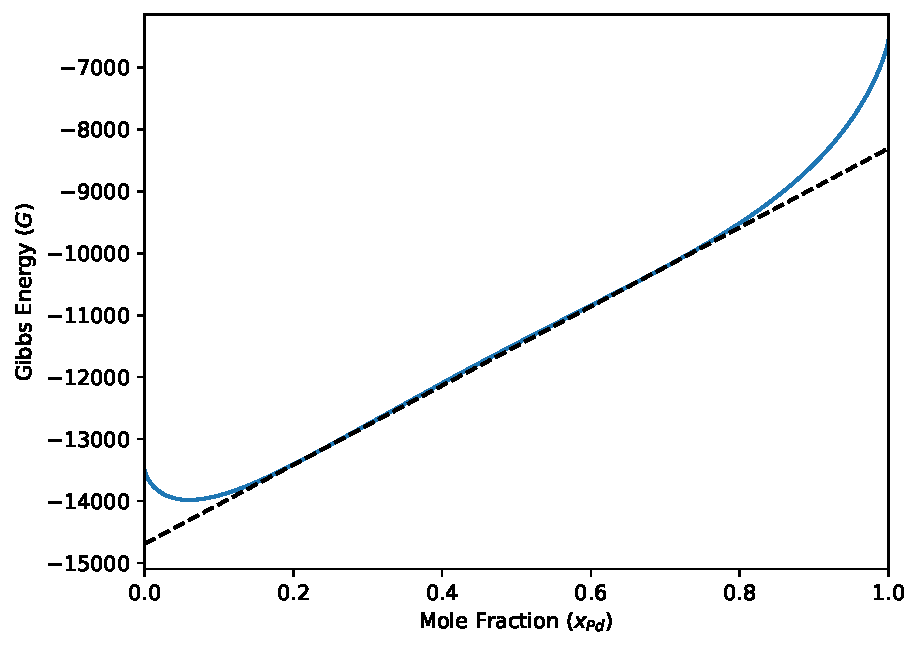
\includegraphics[width=0.675\textwidth]{figures/chapter-6/System_PdRh.pdf}
			\caption[Global optimisation test problem B: FCC phase miscibility gap in \ce{Pd-Rh} binary system.]{FCC phase miscibility gap in \ce{Pd-Rh} binary system from Kaye et al. \cite{Kaye07} shows a correctly identified miscibility gap which must be verified by the global optimisation algorithm.}
			\label{fig:testB}
		\end{figure}

	\item	\emph{Problem C}\\
		Another fictive binary system from Piro and Simunovic \cite{Piro16} with components \ce{C-D} can have three possible solution phases, the $\delta$ phase as shown in figure~\ref{fig:testC}. At  temperature  $T = 1100$ \si{\kelvin}, pressure $P=1$ \si{\atmosphere} and composition $x_{\ce{D}} = 0.6$, the $\delta$ phase is believed to be metastable but one must confirm that the combination of $\beta$ and $\gamma$ is most stable or if a different combination is more stable. However, it can be seen that inserting the $\delta$ phase into the system and replacing one of the other two phases would yield a lower value of the integral Gibbs energy of the system, $G_\text{sys}$. For this system, $g_{\ce{C}(\beta)}^\circ = 0$ \si{\joule \per \mole}, $g_{\ce{D}(\beta)}^\circ = 12471$ \si{\joule \per \mole}, $g_{\ce{C}(\gamma)}^\circ = 16628$ \si{\joule \per \mole}, $g_{\ce{D}(\gamma)}^\circ = 4157$ \si{\joule \per \mole}, $g_{\ce{C}(\delta)}^\circ = 26604$ \si{\joule \per \mole} and $g_{\ce{D}(\delta)}^\circ = 33256$ \si{\joule \per \mole}. The molar Gibbs energies of mixing are $g_{\beta}^\text{ex} = 41570 x_{\ce{C}} x_{\ce{D}} - 58198 x_{\ce{C}}x_{\ce{D}}^2$, $g_{\gamma}^\text{ex} = -5238 x_{\ce{C}} x_{\ce{D}}$ and $g_{\delta}^\text{ex} = -59445 x_{\ce{C}} x_{\ce{D}} - 74826 x_{\ce{C}}x_{\ce{D}}^2$.
		\begin{figure}[htbp]
			\centering
			\includegraphics[width=0.6\textwidth]{figures/chapter-6/System_CD.pdf}
			\caption[Global optimisation test problem C: Fictive system with three phases showing a false positive from thermodynamic equilibrium solver wherein a wrong phase is believed to be present at equilibrium.]{Fictive system with three phases showing a false positive from thermodynamic equilibrium solver wherein a wrong phase is believed to be present at equilibrium.}
			\label{fig:testC}
		\end{figure}
	
	\item	\emph{Problem D}\\
		Mixed oxide fuel (MOX) is a nuclear fuel that is manufactured by mixing plutonium dioxide recovered from used reactor fuel with depleted uranium dioxide and the \ce{Pu-U-O} ternary system from Gu\'{e}neau et al. \cite{Gueneau11} has been selected as a test problem. The thermodynamic assessment of the system contains an ideal gas, a non-ideal liquid,  and a \ce{(U_y Pu_{1-y})O$_{2\pm x}$} fluorite phase modelled using CEF with three sublattices and is an ionic phases where the first sublattice contains actinoid cations and the second and third sublattices contain oxygen anions mixing with vacancies. The global optimisation algorithm must respect the charge neutrality constraint thus distinguishing this problem from others. The system composition, as in \cite{Piro16}, is \SI{0.93}{\mole} of \ce{U}, \SI{0.07}{\mole} of \ce{Pu} and \SI{2}{\mole} of \ce{O} maintained at temperature $T = 1000$ \si{\kelvin} and hydrostatic pressure $P=1$ \si{\atmosphere}. The global optimisation algorithm must verify that the \ce{(U_y Pu_{1-y})O$_{2\pm x}$} fluorite phase is only stable phase at equilibrium.
		
	\item	\emph{Problem E}\\
		Otis et al. \cite{Otis:2017ab} demonstrated that  the \ce{Al-Co-Cr} ternary system modelled by Liu et al. \cite{Liu:2015aa} poses a challenge to thermodynamic equilibrium codes. In particular, it was shown that at temperature $T = 1523$  \si{\kelvin}, a ternary miscibility gap can be ignored when considering the metastable BCC phase only. The phase was modelled with a three-sublattice CEF model with the elements mixing on the first and second sublattices. Considering the challenges posed by the BCC phase in the system, the system was selected as a test problem with the system containing \SI{0.5}{\mole} of \ce{Al}, \SI{0.2}{\mole} of \ce{Co} and \SI{0.3}{\mole} of \ce{Cr} at $T = 1000$ \si{\kelvin} and $P=1$ \si{\atmosphere}. The global optimisation algorithm must identify the existence of a miscibility gap.
		\begin{figure}[htbp]
			\centering
			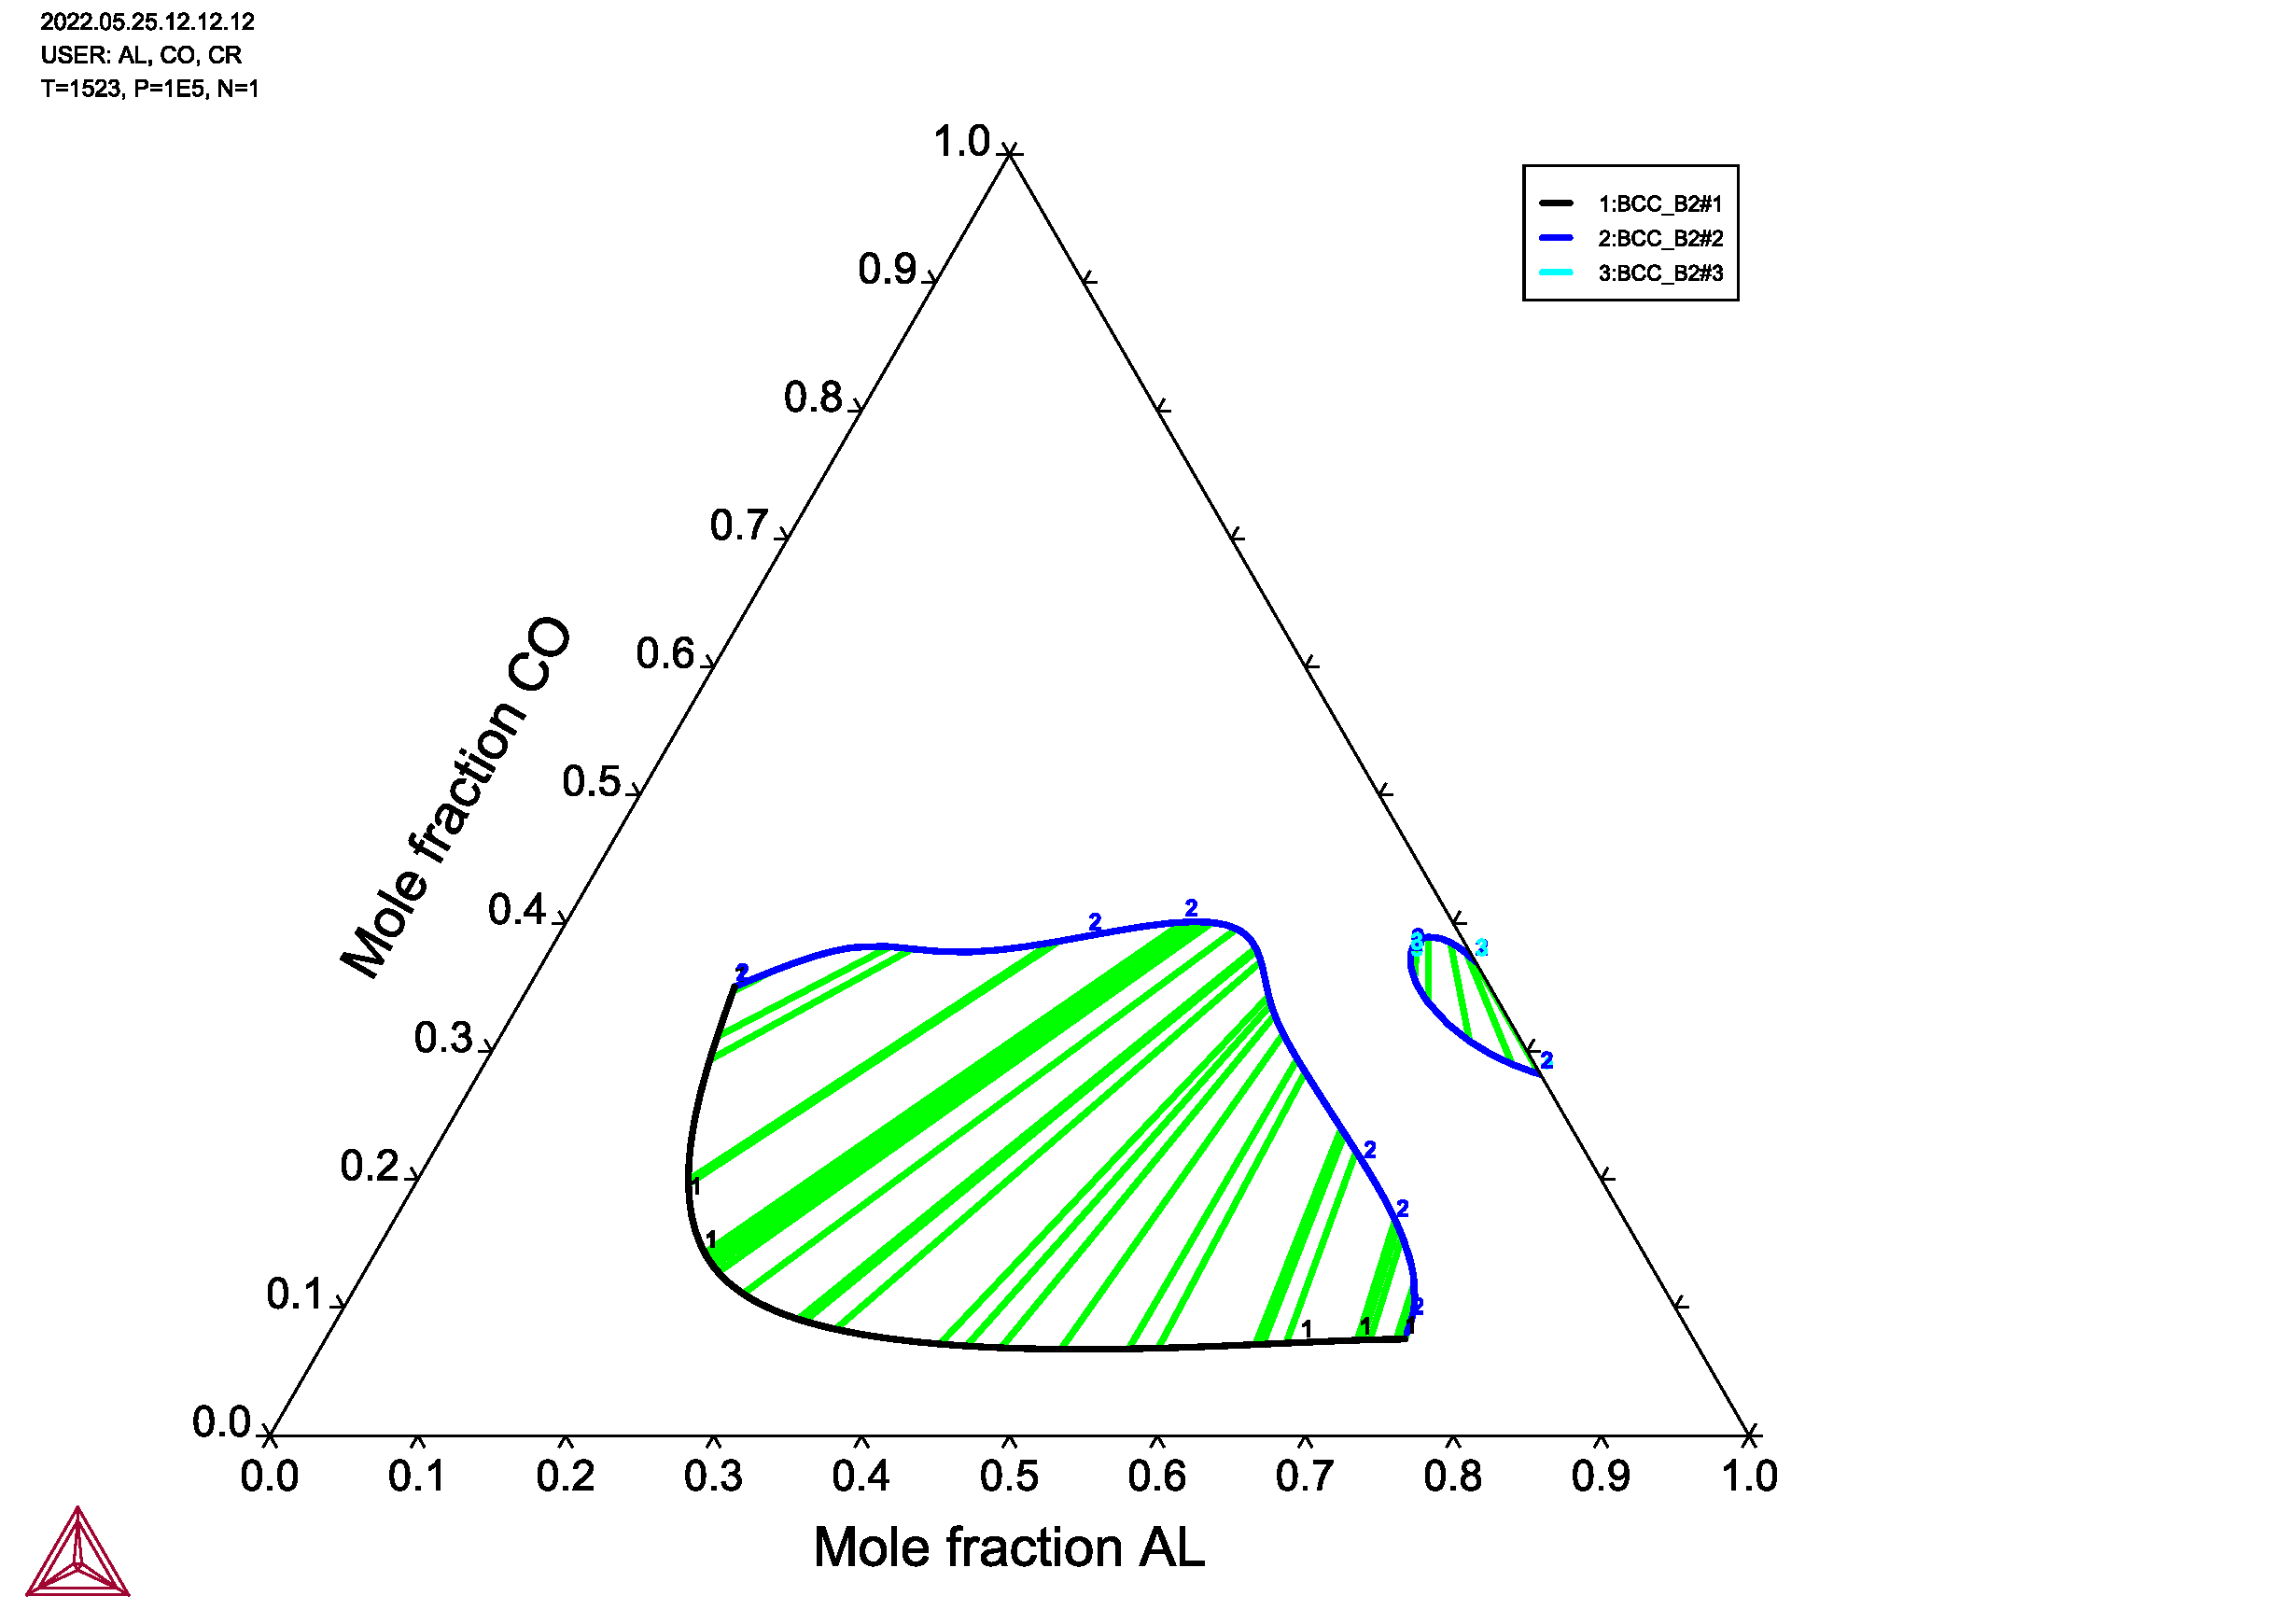
\includegraphics[width=0.6\textwidth]{figures/chapter-6/System_AlCoCr.pdf}
			\caption[Global optimisation test problem E: BCC phase \ce{Al-Co-Cr} ternary system with the miscibility gap.]{\ce{Al-Co-Cr} phase diagram calculated with Thermo-Calc version 2018b with an increased point density. With only BCC phase enabled, the existence of the miscibility gaps is shown in the central portion but as shown by Otis et al. \cite{Otis:2017ab}, the miscibility gap is lost using the default Thermo-Calc parameters.}
			\label{fig:testE}
		\end{figure} 
	
	\item	\emph{Problem F}\\
		The quinary \ce{Mo-Pd-Tc-Ru-Rh} system from Kaye \textit {et al.} \cite{Kaye07} is considered as the sixth test problem for comparing global optimisation algorithms. The system is relevant to nuclear reactor accident simulations as the components are noble metal fission products and their behaviour is critical to source term analyses. The system includes ideal gas, non-ideal liquid and four solid solution phases with face centred cubic (FCC), body centred cubic (BCC), hexagonal closed packed (HCP) and tetragonal crystal structures in addition to several stoichiometric phases. The liquid and solid solution phases were all modelled using substitutional solution models and, as in \cite{Piro16}, the system contains \SI{1}{\mole} of each component and is maintained at a temperature $T = 1000$ \si{\kelvin} and hydrostatic pressure $P=1$ \si{\atmosphere}. Examining the HCP phase only, the HCP--\ce{Mo9Pd11} phase combination is assumed to be stable and the global optimisation algorithms must identify the presence of a miscibility gap which yields a lower integral Gibbs energy of the system. The stable phase assemblage should be HCP--HCP miscibility gap co-existing with \ce{Mo9Pd11}.
	
	\item	\emph{Problems G \& H}\\
		The cases until now considered relatively simpler and smaller systems, which are easily visualisable and verifiable but a true representation of nuclear materials must consider a large number of system components. The last two test problems have been designed to test the global optimisation methods for a very large number of species. The fictive phases constructed for the high-dimensional tests are modelled using a three-sublattice CEF model with the first sublattice consisting of a large number of cations and the other two sublattices consisting of two anionic constituents mixing together. This results in two problems with 100 end members and 400 end members and is representative of irradiated molten salts. The fictive phases were constructed following the methodology of Piro and Simunovic \cite{Piro16}. The phases were assumed to have 10 and 30 components with 1-4 constituents per component. The cations were assigned a charge of +2 or +3 and the anions were assigned a charge of -1 (halides) or 0 (vacancy). The reference molar Gibbs energy of each end member was $g_i^\circ = \mathcal{U}(200, 450)$ \si{\kilo \joule \per \mole}. As in \cite{Piro16}, excess mixing parameters were created such that one cation would mix with the following cation in the list of constituents on the first sublattice with a mixing parameters ${^0}L = \mathcal{U}(-100000, 100000)$ and ${^1}L = \mathcal{U}(-1000, 1000)$.			
	\end{enumerate}

	\subsection{Grid sampling}
		Sampling from an equispaced grid has been widely adopted in thermodynamic equilibrium codes as a strategy for testing equilibria by performing numerous evaluations of the objective function at regular intervals in the domain \cite{Shobu09,Sundman85,Sundman15,Chen93a,Chen93b}. The method was developed in the 1970s and 1980s as a brute force method to verify global minimum for phase diagram construction problems and does not scale well for large systems. As shown in figure~\ref{fig:Grid_cons}, in the grid construction method, the surface of $\Delta G_\phi$ is discretised with each point treated as a stoichiometric compound and the ensemble of these compounds collectively approximates the driving force surface \cite{Piro16}. In the example figure, the arbitrary binary system consists of a solution phase and a stoichiometric phase and the domain for the solution phase has been sampled at nine equispaced grid points.
	\begin{figure}[htbp]
		\centering
		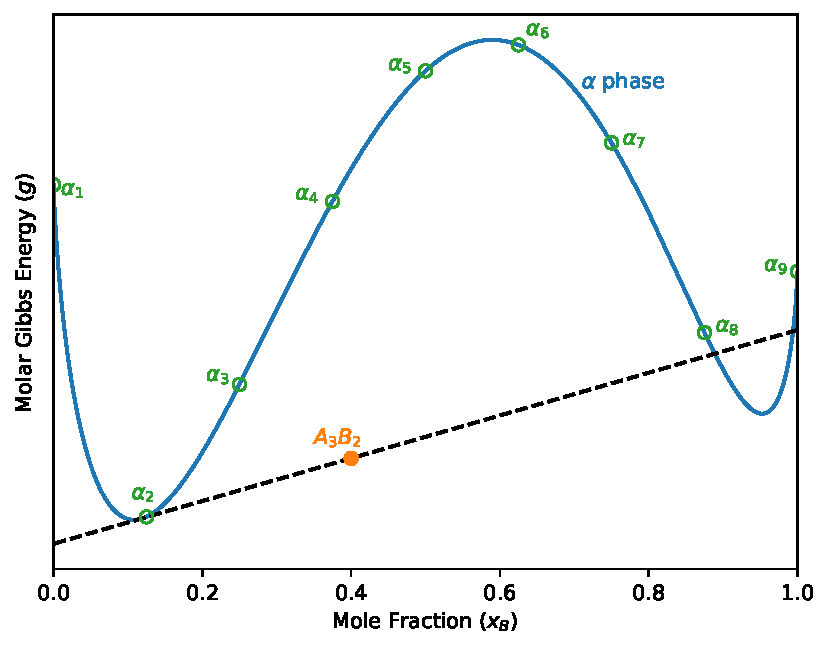
\includegraphics[width=0.65\textwidth]{figures/chapter-6/System_AB_grid.pdf}
		\caption{Demonstration of the grid construction method for fictive binary system in test problem A. The domain has been sampled at nine equispaced grid points and the pure stoichiometric phase \ce{A3B2} is found to be in equilibrium with the solution phase giving a false positive.}
		\label{fig:Grid_cons}
	\end{figure}

The discretisation of the grid plays a key role in the efficacy of this method and it has been shown by Chen et al. \cite{Chen93b} that the grid must be sufficiently resolved to avoid missing critical features such as the minimum between grid points $\alpha_8$ and $\alpha_9$ in figure~\ref{fig:Grid_cons}. However, this requirement leads to performance concerns as too small a grid leads to an increase in the computational cost while too large a grid can lead to false positives in the optimisation process.  Piro and Simunovic \cite{Piro16} have demonstrated how uniformly spaced grid for a phase $\phi$ in $N_\phi$ dimensional Euclidean phase (each dimension corresponds to a species in phase $\phi$) can result in an enormously large number of grid points depending on the grid size. In the example with nine grid points, it becomes clear from figure~\ref{fig:Grid_cons} that global minimum would not be found but increasing the number of grid points will lead to an exponential increase in the cost. In conclusion, the rapid increase in the computational cost with the reduction in grid size and a questionable performance in terms of reaching a global maximum tilts the scales against this method. Despite the fact, this method was tested with three separate grid spacings ($\delta = 0.1, \, 0.01, \,\text{and}\, 0.001$) to serve as benchmarks and to numerically show the rapid increase in computational time.
	
	\subsection{Spatial branch \& bound (sBB)}
		The Branch and Bound (BB or B\&B), attributed to Land and Doig \cite{Land:1960aa} who introduced it in 1960 for discrete programming, is a widely used algorithmic paradigm for finding optimal solutions to optimisation problems. As illustrated in \ref{fig:BB},the algorithm systematically enumerates all the candidate solutions by sequentially pruning out non-feasible solution candidates through a recursive approach of partitioning the domain and finding an upper and a lower bound for each subdomain. In 1969, Falk and Soland \cite{Falk69} proposed one of the first BB algorithms that could be applied to an continuous objective function with separable concave portions with a closed and convex set of constraints and a bounded feasibility region.
		\begin{figure}[htbp]
		\centering
		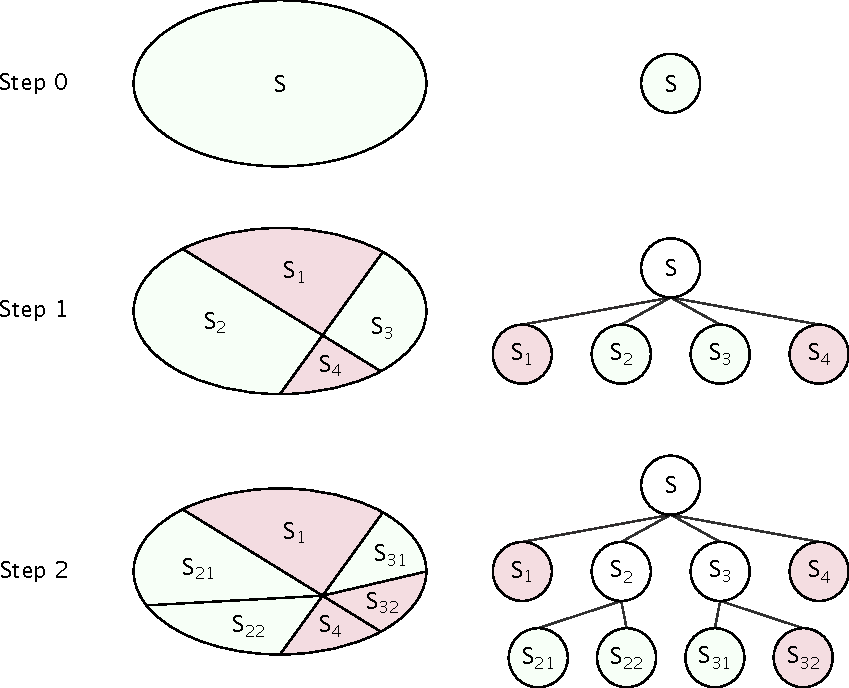
\includegraphics[width=0.65\textwidth]{figures/chapter-6/BB.pdf}
		\caption[Illustration of Branch and Bound (BB) class of algorithms.]{Illustration of the Branch and Bound (BB) class of algorithms. At each step, the domain is partitioned into a set of unexplored subdomains (denoted as nodes in a dynamic tree) which represent potential regions of optimal solution. By estimating the upper and lower bound on each subdomain, regions of infeasibility can be eliminated.}
		\label{fig:BB}
	\end{figure}
The BB algorithm involves two procedures to solve global optimisation problems:
	\begin{enumerate}
		\item \emph{Branching}: The domain $S$ is partitioned into two or more smaller disjoint domains $S_1,S_2,\dots,$ such that $S = S_1 \cup S_2 \cup \dots$ Thus, the partitioned objective function can be considered a convex approximation of the objective function within the subdomain $S_i$.
		\item \emph{Bounding}: The upper and lower bound of the objective function are found within a subset of the domain $S$. In the classical Branch and Bound method, a subdomain can be removed from the analysis if the lower bound of the objective function in it is greater than the upper bound of the objective function in any other subdomain.
	\end{enumerate}
McDonald and Floudas \cite{McDonald95} applied the BB algorithm to solve thermochemical equilibrium problems and Piro and Simunovic \cite{Piro16} proposed a modified version of the classical BB for the thermochemistry library {Thermochimica} which uses a different initialisation procedure and relaxation scheme for the bounds. Furthermore, instead of relying on pruning, every subdomain is evaluated till stopping criteria are met and if necessary, recursive partitioning technique is applied. The approach adopted by Piro and Simunovic \cite{Piro16} partitions the domain for each phase $\phi$ into $N_\phi$ subdomains and the driving force $\Delta G_\phi$ given by equation~\eqref{eq:DrivingForceLagrangian} is minimised in each subdomain. Their approach results in a Hessian which can be represented as a symmetric arrow matrix and by exploiting the structure of this matrix, the combination of $x_i$ that minimises $\Delta G_\phi$ can be easily determined. To solve the matrix, Gaussian elimination can be performed on the just the bottom row followed by back substitution. Furthermore, instead of storing a Hessian, the diagonal vector and a scalar representing the far right column can be stored. However, the implementation of this method warrants the use of an appropriate line search algorithm to ensure that the Wolfe conditions are satisfied and that the local system stays within the feasible region $0 < x_i <1$ . In addition, the step length must be suitably constrained to avoid missing any local minimums \cite{Piro16}. While the method works reasonably well, there are situations where it fails to correctly identify the true global minimum.

One of the best known method for solving non-convex nonlinear programming (NLP) problems is the \emph{spatial Branch and Bound (sBB)} \cite{Smith:1996aa,Tawarmalani:2013aa}. The branching, as already mentioned, is done by taking a continuous variable $v_i \in \left[v_i^l , v_i^u \right]$ and choosing $\beta \; (v_i^l \leq \beta \leq v_i^u)$ to create two subproblems with domains $\left[v_i^l , \beta \right]$ and $\left[\beta , v_i^u \right]$. When solving either subproblem, the original lower and upper bounds can be replaced by tighter bounds by taking the advantage of the reduced domain. This process, from McCormick \cite{McCormick:1976aa}, is called \emph{spatial branching}.
In this work, a \emph{Symbolic Reformulation sBB} \cite{Smith:1996aa,Smith:1997ab,Smith:1999aa} has been used through the Couenne (Convex Over and Under ENvelopes for Nonlinear Estimation) open-source software \cite{Belotti:2009aa,Belotti:2022aa}. Couenne has been developed to solve global optimisation problems $(\mathbf{P})$  of the form \cite{Belotti:2009aa}:
\begin{equation} \label{eq:couenne_prob}
\begin{aligned}
	\min \quad &f(x)			& \\
	\text{s.t.} \quad &g_j(x) \leq 0  	& &\forall j \in M \\
	&x_i^l \leq x_i \leq x_i^u	& &\forall i \in N_0 \\
	& x_i \in \mathbb{Z}		& &\forall i \in N_i^0 \subseteq N_0,
\end{aligned}
\end{equation}
where $f : \mathbb{R}^n \rightarrow \mathbb{R}$ and, $\forall j \in M$, $g_j : \mathbb{R}^n \rightarrow \mathbb{R}$ are multivariate functions, $n = \left|N_0\right|$ is the number of variables, and $x = (x_i)_{i \in N_0}$ is the n-vector variables. In the context of equilibrium thermodynamics, the problem in the form conformant to the above equation is as follows:
\begin{equation}
\begin{aligned}
	\min \; & \Delta G_\phi(x_i) = \sum_{i=0}^{N_\phi} \left( \tilde{\mu}_i - \sum_{j=1}^{C} \nu_{ij}\tilde{\Gamma}_j \right)		& \\
	\text{s.t.} \; &\sum_{i=1}^{N_\phi} x_i = 1  	& &\forall i \in N_\phi \\
			&\sum_{i=1}^{N_\phi} \nu_{i{e^-}} x_i = 0 & &\forall i \in N_\phi \\
	&0 \leq x_i \leq 1	& & \forall i \in N_\phi.
\end{aligned}
\end{equation}
Couenne implements linearisation, branching, heuristics and bound reduction and reformulates the problem by introducing a set of auxiliary variables. The reformulation of problem represented by equation~\eqref{eq:couenne_prob} results in the following form $(\mathbf{P'})$ \cite{Belotti:2009aa}: 
\begin{equation} \label{eq:couenne_reform}
\begin{aligned}
	\min \quad &x_{n+q}			& \\
	\text{s.t.} \quad &x_i = \vartheta_i \left(x \right)  	& &\forall i \in \{{n+1}, {n+2}, \dots, {n+q} \} \\
	&x_i^l \leq x_i \leq x_i^u	& &\forall i \in N \\
	& x_i \in \mathbb{Z}		& &\forall i \in N_i \subseteq N,
\end{aligned}
\end{equation}
where $N = \{{1}, {2}, \dots, {n+q} \}$ is the new variable index set which is a union of the original index set $\{{1}, {2}, \dots, {n} \}$ and the auxiliary index set $\{{n+1}, {n+2}, \dots, {n+q} \}$. $N_i$ denotes the index set of integer variables and the value of the last auxiliary variable, $x_{n+q}$, is the value of the objective function.

sBB algorithms rely on the generation of rigorous lower and upper bounds for the objective function value over any given variable subdomain. Generation of a upper bound is relatively simple as any feasible point of problem $(\mathbf{P})$ serves as an upper bound to the function at global minimum. In practice, it is best to chose the local minimiser of equation~\eqref{eq:couenne_prob} as the upper bound. When the reformulated problem $(\mathbf{P'})$ is in factorable form, the feature can be used to derive valid bounds and exact solution or one can use linear and quadratic approximations of $f$ and $g_j$. Detailed descriptions of sBB algorithms are found in literature \cite{Smith:1999aa,Liberti:2006aa} and the specifics to implementation in Couenne are described in \cite{Belotti:2009aa} but the method, illustrated in algorithm~\ref{alg:sBB}, is briefly described here. 
	
\SetKwComment{Comment}{/* }{ */}
\RestyleAlgo{ruled}
\begin{algorithm}[ht!]
	\caption[sBB algorithm for the MINLP problem $(\mathbf{P})$]{sBB algorithm for the MINLP problem $(\mathbf{P})$  \cite{Belotti:2009aa}.}
	\label{alg:sBB}
	\KwIn{Problem $(\mathbf{P})$}
	\BlankLine
	Define set $L$ of subproblems, $L \gets \{\mathbf{P}\}$\;
	Define upper bound $z^u$ for $\mathbf{P}$,  $z^u \gets \infty$\;
	\While{$L \neq \emptyset$}{
		Choose $\mathbf{P}_k \in L$\;
		$L \gets L \setminus \{\mathbf{P}_l\}$\;
		Apply bound tightening to $\mathbf{P}_k$\ \Comment*[r]{Bound tightening}
		\If{$\mathbf{P}_k$ is feasible after bound tightening}{
  			Generate a linear relaxation $\mathbf{LP}_k$ of $\mathbf{P}_k$\ \Comment*[r]{Linearisation}
    			\Repeat{$\bar{x}^k$ is feasible for  $\mathbf{P}_k$ or  $\bar{z}^k$ does not improve}{
				Solve $\mathbf{LP}_k$ to get an optimum $\bar{x}^k$ with objective value $\bar{z}^k$\;
				Refine linearisation  $\mathbf{LP}_k$\;}
			\If{$\bar{x}^k$ is feasible for  $\mathbf{P}_k$}{$z^u \gets \min{\{z^u, \bar{z}^k\}}$\;}
    			Find a local optimum $\hat{z}^k$ of $\mathbf{P}_k$\ \Comment*[r]{Upper bound calculation}
			$z^u \gets \min{\{z^u, \hat{z}^k\}}$\;
			\If{$\bar{z}^k \leq z^u - \epsilon$}{
			Choose a variable $x_i$\ \Comment*[r]{Branching variable selection}
			Choose a branching point $x_i^b$\ \Comment*[r]{Branching point selection}
			Create subproblems:\\
				$\quad\mathbf{P}_{k-}$ with $x_i \leq x_i^b$,\\
				$\quad\mathbf{P}_{k+}$ with $x_i \geq x_i^b$\;
			$L \gets L \cup \{\mathbf{P}_{k-}, \mathbf{P}_{k+}\}$\;				
			}
  		}
  	}
	\BlankLine
	\KwOut{$z_\text{out} \gets z^u$, an optimal solution of $(\mathbf{P})$}
\end{algorithm}
	
\begin{enumerate}
	\item \emph{Reformulation}\\
		A general method for allowing the formation of convex relaxation for any continuous twice differentiable function was given in \cite{Androulakis:1995aa,Adjiman:1996aa,Adjiman:1997aa} and a tighter relaxation framework was developed by Smith and Pantelides \cite{Smith:1999aa}. The goal of reformulation is to construct an equivalent formulation $\mathbf(P')$ to problem $\mathbf(P)$ such that it contains only linear constraints and special non-linear definitions. Since convex relations of many transcendental functions (such as logarithms, exponentials, etc.) exist and most algebraic expressions, including the ones encountered in equilibrium thermodynamics, are made up of binary operations of arithmetic and the unary operators, it is possible to construct convex relaxations of any algebraic expression. For doing this, additional variables can be introduced in the problem. For example, in test problem A, the non-linear terms in the excess mixing part can be reformulated as a linear problem by introducing variables $w_1 = x_A x_B$ and $w_2 = x_A x_B^2$. Such a process can be generalised and automated using the standard binary tree representation of algebraic expressions \cite{Smith:1996aa}. The reformulated problem $\mathbf(P')$ is equivalent to the original problem $\mathbf(P)$ but all the non-linearities are described by sets corresponding to bilinear product, linear fractional, simple exponentiation and univariate function terms. Because the two problems are equivalent, a convex relaxation of $\mathbf(P')$ is also a valid relaxation of $\mathbf(P)$. Hence, reformulation allows constructing a convex relaxation of any problem and the sBB determined optimal solution of $\mathbf(P')$ is also the optimal solution to $\mathbf(P)$.
	
	\item \emph{Linearisation}\\
		If one considers the constraint $x_j = \vartheta_j(x)$ created during reformulation and set $B = [x^l, x^u]$ defining bounds on the variables, a $\vartheta_j$-linearisation is a system of linear inequalities $A^j x \geq b^j$ such that $X_\text{LP} := {x \in B : A^j x \geq b^j} \supseteq {x \in B : x_j = \vartheta_j(x)}$. If a $\vartheta_j$-linearisation is created for each constraint $x_j$, a linear problem $\mathbf{LP}_k := \min{x_{n+q} : Ax \geq b}$ is a linear relaxation of $\mathbf{P}_k$ where $\mathbf{P}_k$ is a root node of $\mathbf{P}$ obtained through branching. The optimal solution $\bar{x}$ of $\mathbf{LP}_k$ provides a lower bound for the problem. If the solution of $\mathbf{LP}_k$ becomes infeasible for $\mathbf{P}_k$, the lower bound can be improved by either branching or refinement of $\mathbf{LP}_k$, i.e. by amending linearisation inequalities \cite{Belotti:2009aa}. Couenne uses a variant of the projection error rule for refinement \cite{Belotti:2009aa}.
		
	\item \emph{Bound tightening}\\
	According to Smith and Pantelides \cite{Smith:1999aa}, sBB can  achieve convergence without any bound tightening but the rate of convergence can be improved by using it. The goal of bound tightening is to reduce the interval $[x_i^l, x_i^u]$ without causing the optimal value of the problem to change and it allows reduction of the feasible set and an improved linearisation. One way of propagating the effects of constraints to variable bounds in Optimality-Based Bounds Tightening (OBBT) \cite{Liberti:2006aa,Quesada:1995aa,Smith:1996aa} but faster-feasibility bounds tightening (FBBT) are also available albeit resulting in weaker bounds \cite{Liberti:2006aa,Smith:1996aa,Shectman:1998aa,Sahinidis:2003aa}. In OBBT, two convex optimisation problems are solved:
	\begin{align}
		x_i^l = \min_x x_i, \quad \text{subject to convex relaxation constraints}, \quad x^l \leq x \leq x^u, \\
		x_i^u = \max_x x_i, \quad \text{subject to convex relaxation constraints}, \quad x^l \leq x \leq x^u.
	\end{align}
OBBT can be applied to every variable $x_i$ separately and when feasible the convex relaxation constraints can be updated but at each iteration it will solve $2N$ optimisation problems making it extremely expensive and suitable only for initial bound tightening steps \cite{Smith:1999aa}. FBBT, on the other hand, considers each constraint of the  reformulated problem individually \cite{Shectman:1998aa}. At any sBB node $k$, if the local minimum $\hat{x}^k \in \left[x^l, x^u\right]$ of the convex relaxed problem $\mathbf{CP}_k$ is known, FBBT is applied to fictitious bounding box $B \cap {x \in \mathbb{R}^{n+q} : x_i \leq \tilde{x}_i}$, where $\tilde{x}_i \in \left(x_i^l, \hat{x}_i^k\right)$ is suitably chosen. If the resulting problem become infeasible or if its lower bound becomes larger than the best upper bound, then $\left[\tilde{x}_i^k, x_i^u\right]$ is a valid tightening . On the other hand, if $\tilde{x}_i \in \left(\hat{x}_i^k, x_i^u\right)$ is chosen and FBBT applied to the analogous bounding box results in infeasibility, then $\left[x_i^l, \tilde{x}_i^k\right]$ is valid.
	
	\item \emph{Branching}\\
		Branching is critical to the performance of sBB and an effective strategy can help minimise the size of the sBB tree. The goal of branching is to choose a branch variable and corresponding branch point to be use to partition the domain. In doing so, the goal must be to improve the lower bound of the resulting subproblems and to eliminate as large an infeasible region as possible. In doing so, one must also try to keep the sBB balanced and together the three requirements are often conflicting and the implementations can be optimised to emphasise on one aspect or the other. Branching may be required when the lower bound $\bar{x}_{n+q}^k$ of an sBB node $\mathbf{P}_k$ is smaller than the best known feasible solution and the relaxation $\mathbf{LP}_k$ cannot be further refined. To objectively select the branching variable and point, Belotti et al. \cite{Belotti:2009aa} define the $\vartheta_i$-\textit{infeasibility} of auxiliary variable $x_i$ at node $k$ as $U_i\left(\bar{x}^k\right) = \left|\bar{x}_i^k - \vartheta_i\left(\bar{x}^k\right) \right| \slash \left(1 + \left \Vert \nabla \vartheta_i(\bar{x}^k)  \right \Vert_2\right)$. The scaling of the error term in numerator with the norm of the gradient avoids selecting a variable $x_i$ with a small bound interval $[x_i^l, x_i^u]$ but with a large $\left|\bar{x}_i^k - \vartheta_i\left(\bar{x}^k\right) \right|$ as it is unlikely to improve linearisation if used for branching.
		\begin{enumerate}
			\item	Branching variable selection\\
				In Couenne, integer variables have higher priority than continuous variable but since the driving force function results in a strictly NLP problem, continuous variables become the only candidate for branching. Defining the \emph{dependence set}, $D(x_i)$, as the set of variables in $\vartheta_i(x)$ (these are the variables in $x$ that $x_i$ directly depends on), the infeasibility of variable $x_i$ can be propagated to $D(x_i)$. In Couenne, Belotti et al. \cite{Belotti:2009aa} define the non-linear infeasibility as:
				\[
					\Omega_i^N(\bar{x}^k) = \mu_1 \sum_{j\in E(i)} U_j(\bar{x}^k) +  \mu_2 \max_{j\in E(i)} U_j(\bar{x}^k) +  \mu_3 \min_{j\in E(i)} U_j(\bar{x}^k),
				\]
				where for variable ${x}_i$, the set $E(i) = {j \in N \; : \; x_i \in D(x_j)}$. Parameter $\mu_k \geq 0, \, k = 1, 2, 3 $\footnote{Parameters $\mu_k$ defined here have no correlation to the chemical potential $\mu_i$.} and $\mu_1 + \mu_2 > 0$ ensures that $\bar{x}^k$ is infeasible if and only if $\Omega_i^N(\bar{x}^k) > 0$ for at least one variable $x_i$. In Couenne $(\mu_1, \mu_2, \mu_3) = (0.1, 1.3, 0.8)$ \cite{Belotti:2009aa}. The strategy, however, can often be ineffective and Couenne also has implementations of \emph{Violation Transfer} proposed by Tawarmalani and Sahinidis \cite{Tawarmalani:2004aa} and an extension of the \emph{reliability branching} technique introduced by Achterberg et al. \cite{Achterberg:2005aa}. In violation transfer, violations of non-convexities by the current solution are assigned to problem variables followed by transfer of violations to $D(x_i)$.  The. violations are then weighted to account for branching priorities and potential for convex relaxation improvement. The variable that leads to the maximum weighted violation is selected as the branching variable \cite{Tawarmalani:2004aa}. Since, the reliability branching strategy was not used in {\GEM}, a discussion of it is omitted and can be found in \cite{Belotti:2022aa}.
			\item Branching point selection\\
				For a continuous variable $x_i$ appearing in a single expression $x_j = \vartheta_j(x_i)$, the goal of sBB is to keep the resulting tree balanced. This makes areas of the linearisations a reasonable metric for selecting the branching point as shown in figure~\ref{fig:branching_pt}. In Couenne, three branching point selection strategies are implemented.
				\begin{figure}[htbp]
					\centering
					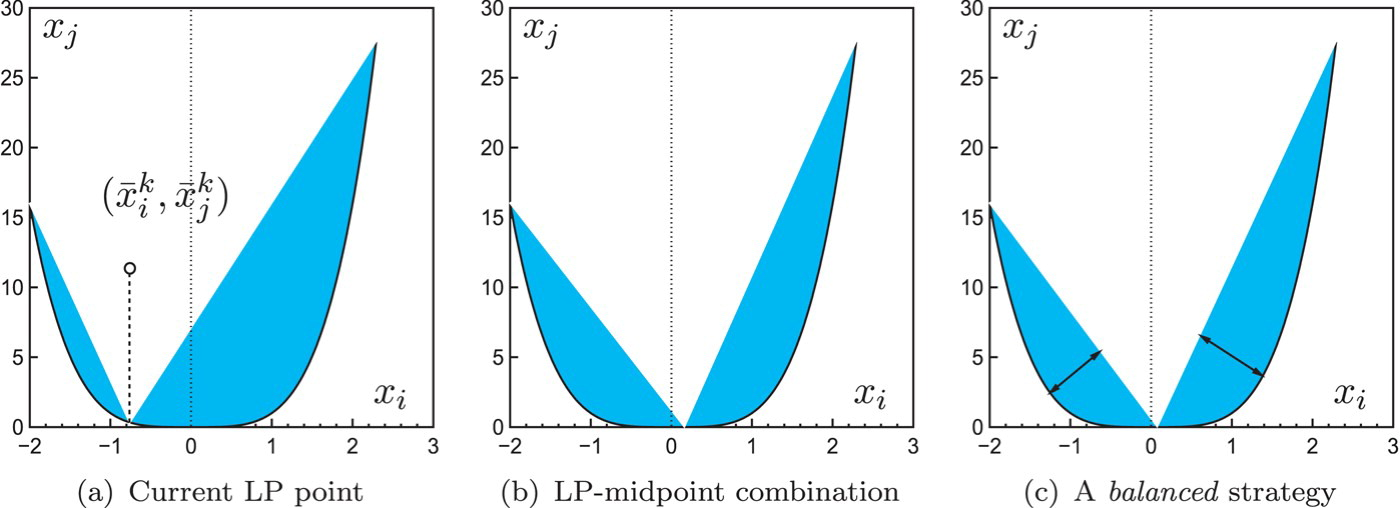
\includegraphics[width=\textwidth]{figures/chapter-6/branching_point}
					\caption[Strategies for selecting a branching point]{Strategies for selecting a branching point as implemented in Couenne: (a) branching on current LP solution $\bar{x}_i^k$, (b) Convex combination of LP point $\bar{x}_i^k$ and midpoint of bound interval, (c) Balancing the areas of the two resulting linearisations. Figure from Belotti et al. \cite{Belotti:2009aa}.}
			\label{fig:branching_pt}
			\end{figure}
		
		In the \emph{LP-based strategy}, the branching point is set so that $\bar{x}^k$ can become infeasible in both the subproblems. While simple to implement, as shown in subfigure (a) of figure~\ref{fig:branching_pt}, it can result in unbalanced subproblems. To avoid this, for variable $x_i \in [x_i^l, x_i^u]$, the branching point can be set as a convex combination of $\bar{x}_i^k$ and the midpoint of bound interval, $x_i^m = (x_i^l + x_i^u) / 2$ (see subfigure (b) of figure~\ref{fig:branching_pt}). Hence, a selection strategy guaranteeing a minimum distance from variable bounds is as follows \cite{Tawarmalani:2013aa}:
		\[
			x_i^b = \max \left \{x_i^l +b, \min \left \{x_i^u -b, \alpha \bar{x}_i^k + \left(1-\alpha\right)x_i^m \right \} \right \},
		\]
		where $0 < \alpha < 1$ and $b = \beta(x_i^u - x_i^l)$ for $0 < \beta < 0.5$ and $\alpha$ and $\beta$ are set to \num{0.25} and \num{0.2} respectively \cite{Belotti:2009aa} and  the strategy tries to balance the half-intervals of $x_i$. Alternatively, if a local minimum $\hat{x}^k$ is known, $\hat{x}_i^k$ can be chosen as a branching point since the resulting convexification will return a solution $\bar{x}^k$ that is very close to $\hat{x}^k$ \cite{Shectman:1998aa}.
		
	In \emph{expression-based strategies}, one can aim to reduce the sum of the areas of the resulting convexifications as shown in subfigure (c) of figure~\ref{fig:branching_pt}. Several methods for such strategy can be adopted \cite{Kalantari:1987aa,Liu:1996aa} but a balanced strategy implemented in Couenne finds the branching point using a binary search on the interval $[x_i^l, x_i^u]$ that minimises the difference between the maximum area $u'(x_i)$ and maximum area $u''(x_i)$ \cite{Belotti:2009aa}:
	\[
		x_i^b \in \argmin \left | \max_{x_i \in [x_i^l, x_i^b]} u'(x_i) - \max_{x_i \in [x_i^b, x_i^u]} u''(x_i) \right|,
	\]
	where $u'$ and $u''$ are the distance between the upper envelope line of $\vartheta_j$ and $(x_i, \vartheta_j(x_i))$ on the subdomains LP' and LP'' resulting from branching. The method balances the maximum distance between the points on $\vartheta_j(\cdot)$ and the upper envelope \cite{Belotti:2022aa}.
		\end{enumerate}	
\end{enumerate}

	  Together, the reformulation of the problem and the sBB algorithm result in a rigorous solution framework for global optimisation problem. Since the driving force functions are smooth and differentiable, they are well formulated for the method. Though the reformulation results in an increase in the size of the problem, it doesn't become a major issue for determining the minimum of the driving force.
	  
	
	\subsection{Particle swarm optimisation}
	
	Particle Swarm Optimisation (PSO) is a stochastic search algorithm inspired by the flocking behaviour of birds. First proposed by Kennedy and Eberhart \cite{Eberhart:1995aa,Kennedy95}, PSO is a population based method that relies on the premise of social sharing of information among a bird flock seeking food. PSO is relatively simple to describe and implement and its apparent competence in finding optimal solutions in complex search spaces has made it a widely studied search algorithm \cite{Freitas:2020aa}. In PSO, a population of candidate solutions, dubbed particles, moves around the search space as a function of the position and velocity of the particle and the movement of each particle is influenced by its best known local position and guided towards the best global position as other particles find better solutions. 

	At each iteration $t$, the velocity vector of particle $i$ in the swarm gets updated according to the following equation \cite{Bonyadi:2017aa}:
	\begin{equation} \label{eq:PSO_vel}
		\mathbf{v}_i^{t+1} = \omega \mathbf{v}_i^{t} + \psi_i {R_1}_i^t \left( \mathbf{p}_i^{t} - \mathbf{x}_i^{t} \right) +\psi_i {R_2}_i^t \left( \mathbf{g}^{t} - \mathbf{x}_i^{t} \right),
	\end{equation}
	where $\mathbf{v}_i^t$ and $\mathbf{x}_i^t$ are the velocity and position at iteration $t$. The inertia weight is given by $\omega$ and $\psi_1$ and $\psi_2$ are real acceleration coefficients known as cognitive weight and inertia weight respectively. Together, the weights control the impact of global and individual best positions on the particle's velocity and trajectory. Kennedy and Eberhart \cite{Kennedy95} originally assigned the same value of \num{2} to social and cognition parts but fine-tuning the parameters is critical to performance and convergence of PSO, particularly when dealing with multimodal problems \cite{Carlisle:2001aa,Trelea:2003aa,van-den-Bergh:2006aa}. $R_1$ and $R_2$ are uniformly distributed vectors used to maintain an adequate level of diversity in the swarm population and $\mathbf{p}_i^{t}$ and $\mathbf{g}^{t}$ represent the best known position of particle $i$ and the global best position of the swarm at iteration $t$. In turn, the position of each particle $i$ at every iteration $t$ can be updated according to the following equation \cite{Bonyadi:2017aa}:
	\begin{equation}  \label{eq:PSO_pos}
		\mathbf{x}_i^{t+1} = \mathbf{x}_i^{t} + \mathbf{v}_i^{t}.
	\end{equation}
	
	\SetKwComment{Comment}{/* }{ */}
\RestyleAlgo{ruled}
\begin{algorithm}[ht!]
	\caption[PSO algorithm for objective function $f : \mathbb{R}^n \rightarrow \mathbb{R}$]{PSO algorithm for objective function $f : \mathbb{R}^n \rightarrow \mathbb{R}$}
	\label{alg:PSO}
	\KwIn{Objective function $f$, Search space $\mathbf{x}_i = \left[\mathbf{x}_i^l, \mathbf{x}_i^u\right]$, Number of particles $N_p$}
	\BlankLine
	\For{Particle $i \in \{1, 2, \dots, N_p\}$}{
		Initialise initialise position, $\mathbf{x}_i \gets \mathcal{U}\left(\mathbf{x}_i^l, \mathbf{x}_i^u\right)$\;
		Initialise particle's best known position, $\mathbf{p}_i \gets \mathbf{x}_i$\;
		\If{$f(\mathbf{p}_i) < f(\mathbf{g})$}{
			Update global best position, $\mathbf{g}_i \gets \mathbf{p}_i$\;
		}
		Initialise the particle velocity, $\mathbf{v}_i \gets \mathcal{U}\left( - \left | \mathbf{x}_i^u - \mathbf{x}_i^l \right |, \left | \mathbf{x}_i^u - \mathbf{x}_i^l \right | \right)$\; 
	}
	\While{Termination criteria is not met}{
		\For{Particle $i \in \{1, 2, \dots, N_p\}$}{
			Pick random vectors, $\mathbf{R}_1, \mathbf{R}_2 \gets \mathcal{U}\left(0, 1\right)^n$\;
			Update particle velocity, $\mathbf{v}_i^{t+1} \gets \omega \mathbf{v}_i^{t} + \psi_i {R_1}_i^t \left( \mathbf{p}_i^{t} - \mathbf{x}_i^{t} \right) +\psi_i {R_2}_i^t \left( \mathbf{g}^{t} - \mathbf{x}_i^{t} \right)$\;
			Update particle position, $\mathbf{x}_i^{t+1} = \mathbf{x}_i^{t} + \mathbf{v}_i^{t}$\;
			\If{$f(\mathbf{x}_i^{t+1}) < f(\mathbf{p}_i) $}{
				Update particle's best known position, $\mathbf{p}_i^t \gets \mathbf{x}_i^{t+1}$\;
				\If{$f(\mathbf{p}_i^t) < f(\mathbf{g})$}{
				Update global best position, $\mathbf{g}^t \gets \mathbf{p}_i^t$\;
			}	
		}
	}
	}
	\BlankLine
	\KwOut{$x_\text{out} \gets \mathbf{g}^t$, an optimal solution of $f$}
\end{algorithm}

	The PSO algorithm, illustrated algorithm~\ref{alg:PSO}, has several advantages compared to other continuous optimisation methods. First, PSO is a problem independent algorithm, which only needs the objective function to evaluate the fitness of each candidate solution. In doing so, PSO does not make any assumptions about the continuity and differentiability of the objective function. Second, the evolution of particles is random and therefore the gradients of the objective function need not be calculated. Lastly, PSO does not need a good initial estimate or a-priori knowledge of the objective function search space \cite{Freitas:2020aa}. These factors have led PSO to gain a widespread appeal and it has shown good performance in several domains like function optimisation, artificial neural network training, fuzzy system control, etc. Unfortunately, for complex multimodal problems, the conventional PSO algorithm can get trapped in local optima, considerably compromising the convergence rate. This leads to poor performance and accuracy, and imposes restrictions on applicability to a wide range of practical problems \cite{Xu:2013aa,Harrison:2018aa}. While a-priori tuning can help improve performance, it is a time-intensive process but also assume that the optimal parameter configuration does not change over time. However, as shown by Leonard and Engelbrecht \cite{Leonard:2013aa}, the parameter values well-suited for exploration are not well-suited for exploitation and vice-versa. To achieve the two fold characteristic of good convergence speed and to avoid stagnating in local optima, several variations of PSO have been developed \cite{Shi:1998aa,Ratnaweera:2004aa,Chatterjee:2006aa,Fan:2007aa,van-den-Bergh:2001aa}. Another limitation of PSO is in constrained optimisation problem as it lacks an explicit constraint-handling mechanism. Several methods such as penalty function, feasibility-based rules method and the constraint-preserving method have been proposed with the penalty method being the most commonly used \cite{Sun:2011aa,Jordehi:2015aa}. While detailed discussions on handling these problems are available in open literature, the specific approach in the context of this work is discussed in the following text. 	
	
	\begin{enumerate}
		\item \emph{Constraint handling}\\
			As previously stated, several strategies have been explored to impose the constraints in PSO. One of the simplest constraint-handling mechanism is that of reseting the particles that escape the feasible region \cite{Hu:2002aa,Guo:2004aa,Sun:2009aa}. Minimisation of a non-stationary multi-stage assignment penalty function was proposed by Parsopoulos and Vrahatis \cite{Parsopoulos:2005aa} and the results were promising albeit at the cost of a very complex process for determining penalty. In the feasibility-based approaches such as that by Pulido and Coello \cite{Pulido:2004aa}, a candidate solution is chosen leader based on Deb's comparison rules \cite{Deb:2000aa}. The constraint handling strategy implemented in {\GEM} is based on the method by Hu and Eberhart et al. \cite{Hu:2002aa}. To make the solution more plausible, all the equality constraints are modified into inequality constraints to specified tolerance, i.e., the constraints on sum of mole fractions and the charge neutrality constraints are reformulated as:
			\begin{gather}
				\left | \sum_{i=1}^{N_\phi} x_i - 1 \right | <  \epsilon_1,\\
				\left | \sum_{i=1}^{N_\phi} \nu_{i{e^-}} x_i \right | < \epsilon_2.
			\end{gather} 
			The initialisation step is then modified to impose the constraints and once a feasible initial solution is found, the algorithm can progress. At every iteration $t$, each particle is checked for feasibility. If the updated position $x_i^{t+1}$ results in the bounds being violated, the step length is updated based on the following equation:
			\begin{equation}  \label{eq:PSO_pos_alpha}
				\mathbf{x}_i^{t+1} = \mathbf{x}_i^{t} + \alpha \mathbf{v}_i^{t},
			\end{equation}
			where $\alpha \in \mathcal{U} (0.1, 0.9)$ is a randomly generated constriction vector used to scale the step length. Handling the constraints, however is less straightforward. Once the position of each particle has been updated, the feasibility of each particle is verified and if it is found to violate the feasibility condition, Deb's comparison rules \cite{Deb:2000aa} are applied as follows:
			\begin{enumerate}
				\item	If all candidate solutions are infeasible, the candidate closest to feasibility is selected as the best candidate and the remaining particles are restored to previous feasible position. The best known position of these particles is not changed.
				\item If some candidates are feasible, their personal best is updated and the global best solution is selected from the feasible particles. The particles in infeasible regions are restored to the previous feasible solution.
				\item If all candidates are feasible, the same process as usual is followed.
			\end{enumerate}
			
		\item \emph{Particle initialisation}\\
			One of the parameters in PSO that can potentially affect the convergence rate is the number of particles and their initial positions. While the particle position $x_i$ is often initialised randomly from a uniform sampling in $\left[ x_i^l, x_i^u\right]$, it has been shown by Woronow \cite{Woronow:1993aa} that, when compared to normalised exponential distribution, normalised uniform distributions produce a poorer coverage of composition space. Otis et al. \cite{Otis:2017ab} employed a set of different sampling strategies such as Halton sequence, Sobol sequence and their variations to come come up with an efficient sampling strategy for PyCalphad. Furthermore, Piro and Simunovic \cite{Piro16} found that PSO often fails to capture the optimal solutions located close to the domain edges and special considerations must be taken when the optimal solution may exist close to the boundaries. To best see the effect of particles' initial position on the performance of PSO, a number of different options were tested. First, the number of particles, $N_p$, was selected from a finite set $\left\{ N_\phi, 2N_\phi\right\}$ and second, the particles were initialised using both normalised uniform and normalised exponential sampling. In addition, when $N_p = 2N_\phi$, a hybrid strategy was also used where $N_\phi$ particles were initialised using the sampling methods while the remaining $N_\phi$ particles were fixed at the corners of the domain. The reasoning behind this approach is that the particles closer to the edges should enable the spare closer to the edges to be properly explored. Also, more advanced sampling methods were not selected as, with well-tuned hyperparameters, PSO is expected to efficiently scan the domain unlike when only sampling is used and one must make sure that the features are not missed if the samples are not well picked. 

		\item \emph{Particle dynamics}\\
			Parameter tuning can have a significant impact on the performance of PSO and a large number of \emph{Adaptive PSO} (APSO) algorithms have been proposed in literature to overcome the problem of a-priori tuning of the parameters. A comparative analysis of many such algorithms has been performed by Harrison et al. \cite{Harrison:2018aa}. Amongst one of the promising APSO algorithms is \emph{APSO based on velocity information} (APSO-VI) proposed by Xu \cite{Xu:2013aa} which adapts the inertia weight based on the current velocity of the particles. The concept of APSO-VI is borrowed from Yasuda et al. \cite{Yasuda:2008aa} and aims to evolve the velocity to be close to an \emph{ideal} velocity. In APSO-VI the average velocity of swarm is defined as \cite{Xu:2013aa}:
			\begin{equation}
				\bar{v}^t = \frac{1}{n N_p} \sum_{i=1}^{N_p} \sum_{i=1}^{n} \left | v_{ij}^t \right |,
			\end{equation}
			where $n$ and $N_p$ represent the problem dimension and the number of particles in the swarm respectively. The size of the average velocity reflects the size of the particle search space and to better explore the search space, one should maintain a larger average velocity with longer time, during the early stage of the optimisation. On the other hand, during the latter stage, it is important to keep a small average velocity to find the optimum solution efficiently \cite{Xu:2013aa}. One can then define an ideal velocity at iteration $t$, which decreases with time, as follows:
			\begin{equation}
				{v}_\text{ideal}^t = v_s \left(\frac{1 + \cos\left (\frac{\pi t}{T_\text{end}} \right )}{2} \right),
			\end{equation}
			where $v_s = (x^u - x^l) / 2$ is the initial ideal velocity, $T$ is the maximum number of iterations and $T_\text{end} = 0.95 T$ is the time in which 95\% of search is completed. As visualised in figure~\ref{fig:APSO-ideal_v}, the ideal velocity profile matches the requirements for an effective exploration of the search space.
			\begin{figure}[htbp]
				\centering
				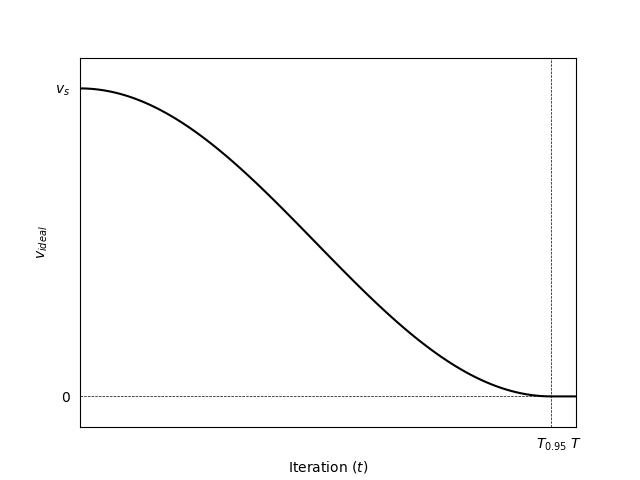
\includegraphics[width=0.75\textwidth]{figures/chapter-6/APSO-VI}
				\caption{Schematic of ideal velocity profile in APSO-VI.}
				\label{fig:APSO-ideal_v}
			\end{figure}
			The inertia weight can then be dynamically adapted at each iteration based on the average velocity in relation to the ideal velocity \cite{Harrison:2018aa} using:
			\begin{equation}
				\omega^{t+1} =  \begin{cases}
								\max \left\{ \omega^t - \Delta \omega, \, \omega_\text{min}\right\}& \text{if } \bar{v}^t \geq  {v}_\text{ideal}^{t+1}\\
								\min \left\{ \omega^t - \Delta \omega, \, \omega_\text{max}\right\}& \text{if } \bar{v}^t <  {v}_\text{ideal}^{t+1}
							\end{cases},
			\end{equation}
			where $\omega_\text{min}$ and $\omega_\text{max}$ are the minimum and maximum inertia weights and $\Delta \omega$ is the inertia weight step size. It has been shown by Harrison et al. \cite{Harrison:2016aa} that decreasing the ideal velocity decrease the inertia weight such that it remains within convergent range. Xu fixed the parameters $\omega_\text{min} = 0.3$, $\omega_\text{max} = 0.9$, $\Delta \omega = 0.1$, and $\psi_1 = \psi_2 = 1.49$ \cite{Xu:2013aa} and, in this work, APSO-VI has been adopted, albeit with slightly different parameter values. In {\GEM}, the APSO-VI hyperparameters were selected to be $\omega_\text{min} = 0.2$, $\omega_\text{max} = 0.9$, $\Delta \omega = 0.1$, $\psi_1 = 1.5$ and  $\psi_2 = 2$. These values provided good convergence rates while reasonably exploring the search space and are similar to those previously used in thermodynamic equilibrium application such as by Piro and Simunovic \cite{Piro16} and Myint et al. \cite{Myint:2021aa}.
	\end{enumerate}

	
	\subsection{Implementation and analysis}
	All global optimisation methods have their advantages and disadvantages and no global optimisation method is universally superior to others. While the deterministic methods are good at converging to a local minimum, they are often prone to high computational expenses. The stochastic methods, on the other hand, tend to cover the search space more effectively but face difficulty at finding the global minimum \cite{Piro16}. The global optimisation methods discussed in literature have mostly been problem centric and there has been a lack of a comprehensive and rigorous analysis of these methods applied to a variety of thermodynamic equilibrium problems. 	Since the global optimisation methods are critical to the performance of {\GEM}, an experimental approach was adopted to select method to be used. While the goal of the global minimiser can be restricted to identifying whether or not a phase has a negative driving force, in terms of comparison, the aim was to correctly identify the minimum of driving force in each of the eight test cases described in section~\ref{sec:test_global}.  
	
	Since, the convergence criteria for Couenne and the APSO-VI implementation differ, they must be clarified. In Couenne, the convergence is based on the feasibility tolerance. If a constraint $g_i(x) \leq 0$ within this tolerance, it is deemed satisfied \cite{Belotti:2022aa}. The Couenne solve requires several options to be specified. The ones of particular concern here were that related to branching for which violation transfer was selected and FBBT was applied to bound tightening. Since OBBT is computationally expensive, it was disabled and Couenne was allowed to use heuristics through interior point optimisation. The tolerance was left to the default value of ${10^{-6}}$.
	
	In APSO-VI, the convergence criterion is more complicated due to the stochastic nature of the algorithm. Guaranteeing that all the particles will converge to the same value is impossible without significantly compromising performance. Apart from a preset maximum number of iterations $T = 100$, the algorithm is deemed to converge if 95\% of the particles converge to a small distance of the global best position. For this, the Euclidean distance of each particle from the best known global solution is calculated using $S_i^t = \left \Vert x_i^t - g^t\right \Vert$ and if $S_i^t \leq 10-6$ for $0.95 N_p$ particles, the algorithm is terminated as converged. For calculating the Euclidean distance, only feasible solutions are considered and if a feasible global best is not identified, the algorithm is marked as failed.
	
	For comparison, each implementation of the method was executed a hundred times on a 2020 M1 MacBook Air with 8 GB of memory. The methods were alternated in ABC...ABC... pattern to avoid bias and the total time for all the runs was considered. The average time of all the times in the interquartile range was selected as the performance metric while the number of times the algorithm correctly identified the minimum or absence of negative driving force was the metric of reliability. No runs were discarded for the reliability metric. The results of a comparative analysis are shown in figures~\ref{fig:res_time} and \ref{fig:res_rel}. The results demonstrate that the equispaced grid sampling method is only effective with very small resolutions leading to a very rapid increase in the cost. On the other hand, the APSO is a lot more robust but they do show that a larger number of particles can better scan the space. Despite their efficiency, the robustness of the APSO is slightly lower than the sBB algorithm which converges to the correct results for each test case but does so at the cost of increase in computational time. 

\begin{figure}[ht!]
     \centering
     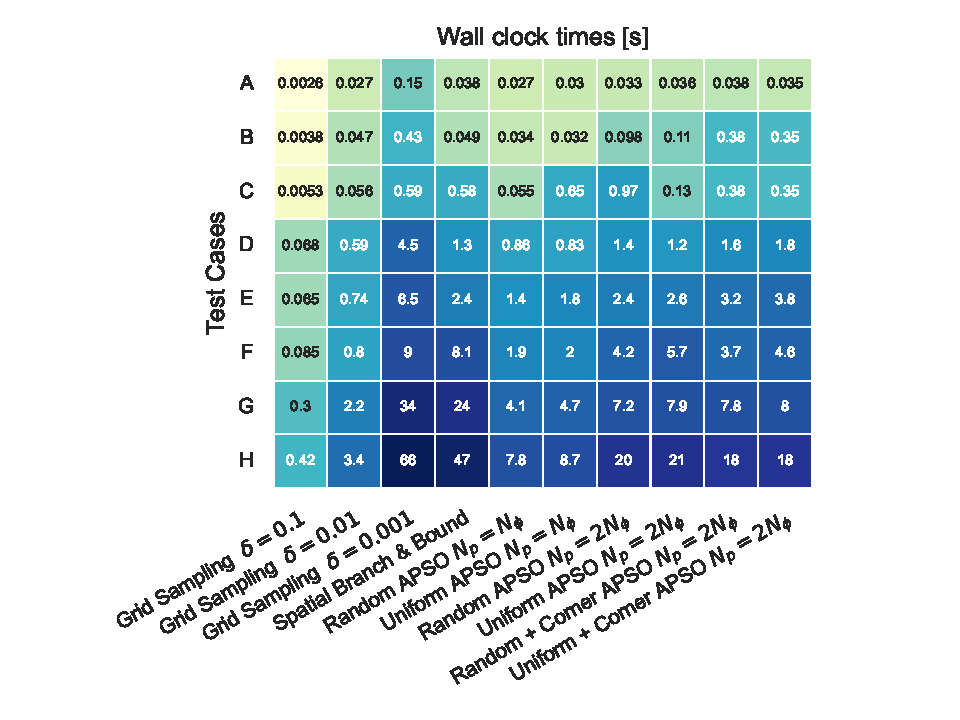
\includegraphics[width=0.9\textwidth]{figures/chapter-6/time.pdf}
     \caption[Comparison of computational performance of different global optimisation algorithms.]{Comparison of computational performance of various global optimisation algorithms for the test cases. The wall clock time is the average time of the results in interquartile range for 100 calculations of each method and case combination.}
     \label{fig:res_time}
 \end{figure}

\begin{figure}[ht!]
         \centering
         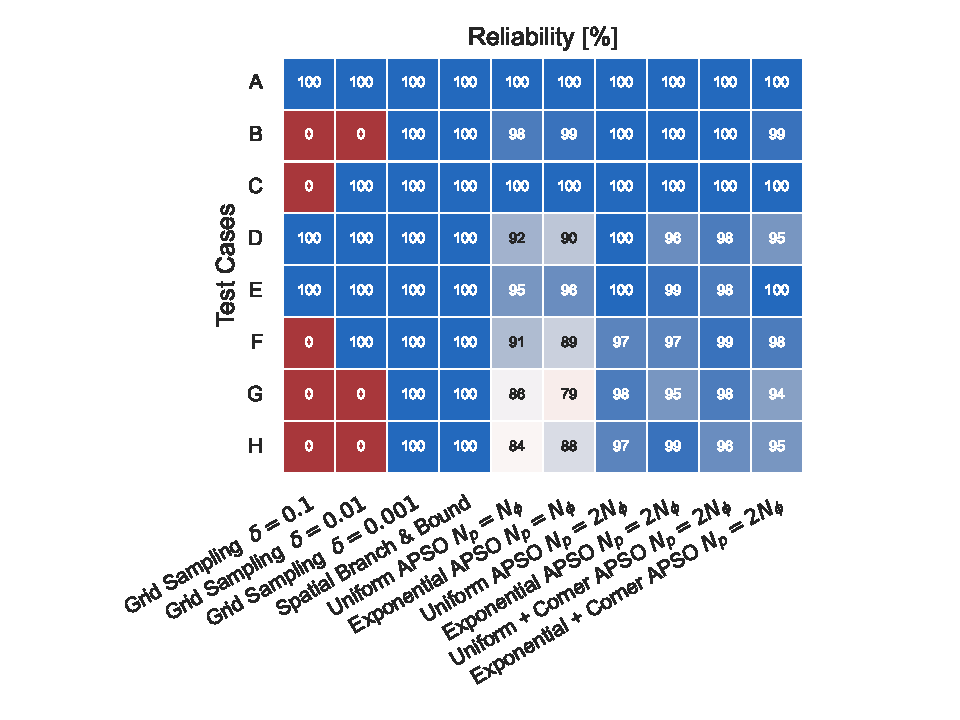
\includegraphics[width=0.9\textwidth]{figures/chapter-6/reliability.pdf}
     	\caption[Comparison of reliability of different global optimisation algorithms.]{Comparison of reliability of various global optimisation algorithms for the test cases. The reliability is the number of times the correct results were shown by a method out of the 100 calculations.}
	\label{fig:res_rel}
 \end{figure}
 
The grid sampling method was able to find the minimum in all the test cases albeit only when the grid resolution was increased to $\delta = 0.00$ and with a significant impediment on performance. In particular, one must be careful about the charge neutrality constraints with this approach. When dealing with ionic phases, many of the samples using this strategy will result in infeasibility due to the charge neutrality constraint getting violated. This can potentially compromise the method's reliability as a feasible point satisfying the charge constraint might never be found. In the implementation here, the objective function was evaluated at every sample point despite some of them being infeasible.

Among the tested options, sBB proves to be the most reliable though at a cost to performance. This is expected for the well behaved driving force functions. One way of reducing the computational cost of sBB is to terminate the solver as soon as an upper bound becomes negative or a feasible solution with negative driving force has been identified. This however has not been implemented in {\GEM}. The stochastic methods on the other hand exhibit fairly good computational performance though with a slightly lower reliability. In the experiments, the loss of reliability is attributable to reaching maximum iterations and in a small number of cases to converging to an infeasible value. Moreover, the impact of the number of particles in the swarm is clearly visible. With $N_p = N_\phi$, the space is not sufficiently scanned leading to a lower overall reliability. In such a scenario, increasing the number of particles seems to be the best choice but one must take cognisance of the fact that this can increase the computational time and might also require adjusting the convergence criteria. Initialising the particles on the corners did not have as big an impact as the number of particles. This can be attributed to the test cases itself where the optimal solution in most cases was not close to any edge and therefore no significant benefit was obtained from the particles scanning the space closer to the boundaries.

In the context of {\YJ}, both the sBB and APSO algorithms have been integrated into the code and the user will have the option of specifying the desired method. In cases where reliability is of the utmost and the system is deemed too complex, one could select sBB as the global optimisation algorithm while in cases where the system is deemed to be not very complicated or where there is a possibility of a-posteriori checking the results and / or augmenting global optimisation results with other information such as that from the grain information available in phase field.
	
\section{Software Quality Assurance (SQA)}
	A key thrust area of the {\GEM} development was to meet the SQA standards required from all MOOSE-based applications. Not only must one make sure that the results are physically representative, but the code itself must meet criteria for readability, uniformity and understandability but also avoid vulnerability and bugs.
{\GEM} has been developed following industry standard  development practices and procedures to ensure conformance to the MOOSE quality requirements. The key concepts worth mentioning are code review, source code control and continuous integration. MOOSE requires that any new code be reviewed by at least one reviewed other than the developer and the code can only be merged upon being approved. The main goal of the review process is to identify defects, improve code quality, finding better solutions to problems and ensuring coding guidelines are followed. The source code is maintained using the Git version control system and is hosted on INL's GitLab. Not only does it allow keeping a history of all the changes in the codebase but also enforces MOOSE syntax guidelines through Git hooks. MOOSE and hence {\GEM} use ClangFormat for all C++ code. {\GEM} also uses continuous integration (CI) using MOOSE's CI tool CIVET \cite{Slaughter:2021aa} and MOOSE's gold file based testing harness. Upon every commit to the repository, CIVET runs a suite of unit tests that verify the functionality of every separable code piece and also regression tests that test the whole code against known good results. Upon the completion of tests, a comprehensive report is generated that shows if the new code has breaks an existing functionality. The report also highlights the total and differential code coverage which is the percentage of code (lines and functions) that is hit in the tests. The last SQA process used in {\GEM} is code documentation. Every code is well documented through both in-code documentation and more detailed documentation pages that detail the different models, solvers and provide examples. Together, code review, version control, CI and documentation fulfil the SQA requirements of MOOSE-based applications.

\section{Summary}
	A number of algorithms for different parts of a thermodynamic equilibrium solver were presented in this chapter. Many of these algorithms have already been implemented in other codes available in the literature and GEM and levelling are well-matured algorithms. This is evident from the fact that most of the development efforts since the original GEM method have relied on auxiliary operations such as initialisation, etc. However, this does not mean that improvements can not be made.  The development of an advanced thermodynamic solver leaves the door open for incremental gains on many of these algorithms. The development of non-linear solver leverages state-of-the-art non-linear solvers available in PETSc and uses recent developments in algorithms for phase handling to minimise common pitfalls in many thermodynamic equilibrium codes. Finally, two of the major areas that stand to benefit from this work are global optimisation methods and integration with multiphysics framework {MOOSE}. The rigorous, experimental approach to global optimisation methods applicable to thermodynamic equilibrium provides measurable estimates for reliability, efficiency and robustness. The algorithms discussed here have been implemented in {\GEM} thus bringing native thermodynamic equilibrium capability to MOOSE.

\chapter{Conclusion}
\label{conclusion}

	Recent trends in modelling and simulation of various materials have adopted the multiscale approach wherein the information from smaller scales is used to develop and improve the models at larger scale in order to better simulate material behaviour. Nuclear materials, in particular, stand to benefit from these multiscale, multiphysics simulation models and have therefore driven the development of advanced modelling and simulation tools. The Multiphysics Object Oriented Programming Environment \texttt{(MOOSE)} developed by the Idaho national Laboratory enables such high fidelity simulations of nuclear materials and contains dedicated applications to model the behaviour of nuclear materials at various scales. However, it has, until now, lacked an application that can model corrosion at the meso-scale and efforts are now underway to develop a new application called \texttt{Yellowjacket}. An essential requirement of many nuclear material simulations is the ability to reliably predict the material properties as material composition evolves and it requires thermodynamic equilibrium calculations to predict the phase distribution at given temperatures and pressure. Particularly, for the case of corrosion modelling, the chemical potentials of various species that exist in the system acts as the driving force for corrosion. Therefore, there is considerable interest in integrating thermodynamic equilibrium computations in \texttt{MOOSE} and specifically \texttt{Yellowjacket}.
	
	The proposed research is aimed at developing a thermodynamic equilibrium solver to predict the phase assemblage of a multicomponent system for a given composition at isothermal, isobaric conditions. Through advanced algorithm development and efficient implementation of performance enhancing strategies, this research will focus on accelerating the performance of thermodynamic computations which are inherently very complex and can significantly impede the computational performance in coupled multiphysics codes. The need to minimise computation time while ensuring that the highly non-linear and non-convex system satisfies the conditions of thermodynamic equilibrium results in a challenging global optimisation problem. Over the course of this work, the Gibbs energy minimisation approach for computing thermodynamic equilibrium will be coupled with the proposed performance enhancing strategies and global optimisation schemes to efficiently and reliably predict the thermodynamic  equilibrium in large multicomponent systems. 
	
	The research will enable coupling thermodynamic equilibrium calculations within multiphysics codes and enable high fidelity material and process simulations to support the development of advanced nuclear reactors.
	
	
	
	
% \include{epilogue/epilogue}

\references{dissertation.bib}

%% Use letters for the chapter numbers of the appendices.
\appendix

%% Turn off thumb indices for unnumbered chapters.
\thumbfalse

% \include{cv/cv}
\chapter*{List of Publications}
\addcontentsline{toc}{chapter}{List of Publications}
\setheader{List of Publications}
\label{publications}

%% We use the 'etaremune' environment (the reverse of 'enumerate') to get a
%% numbered list of publications in reverse chronological order. If the list of
%% authors is long, it might be useful to emphasize your own name with \textbf.
\begin{enumerate}{\small
\item {M.\ Piro}, {M.\ Poschmann} and \textbf{P.\ Bajpai}, \textit{On the interpretation of chemical potentials computed from equilibrium thermodynamic codes: Applications to molten salts}, \href{https://doi.org/10.1016/j.jnucmat.2019.151756}{Journal of Nuclear Materials, 526 (2019) 151756}.
\item \textbf{P.\ Bajpai}, {M.\ Poschmann}, {M.\ Piro}, \textit{Derivations of useful partial molar excess Gibbs energy of mixing expressions of common thermodynamic models}, To be submitted to \href{https://www.journals.elsevier.com/calphad}{CALPHAD Computer Coupling of Phase Diagrams and Thermochemistry}. [In preparation]
\item \textbf{P.\ Bajpai}, {M.\ Poschmann}, {D.\ Andr\v{s}}, {C.\ Bhave}, {M.\ Tonks} and {M.\ Piro}, \textit{Development of a new thermochemistry solver for multiphysics simulations of nuclear materials}, \href{http://https://www.tms.org/TMS2020}{TMS 2020 Supplemental Proceedings, TMS 2020  - 149\textsuperscript{th} Annual Meeting \& Exhibition, San Diego, February 23-27, 2020}. [Accepted]
\item \textbf{P.\ Bajpai}, {M.\ Poschmann}, {D.\ Andr\v{s}} and {M.\ Piro}, \textit{Progress in developing a new thermochemistry code for corrosion modelling and multiphysics simulation of nuclear fuels}, \href{http://cns-annual-conference.org/2019/index.html}{39\textsuperscript{th} Annual Conference of the Canadian Nuclear Society and 43\textsuperscript{rd} Annual CNS/CNA Student Conference, Ottawa, June 23-26, 2019}.
}\end{enumerate}

\setboolean{@twoside}{false}

\newpage
\dedication{{M.\ Piro}, {M.\ Poschmann} and \textbf{P.\ Bajpai} \\ \textit{On the interpretation of chemical potentials computed from equilibrium thermodynamic codes: Applications to molten salts}\\ \href{https://doi.org/10.1016/j.jnucmat.2019.151756}{Journal of Nuclear Materials, 526 (2019) 151756}.}

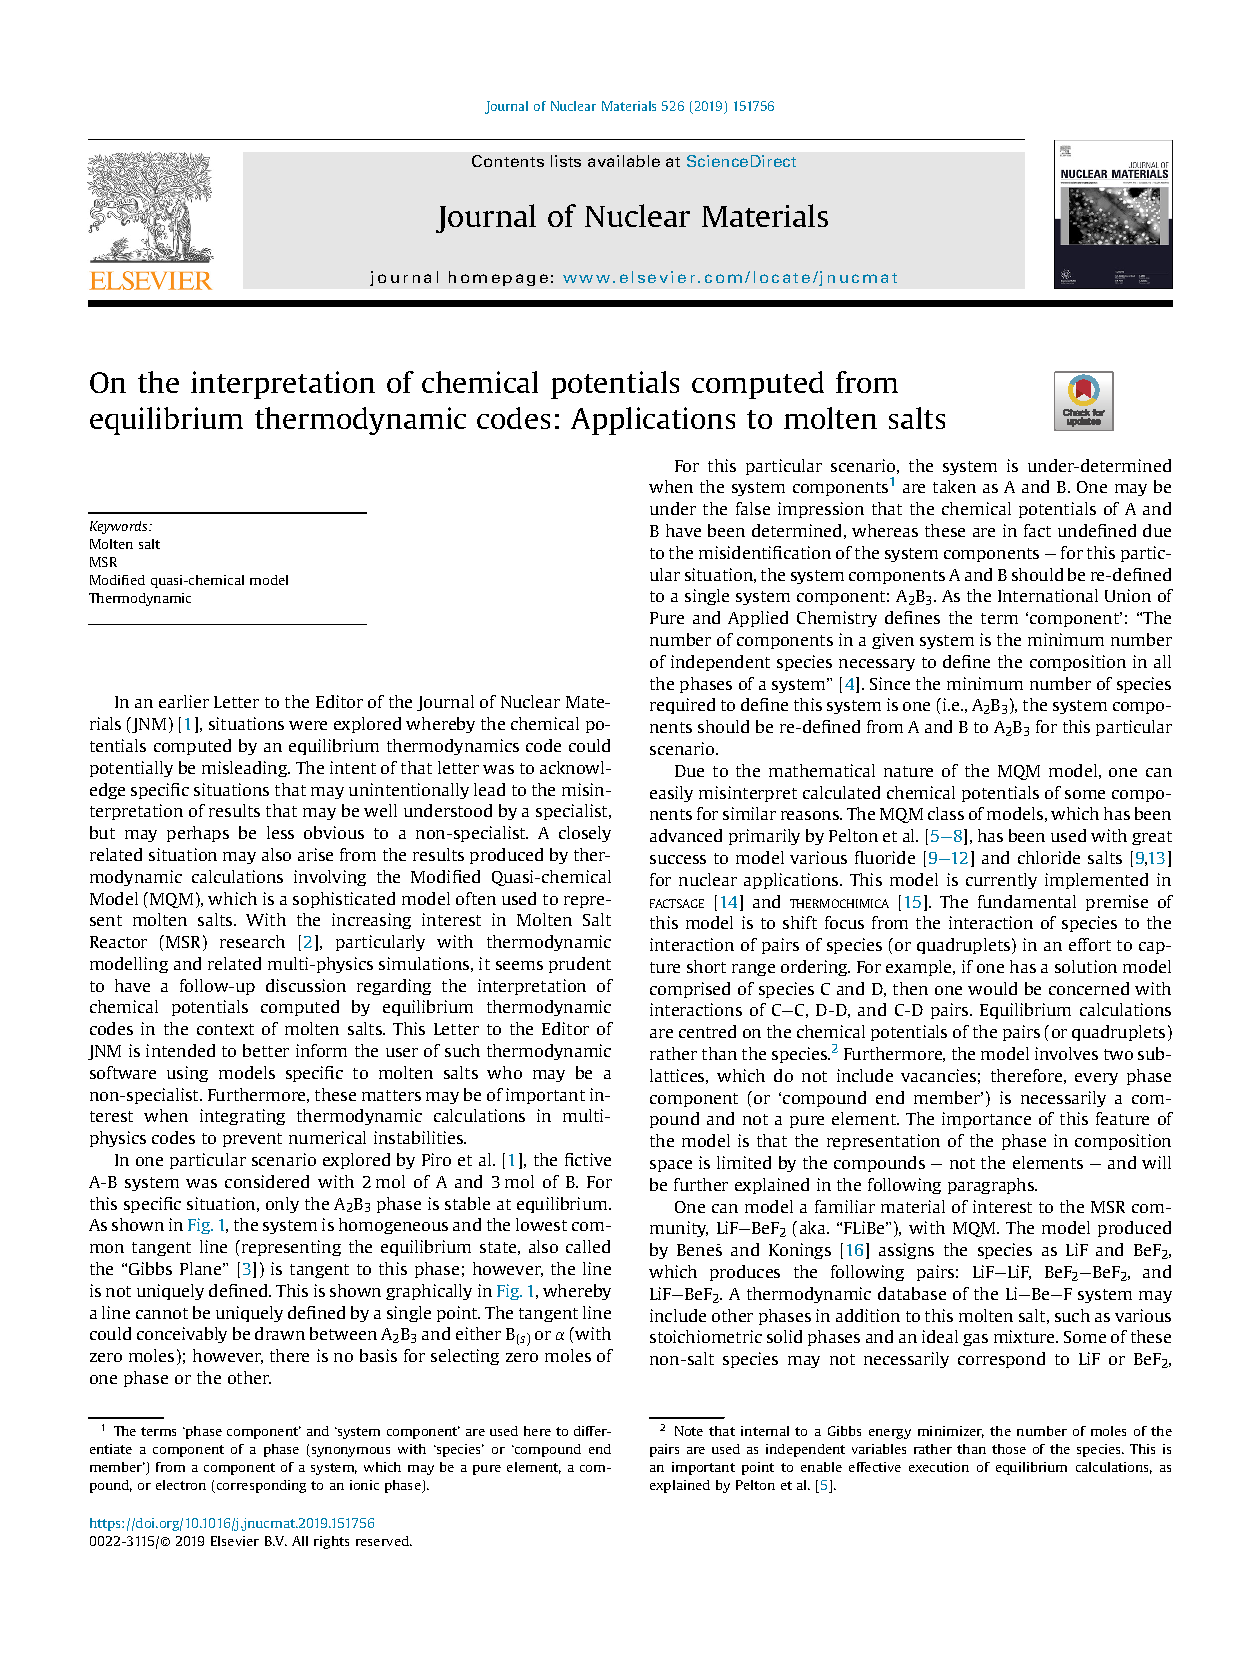
\includepdf[pages=-]{publications/Piro_JNM_2019.pdf}

\newpage
\dedication{\textbf{P.\ Bajpai}, {M.\ Poschmann} and {M.\ Piro}\\ \textit{erivations of useful partial molar excess Gibbs energy of mixing expressions of common thermodynamic models}\\ To be submitted to \href{https://www.journals.elsevier.com/calphad}{CALPHAD Computer Coupling of Phase Diagrams and Thermochemistry}. [In preparation]}

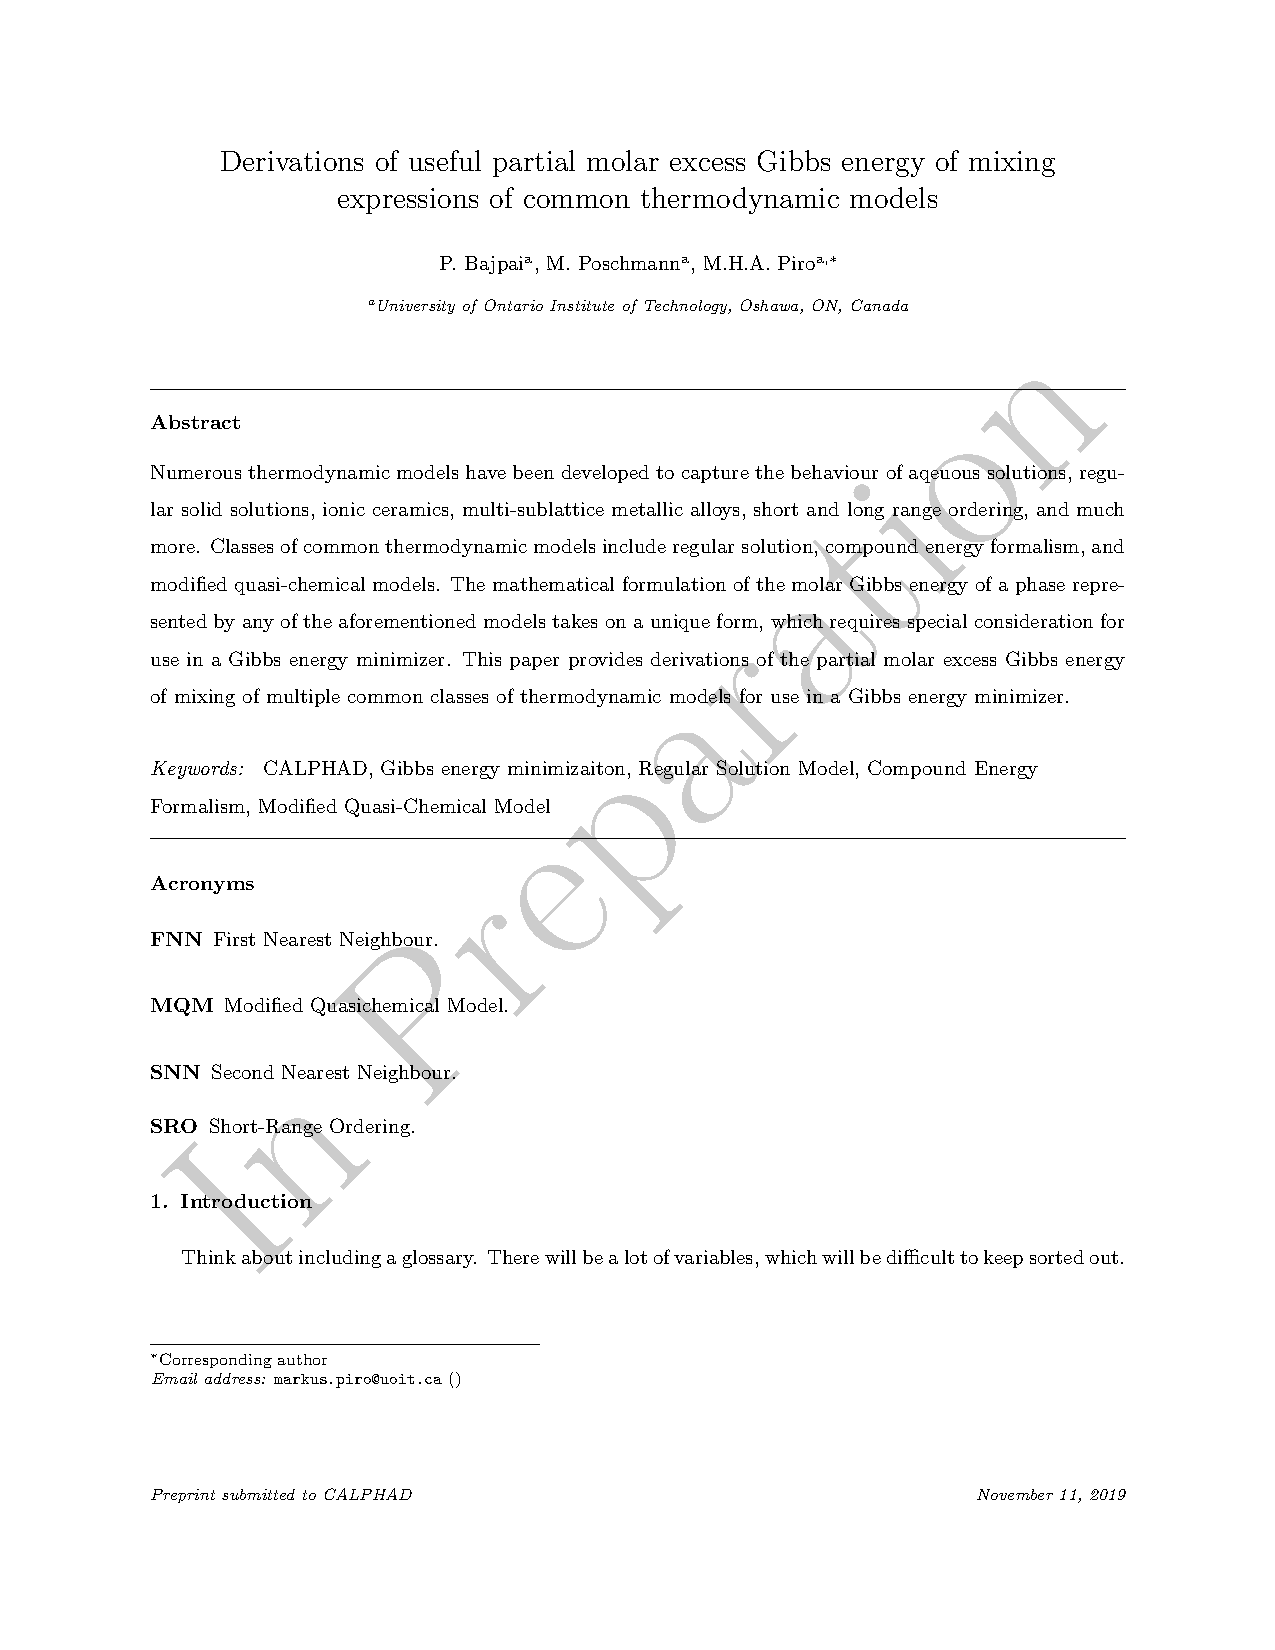
\includepdf[pages=-]{publications/Bajpai_Calphad_2020.pdf}

\newpage
\dedication{\textbf{P.\ Bajpai}, {M.\ Poschmann}, {D.\ Andr\v{s}}, {C.\ Bhave}, {M.\ Tonks} and {M.\ Piro}\\ \textit{Development of a new thermochemistry solver for multiphysics simulations of nuclear materials}\\ \href{http://https://www.tms.org/TMS2020}{TMS 2020 Supplemental Proceedings, TMS 2020  - 149\textsuperscript{th} Annual Meeting \& Exhibition, San Diego, February 23-27, 2020}. [Accepted]}
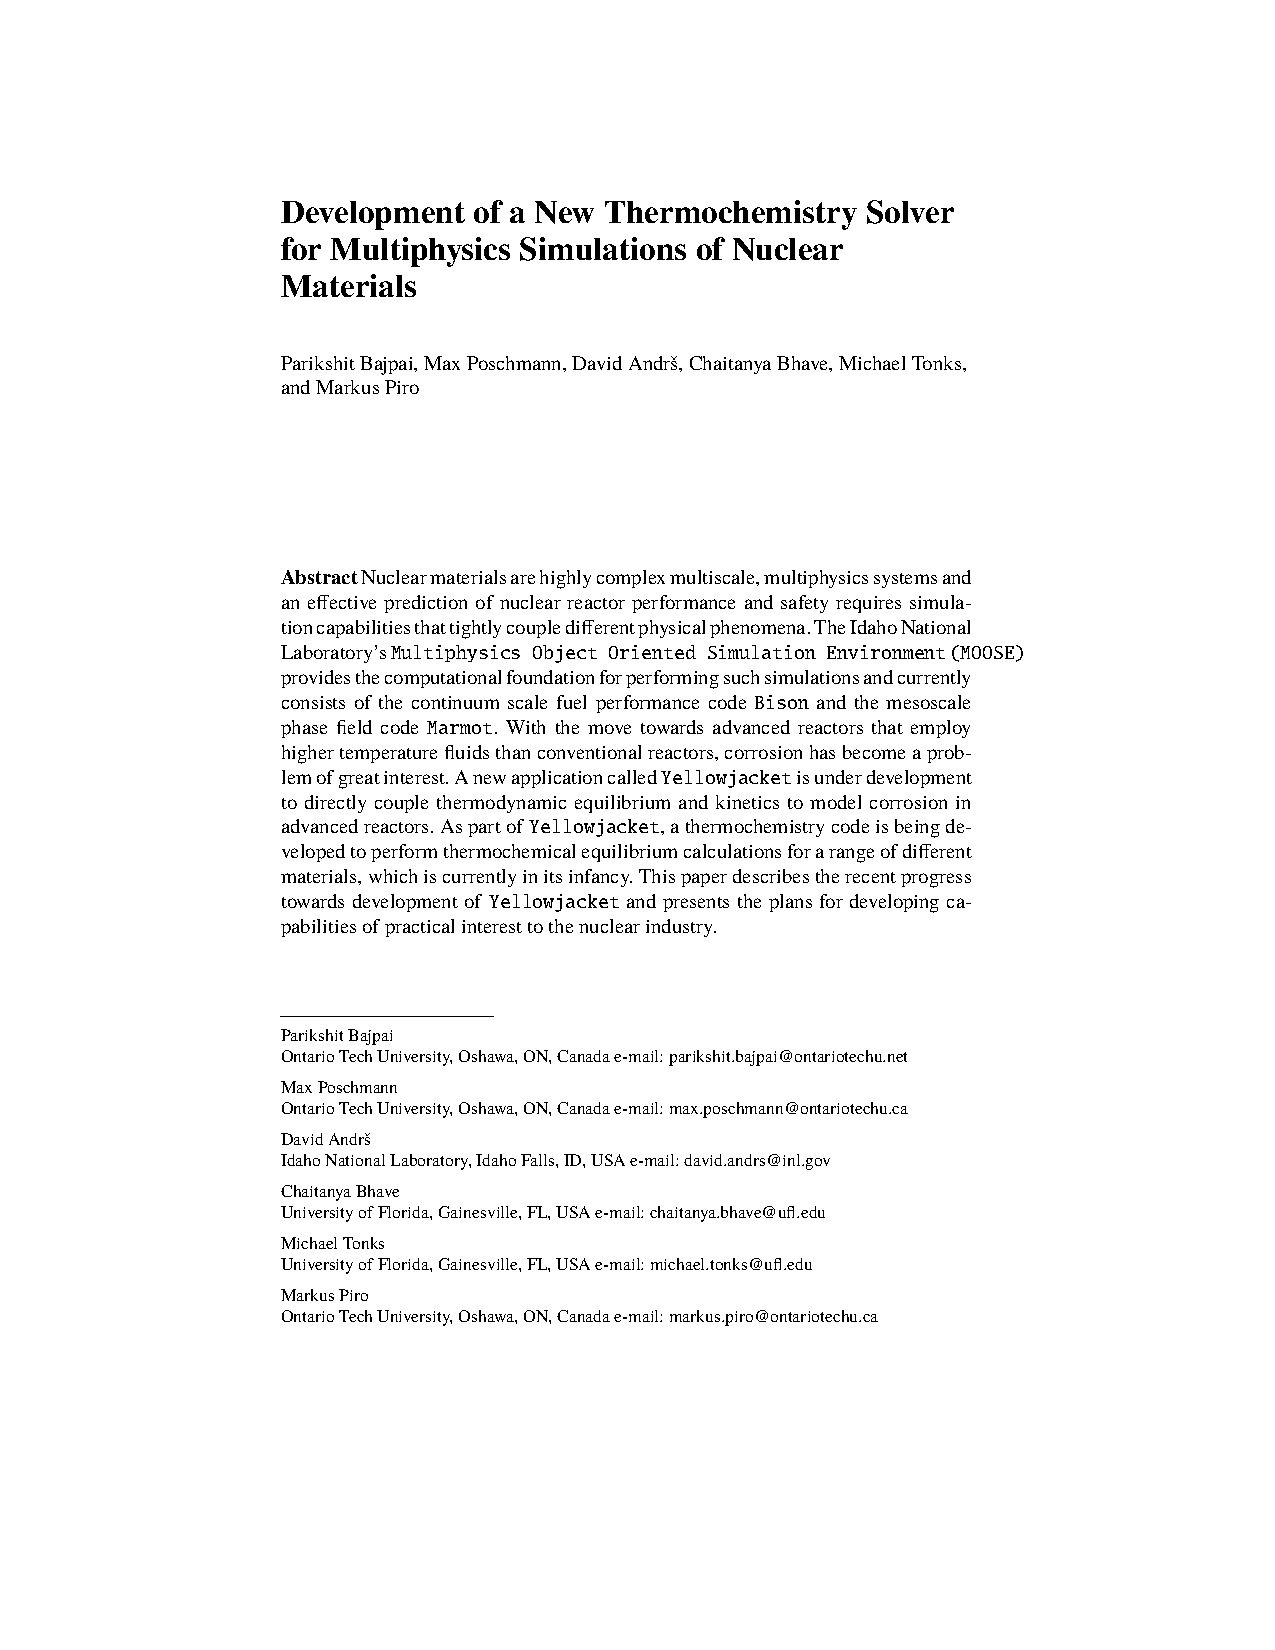
\includepdf[pages=-]{publications/Bajpai_TMS_2020.pdf}


\setboolean{@twoside}{false}

\newpage
\dedication{
\textbf{P.\ Bajpai}, {M.\ Poschmann}, {D.\ Andr\v{s}} and {M.\ Piro}\\ \textit{Progress in developing a new thermochemistry code for corrosion modelling and multiphysics simulation of nuclear fuels}\\ \href{http://cns-annual-conference.org/2019/index.html}{39\textsuperscript{th} Annual Conference of the Canadian Nuclear Society and 43\textsuperscript{rd} Annual CNS/CNA Student Conference, Ottawa, June 23-26, 2019}.}
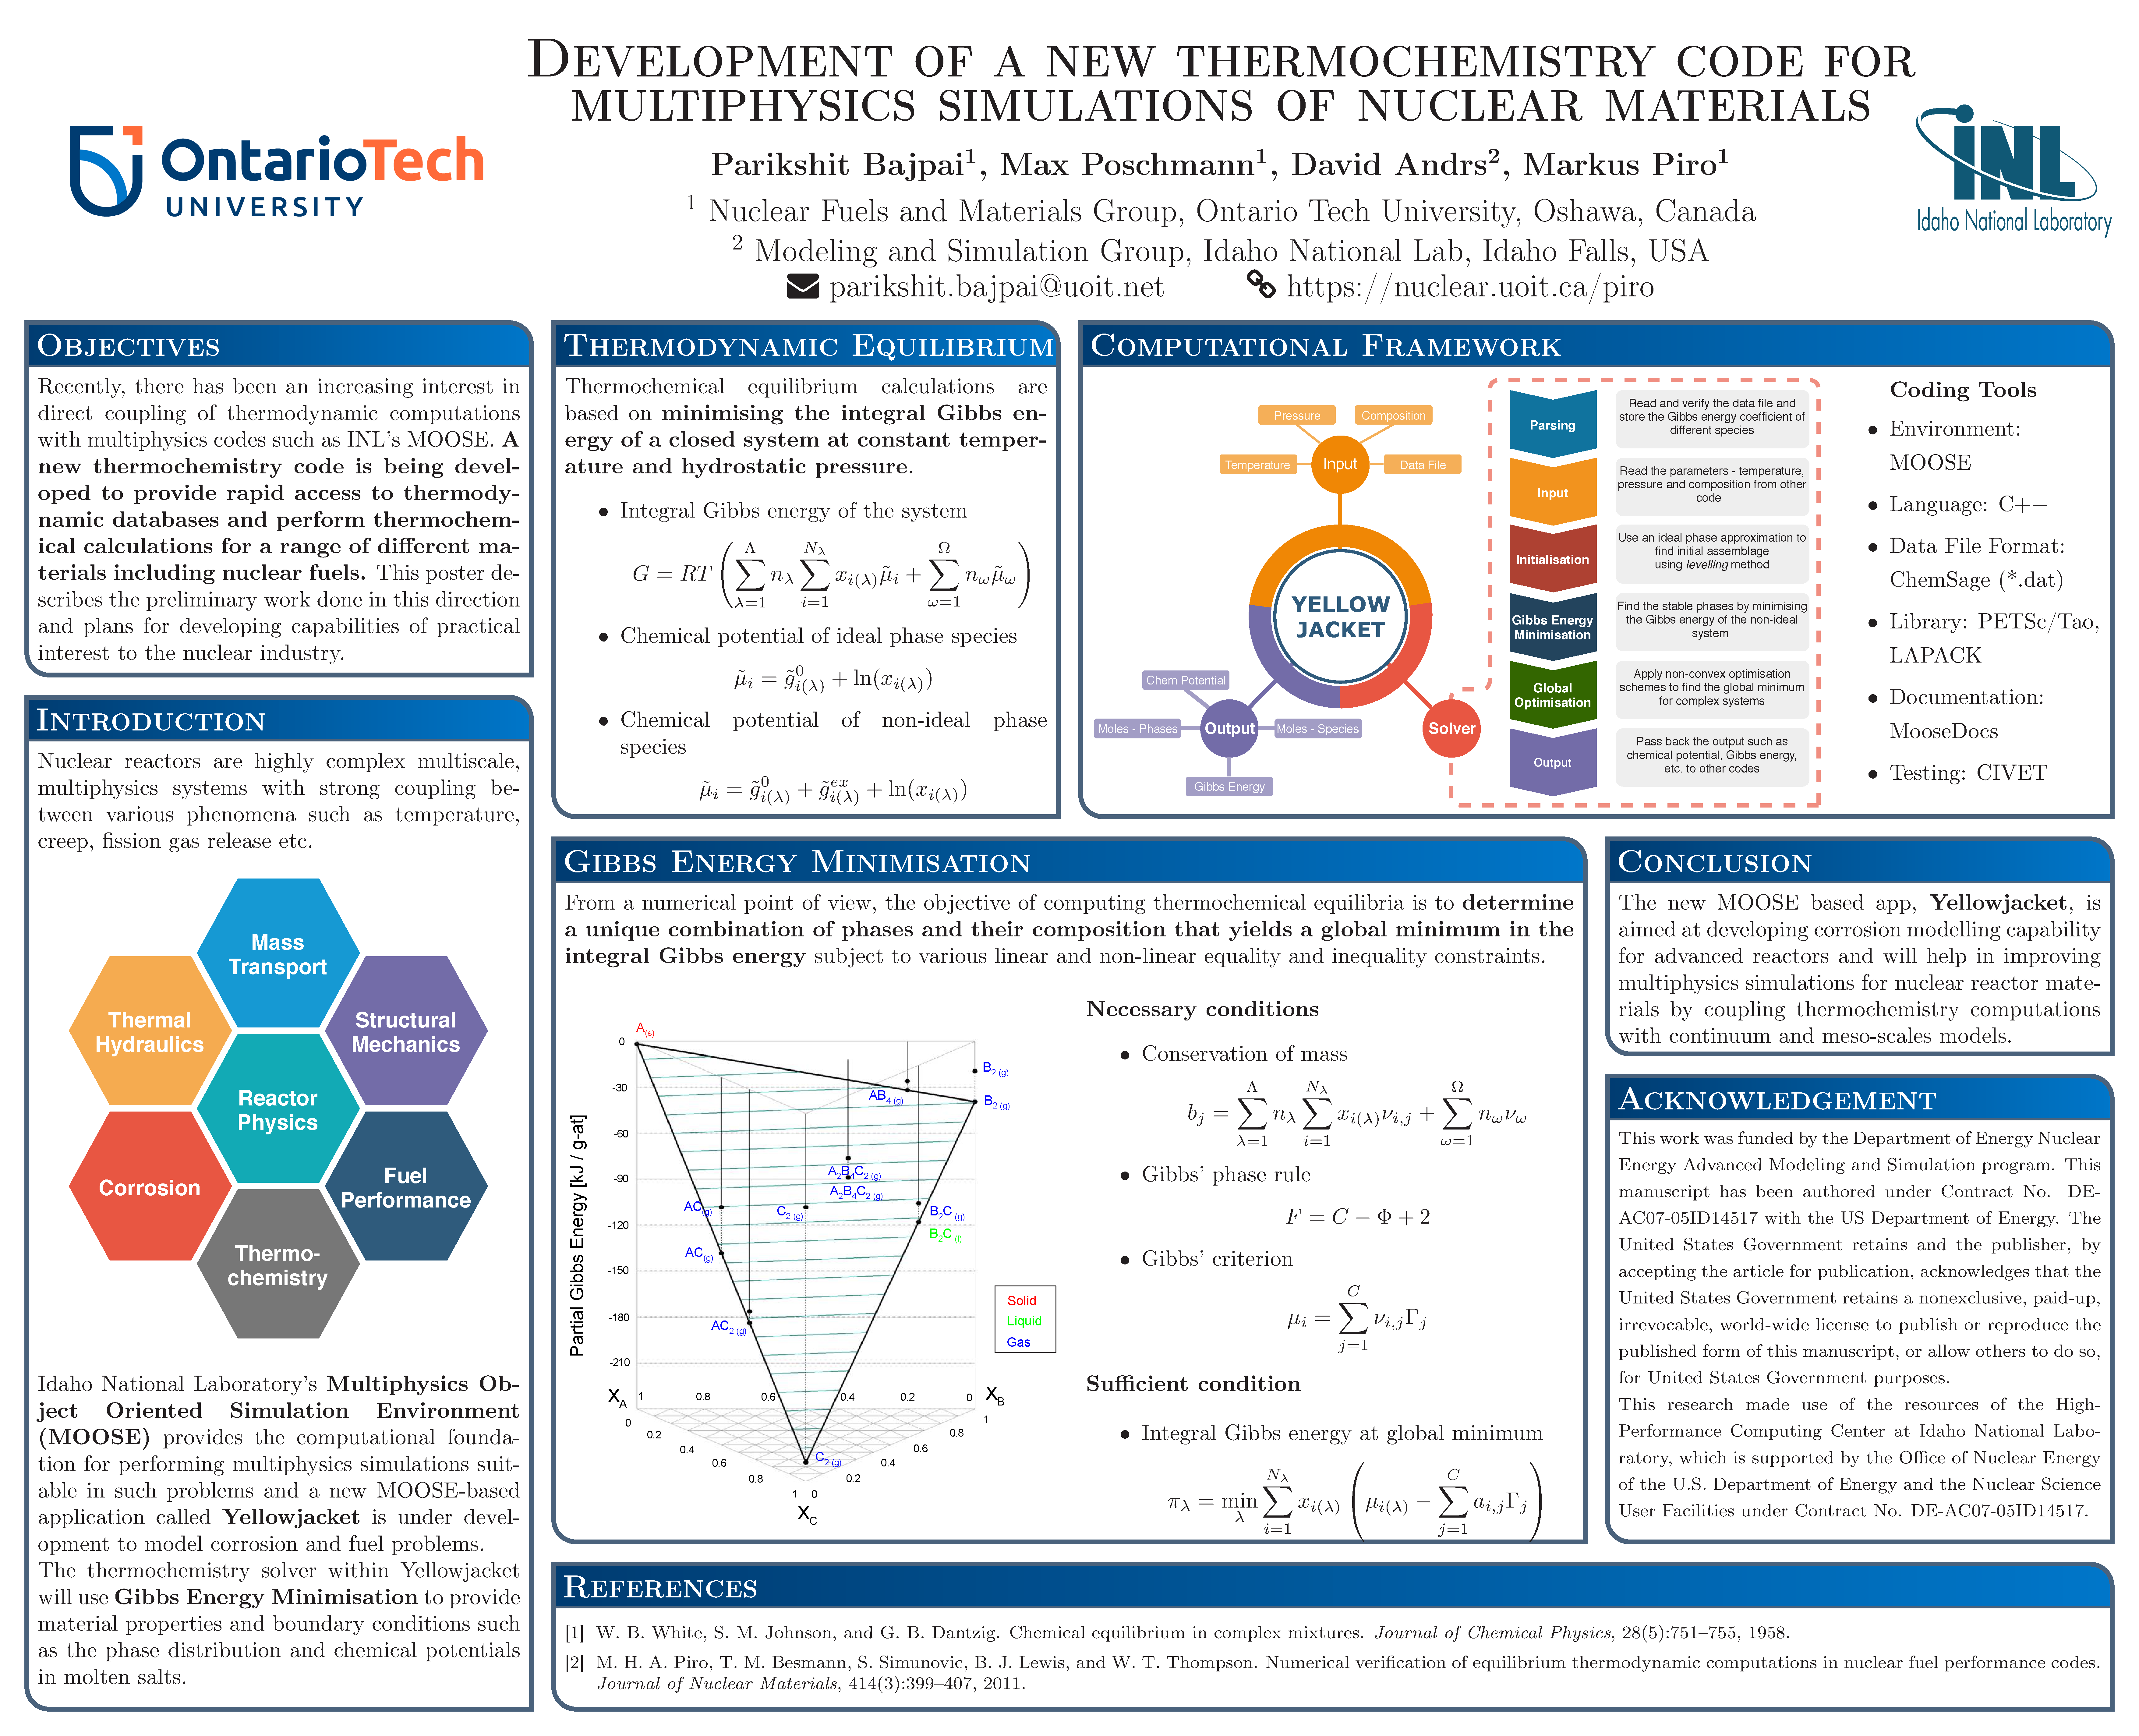
\includepdf[pages=-]{publications/CNS_Poster.pdf}
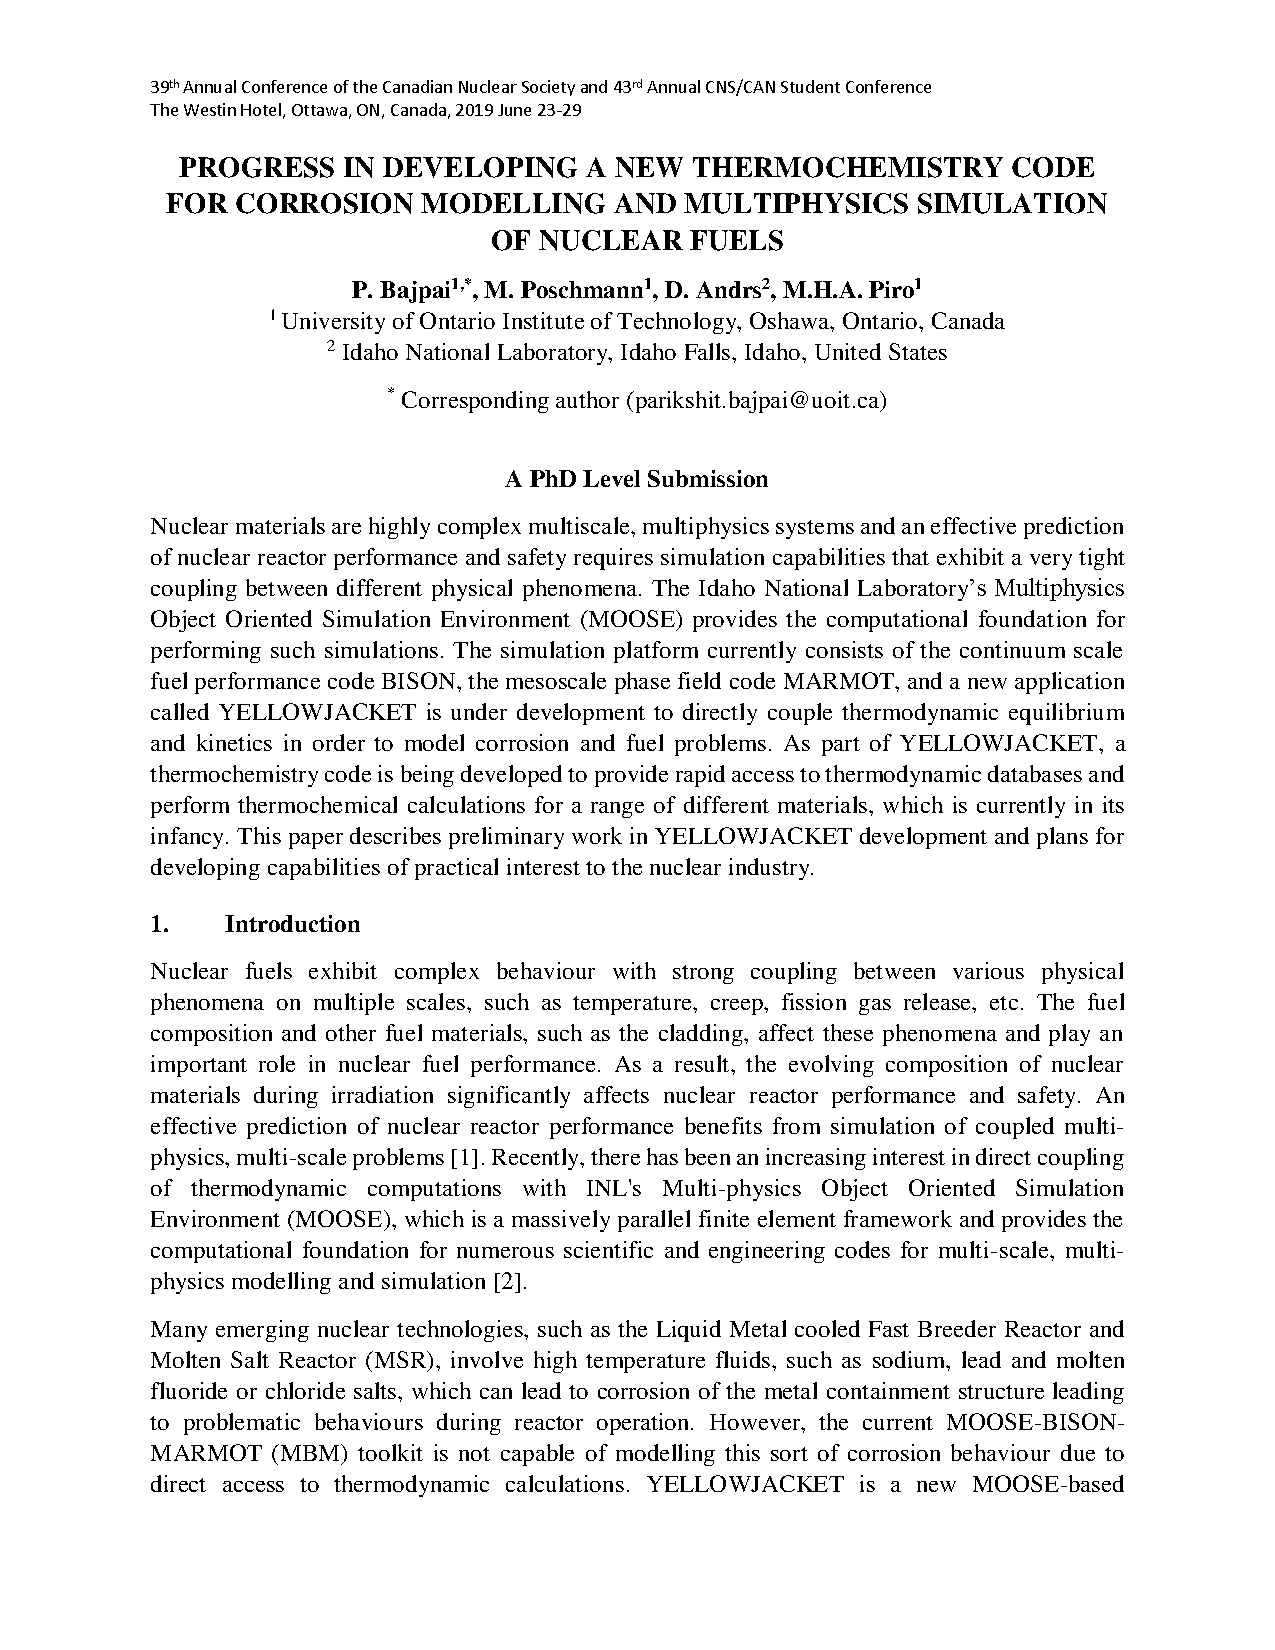
\includepdf[pages=-]{publications/Bajpai_CNS_2019.pdf}

\setboolean{@twoside}{false}


%\newpage
%\cleardoublepage
%\thispagestyle{empty}
%\begin{figure}
%	\centering
%	\includegraphics[width=\textwidth]{figures/YJ_cartoon}
%\end{figure}

\end{document}

